% concatenated from jmlr_revision.tex
\documentclass[twoside,11pt]{article}

\usepackage{blindtext}
% Any additional packages needed should be included after jmlr2e.
% Note that jmlr2e.sty includes epsfig, amssymb, natbib and graphicx,
% and defines many common macros, such as 'proof' and 'example'.
%
% It also sets the bibliographystyle to plainnat; for more information on
% natbib citation styles, see the natbib documentation, a copy of which
% is archived at http://www.jmlr.org/format/natbib.pdf

% Available options for package jmlr2e are:
%
%   - abbrvbib : use abbrvnat for the bibliography style
%   - nohyperref : do not load the hyperref package
%   - preprint : remove JMLR specific information from the template,
%         useful for example for posting to preprint servers.
%
% Example of using the package with custom options:
%
% \usepackage[abbrvbib, preprint]{jmlr2e}

\usepackage[abbrvbib, preprint]{jmlr2e}
% additional packages
\usepackage[english]{babel}
\usepackage[letterpaper,top=2cm,bottom=2cm,left=2.5cm,right=2.5cm,marginparwidth=1.75cm]{geometry}
\usepackage{advdate}
\usepackage{algorithm}
\usepackage{algpseudocode}
\usepackage{amsmath}
\usepackage{amssymb}
\usepackage{booktabs}
\usepackage{braket}
\usepackage{caption}
\usepackage{enumitem}
%\usepackage[numbers]{natbib}
\usepackage{bbm}
% \usepackage{mathrsfs}
\usepackage{mathtools}
\usepackage{soul}
\usepackage{subcaption}
\usepackage{tikz}
\usetikzlibrary{arrows.meta, positioning}

\usepackage{xcolor}
\usepackage{graphicx}
%\usepackage[colorlinks=true, allcolors=blue]{hyperref}
% \newtheorem{theorem}{Theorem}[section]  % Master counter for numbering
% \newtheorem{lemma}[theorem]{Lemma}   
% \newtheorem{prop}[theorem]{Proposition} 
% \newtheorem{ex}[theorem]{Example}    
% \newtheorem{remark}[theorem]{Remark}  
% \newtheorem{definition}[theorem]{Definition}   
% \usepackage{fancyhdr}

% Definitions of handy macros can go here
\newcommand{\yesterday}{{\AdvanceDate[-1]\today}}
\DeclarePairedDelimiter\floor{\lfloor}{\rfloor}
%math command shortcuts
\newcommand{\dXt}{\mathrm{d}X_t}
\newcommand{\dYt}{\mathrm{d}Y_t}
\newcommand{\dt}{\mathrm{d}t}
\newcommand{\dx}{\mathrm{d}x}
\newcommand{\dWt}{\mathrm{d}W_t}

\newcommand{\N}{\mathbb{N}}
\newcommand{\C}{{\mathbb C}}
\newcommand{\R} {\mathbb R}
\newcommand{\Z} {\mathbb Z}
\newcommand{\Q} {\mathbb Q}
\newcommand{\Si} {\mathbb S}
\newcommand{\Hi} {\mathbb H}
\newcommand{\Ti} {\mathbb T}
\newcommand{\F} {\mathcal{F}}
\newcommand{\B} {\mathcal{B}}
\newcommand{\G} {\mathcal{G}}
\newcommand{\E} {\mathbb{E}}
\newcommand{\var} {\mathop{Var}}
\newcommand{\cov} {\mathrm{Cov}}
\newcommand{\I}{\mathbbm{1}}
\newcommand{\Id}{\mathrm{I}_d}
\newcommand{\tod}{\xrightarrow[]{\text{d}}}
\newcommand{\toprob}{\xrightarrow[]{\text{p}}}
\newcommand{\indep}{\perp\!\!\!\!\perp} 
\DeclareMathOperator{\sgn}{sgn}
\DeclareMathOperator*{\argmax}{arg\,max}
\DeclareMathOperator*{\argmin}{arg\,min}
\newcommand{\todo}[1]{\textbf{\textcolor{red}{TODO: #1}}}
\newcommand{\rv}[1]{\textcolor{black}{#1}}
\newcommand{\gs}[1]{\textcolor{red}{[#1]}}
\newcommand{\hr}[1]{\textcolor{brown}{[#1]}}
\newcommand{\vg}[1]{\textcolor{blue}{[#1]}}
\newcommand{\sz}[1]{\textcolor{purple}{[#1]}}

\usepackage[capitalize]{cleveref}

% Heading arguments are {volume}{year}{pages}{date submitted}{date published}{paper id}{author-full-names}

\usepackage{lastpage}
\jmlrheading{23}{2025}{1-\pageref{LastPage}}{1/21; Revised 5/22}{9/22}{21-0000}{Vincent Guan, Joseph Janssen, Hossein Rahmani, Andrew Warren, Stephen Zhang, Elina Robeva and Geoffrey Schiebinger}

% Short headings should be running head and authors last names

\ShortHeadings{Identifying Drift, Diffusion, and Causal Structure from Temporal Snapshots}{Guan, Janssen, Rahmani, Warren, Zhang, Robeva, and Schiebinger}
\firstpageno{1}

\begin{document}

\title{Identifying Drift, Diffusion, and Causal Structure from Temporal Snapshots}

\author{\name Vincent Guan \email vguan23@math.ubc.ca \\
       \addr Department of Mathematics\\
       University of British Columbia, Vancouver, Canada
       \AND
       \name Joseph Janssen \email joejanssen@eoas.ubc.ca \\
       \addr Department of Earth, Ocean and Atmospheric Sciences\\
       University of British Columbia, Vancouver, Canada
       \AND
       \name Hossein Rahmani \email hrahmani@math.ubc.ca \\
       \addr Department of Mathematics\\
       University of British Columbia, Vancouver, Canada
       \AND
       \name Andrew Warren \email awarren@math.ubc.ca \\
       \addr Department of Mathematics\\
       University of British Columbia, Vancouver, Canada
       \AND
       \name Stephen Y. Zhang \email syz@syz.id.au \\
       \addr School of Mathematics and Statistics\\
       University of Melbourne, Melbourne, Australia
       \AND
       \name Elina Robeva \email erobeva@math.ubc.ca \\
       \addr Department of Mathematics\\
       University of British Columbia, Vancouver, Canada
       \AND
       \name Geoffrey Schiebinger \email geoff@math.ubc.ca \\
       \addr Department of Mathematics\\
       University of British Columbia, Vancouver, Canada}

% \author{Vincent Guan$^1$ \and Joseph Janssen$^1$ \and Hossein Rahmani$^1$ \and Andrew Warren$^1$ \and Stephen Zhang$^2$  \and Elina Robeva$^1$ \and Geoffrey Schiebinger$^1$}

% \date{%
%     $^1$University of British Columbia\\%
%     $^2$University of Melbourne\\[2ex]%
%     \yesterday
% }

\editor{My editor}

\maketitle

\begin{abstract}%   <- trailing '%' for backward compatibility of .sty file
Stochastic differential equations (SDEs) are a fundamental tool for modelling dynamic processes, including gene regulatory networks (GRNs), contaminant transport, financial markets, and image generation. However, learning the underlying SDE from data is a challenging task, especially if individual trajectories are not observable. Motivated by burgeoning research in single-cell datasets, we present the first comprehensive approach for jointly identifying the drift and diffusion of an SDE from its temporal marginals. Assuming linear drift and additive diffusion, we \rv{show that non-identifiability can only arise if the initial distribution possesses generalized rotational symmetries. We further prove that even if this condition holds, the drift and diffusion can almost always be recovered from the marginals. Additionally, we show that the causal graph of any SDE with additive diffusion can be recovered from the identified SDE parameters.} To complement this theory, we adapt entropy-regularized optimal transport to handle anisotropic diffusion, and introduce APPEX (Alternating Projection Parameter Estimation from $X_0$), an iterative algorithm designed to estimate the drift, diffusion, and causal graph of an additive noise SDE, solely from temporal marginals. We show that APPEX iteratively decreases Kullback–Leibler divergence to the true solution, and demonstrate its effectiveness on simulated data from linear additive noise SDEs.
\end{abstract}

\begin{keywords}
Stochastic differential equations (SDEs), optimal transport, trajectory inference, causal inference, Schrodinger Bridge
\end{keywords}


\section{Introduction}
% check out Radionuclide migration at experimental polygon at Red Forest waste site in Chernobyl zone. Part 2: Hydrogeological characterization and groundwater transport modeling + GEOLOGY STRUCTURE AND HYDROGEOLOGY CONDITIONS OF THE CHERNOBYL PILOT SITE + Virus and Bacteria Transport in a Sandy Aquifer, Cape Cod, MA + Preliminary observations on bacterial transport in a coastal plain aquifer to motivate real data study
This work presents the first comprehensive approach for jointly identifying the drift and diffusion of a stochastic differential equation (SDE) from observed temporal marginals. While parameter estimation has been studied extensively using trajectory data, either from one long trajectory \citep{nielsen2000parameter, bishwal2007parameter}, or multiple short trajectories \citep{manten2024signature, lu2021learning, pawlowicz2019lagrangian}, it is often impossible to observe individual trajectories when tracking large populations. For example, in single-cell RNA sequencing (scRNA-seq) datasets, the destructive nature of sequencing technologies prevents specific cells from being tracked over time \citep{trapnell2014dynamics, setty2016wishbone, farrell2018single}. Similarly, hydrogeochemical sensors cannot track distinct particles when studying contaminant flow, providing only data on plume migration \citep{man2007stochastic, hazas2023evolution,salamon2007modeling,elfeki2006prediction,adams1992field,boggs1992field,mackay1986natural,nenna2011application}. Observational data may therefore be limited to samples from temporal marginals of the process at various measurement times. We refer to this observational setting as \textit{marginals-only}.

Many stochastic processes are not identifiable under the marginals-only setting, since their distributions may evolve identically, despite having distinct parameter sets \citep{weinreb2018fundamental}. Previous works therefore simplify the problem by assuming that the drift is irrotational and that the diffusion is isotropic, with known diffusivity \citep{weinreb2018fundamental, lavenant2021towards,vargas2021solving,chizat2022trajectory}.

% In this work, we prove in Theorem \ref{thm: identifiability} that non-identifiability under the time-homogeneous linear additive noise SDE model is resolved if the initial distribution $X_0$ is not auto-rotationally invariant (see Definition \ref{def:autorotationalinvariant}). We further introduce a practical method for estimating the drift and diffusion of a general additive noise process, without prior knowledge or additional assumptions, and extensively demonstrate its effectiveness on simulated data.
% are powerful probabilistic models for capturing the dynamics of processes influenced by randomness and uncertainty. Random noise can come from a system's internal fluctuations, such as molecular or cellular interactions. Noise can also be introduced by external factors, whose influence may be unknown or poorly understood. 
% Scientists are particularly interested in learning the data generating processes underlying dynamical systems.
% This is typically done by inferring the deterministic and random parts of the SDE, commonly referred to as drift and diffusion. 
% More generally, this work is relevant to any domain where one wants to learn the data generating process of a system from observed temporal marginals.
% only population-level dynamics are observable rather than individual dynamics.

\subsection{Our contributions}

\rv{We prove that the drift, diffusion, and underlying causal graph of an SDE with linear drift and additive diffusion are generically identifiable (meaning they can be uniquely recovered from the data for almost every SDE parameter configuration) from its temporal marginals.} We also introduce a practical algorithm for estimating each of these quantities solely from the marginals of a general additive diffusion process, and demonstrate the effectiveness of our method on simulated data.
% We consider time-homogeneous linear additive SDEs, which is the most studied model \citep{wang2024generator, yachimura2023scegot, lobus2014absolute, zhang2024joint, rohbeck2024bicycle}. We derive conditions that make this inference possible, and develop a method to perform the joint inference. 
We illustrate our theoretical contributions in Figure \ref{fig:APPEX_main_figure} and our algorithmic contributions in Figure \ref{fig:estimation_steps}. A detailed overview of our contributions is also given below. 

\begin{figure}
\centering
\begin{minipage}{0.45\textwidth}
    \centering
    \begin{subfigure}[b]{\textwidth} % Set to full width of minipage
        \centering
        % Add -5pt offset to counteract caption alignment adjustment
        \vspace{-5pt}
        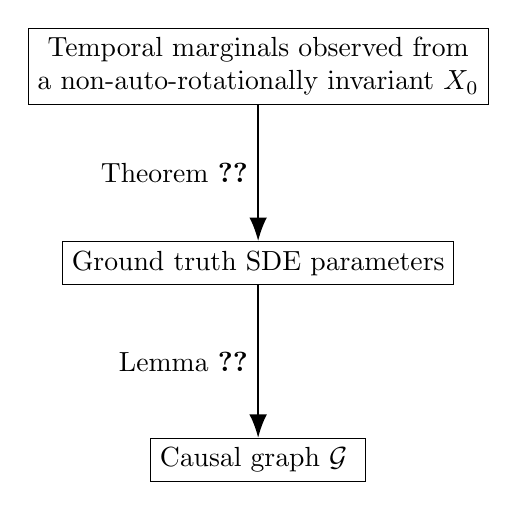
\begin{tikzpicture}[
          rect/.style = {rectangle, draw, minimum width=1cm, minimum height=0.5cm, align=center},
          arrow/.style = {draw, -{Latex[length=3mm]}, thick},
          node distance=1cm
        ]

        % Nodes with fixed coordinates for exact alignment
        \node[rect] (X0) at (0, 0) {Temporal marginals observed from\\ a non-auto-rotationally invariant $X_0$};
        \node[rect] (params) at (0, -2.5) {Ground truth SDE parameters}; 
        \node[rect] (graph) at (0, -5) {Causal graph $\mathcal{G}$ \vphantom{X}}; % Adding \vphantom{} for consistent alignment

        % Arrows
        \draw[arrow] (X0) -- (params) node[midway, left, align=center] {Theorem \ref{thm: identifiability}};
        \draw[arrow] (params) -- (graph) node[midway, left] {Lemma \ref{prop: identify_causal_graph_SDE_add_noise}};

        \end{tikzpicture}
        
        % Adjust caption with 5pt offset to align with the other caption
        \vspace{5pt}
        \caption{Theoretical contributions: identifying drift, diffusion, and causal structure from temporal marginals}
        \label{fig:APPEX_main_figure}
    \end{subfigure}
\end{minipage}%
\hfill
\begin{minipage}{0.45\textwidth}
    \centering
    \begin{subfigure}[b]{\textwidth} % Set to full width of minipage
        \centering
        % Add -45pt offset to counteract caption alignment adjustment
        \vspace{25pt}
        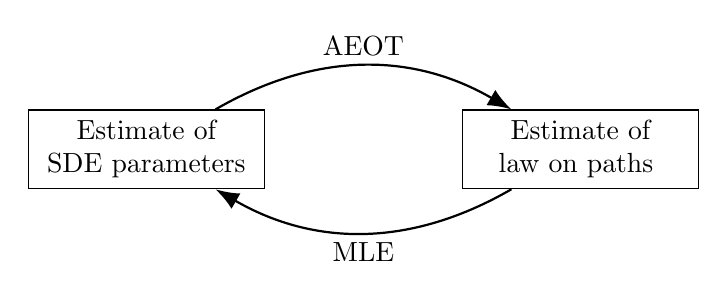
\begin{tikzpicture}[
          rect/.style = {rectangle, draw, minimum width=3cm, minimum height=1cm, align=center},
          arrow/.style = {draw, -{Latex[length=3mm]}, thick},
          node distance=1cm
        ]

        % Nodes with matching coordinates for alignment
        \node[rect] (est_params) at (0, -2.5) {Estimate of\\
        SDE parameters}; % Matched coordinate to "Ground truth SDE parameters"
        \node[rect, right=of est_params, xshift=1.5cm] (est_law) {Estimate of\\ law on paths \vphantom{X}}; % Adding \vphantom{} for consistent alignment

        % Arced edges
        \draw[arrow, bend left=30] (est_params) to node[midway, above] {AEOT} (est_law);
        \draw[arrow, bend left=30] (est_law) to node[midway, below] {MLE} (est_params);

        \end{tikzpicture}
        
        % Adjust caption with 45pt offset to align with the other caption
        \vspace{40pt}
        \caption{Algorithmic contributions: APPEX algorithm}
        \label{fig:estimation_steps}
    \end{subfigure}
\end{minipage}

\caption{Outline of our theoretical (a) and algorithmic (b) contributions. In (b), our algorithm Alternating Projection Parameter Estimation from $X_0$ alternates between Anisotropic Entropy-regularized Optimal Transport (AEOT) and Maximum Likelihood Estimation (MLE).}
\label{fig:contributions_figure}
\end{figure}


\begin{enumerate}
    \item We provide a theoretical foundation for system identification from temporal marginals.\begin{enumerate}
        \item  \rv{In Section \ref{sec:identify}, we prove identifiability conditions for jointly recovering the drift and diffusion of a linear additive noise SDE from continuously observed marginals. In \cref{thm: identifiability}, we prove that unidentifiable parameter configurations exist if and only if the initial distribution possesses generalized rotational symmetries, a condition we call auto-rotational invariance (ARI). Then, \cref{thm:stronger} provides a stronger unconditional guarantee: even when the initial distribution is ARI, the set of unidentifiable configurations has measure zero. Thus, linear additive noise SDEs are generically identifiable.}
        % \rv{In Section \ref{sec:identify}, we prove identifiability conditions for jointly recovering the drift and diffusion of a linear additive noise SDE from continuously observed marginals. In \cref{thm: identifiability}, we prove that non-identifiability in this setting is feasible if and only if that the initial distribution possesses generalized rotational symmetries, a condition that we call auto-rotational invariance (ARI). Then, in \cref{thm:stronger}, we prove that generic identifiability holds even if the initial distribution obeys ARI. Together, our results show that non-identifiability requires both a pathological initial distribution and a pathological SDE parameter configuration from a measure $0$ set in the parameter space.}
        
        % \todo{Revise} In Theorem \ref{thm: identifiability}, we fully characterize the conditions for guaranteeing identifiability of linear drift and additive diffusion from observed marginals. Identifiability is guaranteed if and only if the initial distribution $X_0$ is not auto-rotationally invariant (Definition \ref{def:weak_ari}). 
        \item In Section \ref{sec:causal_graph}, 
        % Lemma \ref{prop: identify_causal_graph_SDE_add_noise}, 
        we connect parameter estimation to causal structure learning via dynamic structural causal models \citep{boeken2024dynamic}. We show that the causal graph of any additive noise model can be recovered from the identified SDE parameters.
    \end{enumerate}
    \item In Section \ref{sec:methods}, we introduce our algorithm: Alternating Projection Parameter Estimation from $X_0$ (APPEX). \rv{It is the first Schr\"odinger Bridge based method designed to estimate drift and diffusion from temporal marginals of additive noise SDEs, without prior knowledge.}
    \begin{enumerate}
        \item We show that with each iteration, APPEX's estimates approach the true solution. APPEX alternates between a trajectory inference step, which is a Schr\"odinger bridge problem, and a parameter estimation step, which is solved via maximum likelihood estimation. 
        % We show that both subprocedures are optimal with respect to the Kullback-Leibeler (KL) divergence.
        \item To solve the Schr\"odinger bridge problem for trajectory inference, we adapt entropic optimal transport for parameter dependent transport costs, including arbitrary anisotropic diffusion.
        \item We test APPEX's efficacy across a wide range of experiments in Section \ref{sec:experiments}. We first use APPEX to empirically demonstrate that classical non-identifiable linear additive noise SDEs are resolved when $X_0$ is initialized appropriately according to Theorem \ref{thm: identifiability}.
        We then demonstrate APPEX's effectiveness over a large-scale experiment on higher dimensional SDEs with randomly generated parameter sets. Our results demonstrate that APPEX identifies arbitrary linear additive noise SDEs with significantly higher accuracy than the widely-used Waddington-OT (WOT) method \citep{schiebinger2019optimal}. Our final experiments demonstrate that APPEX can be used to identify the system's causal graph, even in the presence of correlated diffusion from latent confounders.
    \end{enumerate}
\end{enumerate}

\section{Background and related work}
In this section, we first give an overview of SDEs and a discussion of some real-world applications. We then review relevant literature and techniques for statistical inference from the ``marginals-only" observational setting. Finally, we discuss the problem of non-identifiability of SDEs under this setting.
% SDEs have also seen prominent usage for applications in computer vision \citep{cao2023exploring,croitoru2023diffusion}, and option pricing \citep{black1973pricing}. 
% SDEs have long been used to model natural processes \citep{oh2010stochastic,delay2005simulating,lande2003stochastic,schiebinger2019optimal}, where the drift and diffusion have meaningful physical interpretations.

\subsection{Stochastic differential equations (SDEs) and modeling real-world systems}
The mathematical framework of SDEs, or drift-diffusion processes, originates from statistical mechanics. In such applications, the drift models the velocity of particles flowing in a carrier fluid, while diffusion is driven by Brownian motion, and governs their dispersion due to random collisions \citep{einstein1956investigations, macinnes1992stochastic}. Formally, a $d$-dimensional time-homogeneous SDE is driven by an $m$-dimensional Brownian motion $W_t$, and is parameterized by a drift function $b(x): \R^d \to \R^d$ and a diffusion function $\sigma(x): \R^d \to \R^{d \times m}$, such that
\begin{equation}
    \mathrm{d}X_t = b(X_t) \:\mathrm{d}t+ \sigma(X_t)\: \mathrm{d}W_t, \  X_0 \sim p_0,
    \label{eq: general_SDE}
\end{equation}
where $b(x)$ and $\sigma(x)$ are Lipschitz to ensure the solution's existence and uniqueness \citep{fang2020adaptive}.

By capturing deterministic and stochastic dynamics, SDEs provide a powerful framework for modeling complex systems across a variety of fields. For example, SDEs have been used to model cell differentiation in single-cell biology, where a stem cell changes into another cell type, such as a blood cell or bone cell. 
% This process is often visualized with Waddington's epigenetic landscape, where cells figuratively traverse a developmental terrain, guided by deterministic forces (drift) and stochastic fluctuations (diffusion) \citep{waddington1935animal,waddington1957strategy,schiebinger2019optimal}.
The drift can be related to the set of genes that directly regulate the expression of a gene of interest \citep{zhang2024joint,aalto2020gene,atanackovic2024dyngfn,zhao2024optimal,tejada2023causal}, and therefore provides insights into genetic diseases and gene therapies. Meanwhile, the diffusion informs the extent to which cell fates are determined by initial conditions \citep{forrow2024consistent}. In hydrological systems, drift is linked to important and unknown properties of the subsurface, such as hydraulic conductivity through average flow velocity \citep{hazas2023evolution,beven1993dispersion}, while the diffusion usually describes material heterogeneity or turbulence \citep{beven1993dispersion}, and therefore informs the applicability of popular models, such as Darcy's law \citep{man2007stochastic,oh2010stochastic,lichtner2002new}. Together, these parameters determine pollutant fates in hydrological systems, a key concern in safeguarding drinking water sources \citep{o2002part,frind2006well,locatelli2019simple,chen1999assessment,paulson1997transport,cahill2019advancing}. In addition to applications to physical sciences, SDEs have also been prominently used for pricing stocks and options in financial markets \citep{black1973pricing} and for image generation in computer vision \citep{meng2021sdedit}. 

\subsection{Linear additive noise SDEs}
In this paper, we focus on time-homogeneous additive noise SDEs. These SDEs are characterized by an arbitrary drift function $b(X_t)$ and a possibly anisotropic space-independent diffusion $G \in \mathbb{R}^{d \times m}$, such that 
\begin{equation}
    \mathrm{d}X_t = b(X_t) \:\mathrm{d}t+ G\: \mathrm{d}W_t, \  X_0 \sim p_0.
    \label{eq: additive_noise_SDE}
\end{equation}
We also refer to $H = GG^\top \in \R^{d \times d}$ as the (observational) diffusion, since it is only possible to \rv{identify} $H$ \citep{wang2024generator, pavliotis2014stochastic}. Time-homogeneous linear additive noise SDEs are of particular interest \citep{du2023dynamical, wang2024generator, zhang2024joint}, as they generalize the popular Ornstein-Uhlenbeck process. A time-homogeneous linear additive noise SDE obeys the form:
\begin{equation}
    \mathrm{d}X_t = AX_t \: \mathrm{d}t+ G\:\mathrm{d}W_t, \ \ X_0 \sim p_0, \ \ A \in \R^{d \times d}.
    \label{eq: linear_additive_noise_SDE}
\end{equation}
We overview important properties of this SDE in Section \ref{sec:linear_additive_noise} of the appendix, including its closed form solution and transition density.




% These processes have since seen prevalent usage across a broad range of applications, including stock and options pricing \citep{black1973pricing}, and image generation \citep{meng2021sdedit}.
% , such as contaminant transport \citep{oh2010stochastic,delay2005simulating}, population dynamics \citep{lande2003stochastic}, and gene expression trajectories \citep{schiebinger2019optimal}.

% Estimating diffusion is also important because the diffusion influences the fate of cells moving to various steady-states or wells \citep{forrow2024consistent}. While small diffusion implies that cell fates are mostly determined by their initial conditions, large-scale diffusion implies that cell fates are significantly influenced by random or unknown processes \citep{forrow2024consistent}. 



% In some models, drift and diffusion are also directly dependent on one another, as in the chemical Langevin equation \citep{gillespie2000chemical,chardes2023stochastic} and the advection-dispersion equation for solute transport \citep{hazas2023evolution,lichtner2002new,beven1993dispersion}. We remark that even when the drift and diffusion are independent, these parameters remain inextricably linked, as they jointly explain the dynamics of the underlying process. \\

% Indeed, we will show that a robust estimate of one parameter is typically only achievable given a reliable estimate of the other. \\

% often 
% primarily studied for applications, including genetic trajectory inference \citep{schiebinger2019optimal, weinreb2018fundamental, lavenant2021towards, chizat2022trajectory, yachimura2023scegot, shen2024multi, zhang2024joint} and gene regulatory network (GRN) inference \citep{aalto2020gene, zhao2024optimal, atanackovic2024dyngfn, rohbeck2024bicycle, zhang2024joint} provide insights into genetic diseases and gene therapies. 


% As we will show, a robust estimate of one parameter is typically only achievable given a reliable estimate of the other. 




% Regardless of the observational setting, drift and diffusion fundamentally determine the system's causal structure and trajectory fates, making parameter estimation a principal objective across various areas of research.
% One of the principal goals of stochastic analysis is to learn the drift and diffusion parameters of a process' underlying SDE, in order to understand the system's dynamics.
% \noindent
% \textbf{Inference from temporal marginals.}
\subsection{Inference from temporal marginals}
The marginals-only observational setting dates back to at least Aristotle, who dissected bird eggs at various developmental stages, in order to infer the processes and mediators (e.g., heat) behind embryogenesis \citep{waddington1935animal,ogle1882aristotle,aristotle1942generation}. If the underlying system is modeled by an SDE, then the evolution of its temporal marginals $p_t$ are defined by its Fokker-Planck equation. For example, a straightforward computation shows that the marginals of a linear additive noise SDE evolve according to the following Fokker-Planck equation:
\begin{equation}
    \frac{\partial}{\partial t}p(x,t) = -\nabla \cdot \left((Ax) p(x,t)\right) + \frac{1}{2} \nabla \cdot (H \nabla p(x,t)), \ \ p(x,0)=p_0(x).
    \label{eq: FP_linear_additive_noise}
\end{equation}
 % Although \eqref{eq: FP_linear_additive_noise} assumes differentiability, we note that the Fokker-Planck equation can also be defined in the weak distributional sense for general probability measures $p_t$ (see Appendix Section \ref{sec: weak_FP}). 

Contemporary research in statistical inference from temporal marginals largely comes from single-cell biology. Many works focus on trajectory inference for cell fates \citep{schiebinger2019optimal, lavenant2021towards,yachimura2023scegot, chizat2022trajectory}, while others infer the causal graph (GRN) \citep{aalto2020gene,brouillard2020differentiable, tejada2023causal, rohbeck2024bicycle}, or perform parameter estimation \citep{chakraborty2009parameter, shen2024learning}. Recent works jointly estimate a subset of these quantities by leveraging their intrinsic relationships. For instance, \citet{vargas2021solving} and \citet{shen2024multi} are primarily interested in trajectory inference, and iteratively estimate drift and trajectories. Meanwhile, \citet{zhang2024joint} iteratively estimates drift and trajectories, while additionally applying permanent interventions on the drift dynamics for network inference. 

% Our approach does not assume irrotational drift or isotropic diffusion, and does not require additional interventions. 
% Ultimately, drift and diffusion are central to the system's causal structure and trajectory fates





% SDEs crucially depend on both deterministic and random relationships, and it is difficult to precisely know these relationships beforehand.


% Furthermore, a large number of these permanent interventions are required in order to learn the linear dynamical system. In simulations, $10\%$ of all observed genes are eliminated from the dynamical system, amounting to $2000$ gene knockouts. In contrast, we show that we can identify any linear additive noise SDE by intervening solely on the initial distribution $p_0$
\subsection{Schr\"odinger bridge problem}
Given a set of temporal marginals, trajectory inference is the task of estimating a law on paths that obeys each marginal constraint while closely approximating desired reference dynamics. This is commonly implemented by solving the Schr\"odinger Bridge (SB) problem \citep{chizat2022trajectory, shen2024learning}, defined below for a pair of marginals. Given the transition law $\mathcal{K}$ of a reference process, an initial distribution $\mu$, and a final distribution $\nu$, the SB solution is the law of the stochastic process, which satisfies both marginal constraints, while minimizing relative entropy to $\mathcal{K}$:
\begin{equation}
\pi^* = \text{Proj}_{\Pi(\mu,\nu)}^{KL}(\mathcal{K}) = \argmin_{\pi \in \Pi(\mu,\nu)} D_{KL}(\pi \| \mathcal{K}).
\label{eq: schrodinger_bridge}
\end{equation}


The SB problem has also gained interest in the machine learning community, due to its connection to generative diffusion models. Score estimation of time-reversed SDEs is an instance of the SB problem \citep{de2021diffusion}, and SB solvers are now widely used in generative modeling due to their flexibility \citep{de2021diffusion, chen2021likelihood, shi2024diffusion, huang2024one}. 
% Furthermore, the solution to the SB problem can itself be represented as a function of forwards and backwards drifts \citep{vargas2021solving}. 

\subsection{Identifiability of SDE parameters}
The problem of non-identifiability occurs if there exists an alternative drift-diffusion pair, e.g. $(\tilde{A}, \tilde{H}) \neq (A, H)$ for linear-additive noise SDEs, which shares the same marginals. Equivalently, the processes satisfy the same Fokker-Planck equation across all observed times, given initial distribution $p_0$. Non-identifiability can occur due to many factors. For example, distinct SDEs can share the same stationary distribution, and would hence be non-identifiable from marginals if $p_0$ is initialized at equilibrium \citep{lavenant2021towards, shen2024learning}. Also, if the initial distribution is standard normal $p_0 \sim \mathcal{N}(0, I_d)$, then it would be impossible to distinguish between a pure Brownian motion, and an SDE with an additional rotational vector field \citep{shen2024learning}. We  overview three classical examples of non-identifiability in Section \ref{sec:Noniden_examples} of the Appendix.

Because of non-identifiability, previous works require assumptions about the underlying SDE to perform inference. The standard assumptions are that the drift is an irrotational vector field $\nabla \psi$ \citep{weinreb2018fundamental, lavenant2021towards, vargas2021solving, chizat2022trajectory, terpin2024learning} and that the diffusion is both known and given by isotropic Brownian motion $\sigma \mathrm{d}W_t$ \citep{weinreb2018fundamental, lavenant2021towards, vargas2021solving, chizat2022trajectory, shen2024multi, zhang2024joint, terpin2024learning}. It is also common to leverage additional perturbational data from interventions, and to impose regularization, to better learn the system  \citep{rohbeck2024bicycle, zhang2024joint,maddu2024inferring}. However, these constraints impose unrealistic conditions on the data. An irrotational drift field cannot model negative feedback loops or repressilator dynamics, which are common in biological data \citep{weinreb2018fundamental}. Similarly, isotropic diffusion cannot model variable noise scales or correlated noise structures, which commonly arise in real data \citep{mogensen2022graphical, rohbeck2024bicycle, santos2024learning}. While most works use a known diffusion estimate to infer drift, \citet{forrow2024consistent} infers diffusion, but requires a drift estimate. In both cases, the accuracy of the prior estimate is crucial, because misspecified diffusion typically leads to poor drift estimation and vice-versa \citep{beven1993dispersion,guan2025gradient}. This is problematic, since knowing an accurate estimate of drift or diffusion {\em a priori} is unrealistic in practice. Finally, we note that recent work estimates drift and diffusion, but does not consider the uniqueness of learned parameters, due to non-identifiability \citep{terpin2024learning, brogat2024learning}.

To advance the field of statistical inference from temporal marginals, we work to remove previous assumptions by determining conditions for identifiability and designing a method that leverages them. \citet{wang2024generator} showed that identifiability of a linear additive noise SDE from ground truth trajectories with fixed $X_0 \in \R^d$ is equivalent to a non-degenerate rank condition based jointly on $X_0$, the linear drift $A$ and the observational diffusion $GG^\top$. In contrast, our work studies identifiability of linear additive noise SDEs in the more general ``marginals-only" setting. We also demonstrate that identifiability from continuous observation can be guaranteed across all linear additive noise SDEs solely by checking the initial distribution. To the best of our knowledge, this has not been shown even in the case of trajectory-based observations.

\section{\rv{Identification of linear SDEs from temporal marginals}}
\label{sec:identify}

\rv{In this section, we prove three identifiability results of increasing generality, which provide conditions for uniquely recovering the drift and diffusion of linear additive noise SDEs. Our theory demonstrates that SDE non-identifiability is only possible when the observed marginals share a generalized rotational symmetry. Furthermore, identifiability holds under generic conditions, since the set of SDE parameters that can preserve these symmetries over the course of the continuous evolution has Lebesgue measure $0$.}

\rv{\subsection{SDE identifiability under isotropic diffusion}
\label{sec: SDE_param_identifiability_isotropic}
We first consider the case of SDEs with linear drift and isotropic diffusion:
\begin{align}
    dX_t = AX_t \dt + \sigma \dWt,
    \label{eq: isotropic_linear_sde}
\end{align}
and we consider the question of when we can jointly identify the drift $A$ and diffusivity $\sigma^2$ from continuously observed marginals $(p_t: t \ge 0)$. It turns out that non-identifiability is intrinsically related to the marginals sharing a generalized rotational symmetry. We now define what we mean by a generalized rotation.
\begin{definition}[Generalized rotation]
\label{def:generalized_rotation}
Let $d \ge 2$. We define a $\Sigma$-generalized rotation in $\R^d$ as a matrix exponential $e^{B\theta}$, such that $\theta$ is the rotation angle and $B \in \R^{d \times d}$ is skew-symmetric with respect to $\Sigma \succeq 0$, i.e. $B\Sigma + \Sigma B^\top = 0$. 
\end{definition}
Note that classical rotations only differ in that the matrix $B$ must be skew-symmetric, which corresponds to restricting $\Sigma = I_d$. By allowing $\Sigma \neq I_d$, we enable rotations to be defined over anisotropic geometries. If $\Sigma \succeq 0$ is full rank, then $\Sigma$-generalized rotations are equivalent to classical rotations in a transformed space, such that lengths and angles are modified by scaling and shearing (see Lemma \ref{lem:conjugate_rotation} in appendix). We also note that if $\Sigma \succeq 0$ is rank-deficient, then $B$ can take any values in the nullspace of $\Sigma$. We now extend this notion to random variables, by defining a distribution $X$ to be \emph{auto-rotationally invariant} (ARI) if its law (distribution) is invariant to the action $e^{B\theta}$ for some nonzero matrix $B \in \R^{d \times d}$.
\begin{definition}[Auto-rotational invariance]
\label{def:full_ARI}
Let $d \ge 2$. We define a $d$-dimensional random variable $X$ to be auto-rotationally invariant (ARI) if there exists some square matrix $B \neq 0$, such that for all $\theta \in \R$, $e^{B\theta}X \sim X$. For the case $d=1$, we by convention consider mean-zero  Gaussians $\mathcal{N}(0,\sigma^2)$ as the only ARI distributions.
\end{definition}
We term this property auto-rotational invariance to reflect its two constituent features. First, the transformation $e^{B\theta}$ constitutes a generalized rotation (Definition \ref{def:generalized_rotation}) with respect to the distribution’s own covariance $\Sigma = \text{cov}(X)$ (see Lemma \ref{lem: lyapunov_condition}), hence \textit{auto-rotational}. Second, the distribution is invariant under this action ($X \sim e^{B\theta}X$). Auto-rotational invariance is a highly restrictive property since it requires that the law of the random variable is rotationally symmetric with respect to the geometry imposed by its covariance $\Sigma$. If $\Sigma \succeq 0$ is full rank, then $X$ being ARI implies that it has a density with elliptic level sets (see Lemma \ref{lemma:level_sets}). However, we note that all rank degenerate distributions are auto-rotationally invariant (see Lemma \ref{lemma: degenerate_X_isotropy}), since $e^{B\theta}$ can be designed to operate outside the distribution's support.} 

\rv{We now show present our first identifiability result, which states that the SDE parameters $(A, \sigma^2)$ can be uniquely identified from continuously observed marginals $X_t \sim p_t$, unless each marginal is auto-rotationally invariant with respect to the same generalized rotation $e^{B\theta}$.
\begin{theorem}[Identifiability under isotropic diffusion]
Suppose that the observed marginals $(p_t: t \ge 0)$ can be produced by multiple distinct parameter sets $(A,\sigma^2) \neq (\tilde{A},\tilde{\sigma}^2)$. Then, each marginal $X_t \sim p_t$ is auto-rotationally invariant with respect to the same generalized rotational action $e^{B\theta}$, i.e. for all marginals $X_t \sim p_t$, we have that $e^{B\theta}X_t \sim X_t$ for all $\theta \in \R$.
\end{theorem}}

\begin{proof}
\rv{First, suppose that distinct parameter sets $(A,\sigma^2) \neq (\tilde{A},\tilde{\sigma}^2)$ produce the same marginals $(p_t: t \ge 0)_{A,\sigma^2} =  (p_t: t \ge 0)_{\tilde{A},\tilde{\sigma}^2}$. Then, their Fokker-Planck evolution equations are equal:
\begin{align*}
    \partial_t p_t(x) &= -\nabla \cdot (Ax p_t(x)) + \frac{\sigma^2}{2}\Delta p_t(x) \\
    &= -\nabla \cdot (\tilde{A}x p_t(x)) + \frac{\tilde{\sigma}^2}{2}\Delta p_t(x).
\end{align*}
Without loss of generality, we may define the residual diffusivity $\bar{\sigma}^2 = \sigma^2-\tilde{\sigma}^2 \ge 0$ and the residual drift $\bar{A} = A- \tilde{A}$. By subtracting the equations, we obtain a stationary Fokker-Planck equation with the residual parameters
\begin{align}
    0&= -\nabla \cdot (\bar{A}x p_t(x)) + \frac{\bar{\sigma}^2}{2}\Delta p_t(x).
    \label{eq:residual_FP}
\end{align}
First, we note that if the residual diffusion $\bar{\sigma}^2 = \sigma^2-\tilde{\sigma}^2$ is nonzero, it follows from elliptic PDE theory that the residual Fokker-Planck equation \eqref{eq:residual_FP} has at most one stationary distribution \citep[Theorem 4.1.6, Example 4.1.8]{bogachev2022fokker}. Since each marginal $p_t$ solves \eqref{eq:residual_FP}, each marginal is in fact the stationary distribution $p_{eq}$. For linear SDEs, $p_{eq}$ is the Gaussian distribution $\mathcal{N}(0, \Sigma)$ with $\Sigma$ satisfying $\Sigma A + A \Sigma = \sigma^2$ \citep[Theorem 6.2.1]{da1996ergodicity}. Thus, if the diffusivities are unequal, then non-identifiability implies that all marginals are observed at a stationary Gaussian distribution, which is auto-rotationally invariant.}

\rv{From this analysis, we may also deduce that if the marginals $(p_t)_{t \ge 0}$ are not all the same distribution, then non-identifiability is only possible if both SDEs share the same diffusivity $\sigma^2$, and are thus only distinct in their drifts. In this case, the residual Fokker-Planck equation reduces to the continuity equation:
\begin{align}
    0&= -\nabla \cdot (\bar{A}x p_t(x)).
\end{align}
By Liouville's theorem (see \citep[Theorem 1]{neklyudov2021deterministic}), each observed marginal $X_t \sim p_t$ is stationary under the linear ODE $\dot{x}=\bar{A}x$. Thus, for each marginal $X_t$, we have
\begin{align}
    e^{\bar{A}\theta}X_t \sim X_t \quad \forall \theta \in \R.
\end{align}
We conclude that each marginal $X_t \sim p_t$ is auto-rotationally invariant with respect to the same matrix $B=\bar{A}$.}
\end{proof}

\rv{We make a couple remarks about this result. First, we recall that observing marginals at equilibrium is a well-documented source of non-identifiability, since equilibrium only depends on the drift to diffusion ratio (see \citet{lavenant2021towards} and \citet[Proposition 4.1]{guan2025gradient}). Our result shows that under isotropic diffusion, observing marginals that vary in time is enough to determine the true diffusivity $\sigma^2$. This follows from the same elliptic PDE argument underlying a recent identifiability result by \citet{guan2025gradient}, which showed that observation at equilibrium is the only source of non-identifiability of the SDE parameters for gradient-flow SDEs, which are defined by conservative drift $-\nabla \Psi$ and isotropic diffusivity $\sigma^2$.}

\rv{However, in contrast to the gradient-flow setting, linear SDEs may have rotational drift, which introduces undetectable rotation as a second source of non-identifiability. Indeed, a classic non-identifiability example from the literature is given by the systems \citep{hashimoto2016learning, shen2024learning}:
\begin{align}
    \mathrm{d}X_t &= \mathrm{d}W_t, &X_0 \sim \delta_0\\
    \mathrm{d}Y_t &= \begin{bmatrix} 0 & 1 \\ -1 & 0  \end{bmatrix}Y_t \: \mathrm{d}t
    + \mathrm{d}W_t, &  Y_0 \sim \delta_0,
\end{align}
where the residual drift is the skew-symmetric matrix $\bar{A}=\begin{bmatrix}
    0 & 1 \\
    -1 & 0
\end{bmatrix}$,
which produces a rotational action that is indistinguishable at the level of the marginals $p_t \sim \mathcal{N}(0, t I_d)$. We present examples with more general rotational geometries in \cref{sec:Noniden_examples}. Our result shows that 
this failure mode, characterized by shared invariance under a generalized rotational action, is the only other source of non-identifiability besides observation at equilibrium, for linear SDEs with isotropic diffusion.}
% Thus, as long as we observe transient marginals, which are not all invariant to a generalized rotational action, $e^{B\theta}$, then we can jointly identify the SDE parameters $(A, \sigma^2)$.

\rv{\subsection{SDE identifiability under anisotropic diffusion}}
\label{sec: SDE_param_identifiability_anisotropic}

\rv{We now consider the more general case of linear additive noise SDEs with possibly anisotropic diffusion:
\begin{align}
    dX_t = AX_t \dt + G \dWt,
    \label{eq: anisotropic_linear_sde}
\end{align}
and we derive identifiability conditions for determining the SDE parameters $(A, H = GG^\top)$ from observed marginals $(p_t: t \ge 0)$. We note that anisotropic diffusion significantly complicates identifiability analysis, since the diffusion level can vary in each dimension. Indeed, anisotropic diffusion can produce non-identifiability such that the distributions are stationary in a subset of components, while otherwise exhibiting transience. Since equilibrium distributions for linear additive noise are mean-zero Gaussians \citep[Sections 4.2 and 4.4]{pavliotis2014stochastic}, we can illustrate this by considering a `Gaussian pancake' initial distribution $X_0 \sim p_0$, where
$X_0^{(1)} \sim \mathcal{N}(0, 1)$ and the remaining components
$X_0^{(2:d)}$ are initialized independently. To produce non-identifiability, we consider two different univariate dynamics that preserve $X_t^{(1)} \sim \mathcal{N}(0, 1)$ and we decouple these first component dynamics from the rest of the system:
\begin{align}
\mathrm{d} X_t &= \begin{bmatrix} -\frac{1}{2} & \mathbf{0} \\ \mathbf{0} & A_{\setminus1} \end{bmatrix} X_t \,\mathrm{d}t + \begin{bmatrix} 1 & \mathbf{0} \\ \mathbf{0} & G_{\setminus1}  \end{bmatrix} \mathrm{d}W_t, \quad X_0 \sim p_0 \\
\mathrm{d}Y_t &= \begin{bmatrix} -2 & \mathbf{0} \\ \mathbf{0} & A_{\setminus1} \end{bmatrix} Y_t \,\mathrm{d}t + \begin{bmatrix} 2 & \mathbf{0} \\ \mathbf{0} & G_{\setminus1}  \end{bmatrix} \mathrm{d}W_t, \quad Y_0 \sim p_0.
\end{align}
These SDEs are non-identifiable from marginals since they are both stationary in the first component, while being trivially identical in other components since they share the same independent complementary dynamics $(A_{\setminus1}, G_{\setminus1})$.}

\rv{From this construction, it is clear that the temporal marginals can be non-identifiable while encapsulating diverse geometries. Thus, in the more general case of anisotropic diffusion, non-identifiability is feasible even if a marginal $X_t \sim p_t$ fails to be auto-rotationally invariant, as defined in Definition \ref{def:full_ARI}. However, by recalling the classical fact that Gaussians are the only random variables that have finitely many nonzero cumulants \citep{marcinkiewicz1939propriete}, and moreover, that the only nonzero cumulant of a mean-zero Gaussian is its covariance, we may consider a natural relaxation of auto-rotational invariance. Instead of defining the invariance relation over the full law, we can define it on all cumulant orders, except $n=2$.}


\rv{\begin{definition}[Weak auto-rotational invariance]
\label{def:weak_ari}
Let $X$ be a $d$-dimensional r.v, and denote by $T_n^X(v, \ldots, v)$ the order $n$ tensor defining the $n$th cumulant of $X$, projected in the direction of $v \in \R^d$, i.e. the $n$th cumulant of the univariate r.v. $v^\top X$. Then, $X$ is weakly auto-rotationally invariant if there exists some nonzero matrix $B \in \R^d \times d$, such that the mean and higher order cumulants $n \ge 3$ obey the invariance:
\begin{align}
    T_n^X(e^{B\theta}v, \ldots,e^{B\theta}v) = T_n^X(v, \ldots, v) \quad \forall n \in \N \setminus \{2\}, \forall  v \in \R^d, \forall \theta \in \R.
    \label{eq:new_ARI}
\end{align}
\end{definition}}

\rv{Under sufficient regularity conditions, such that the cumulants determine the law (e.g. if the cumulant generating function exists), weak auto-rotational invariance becomes full auto-rotational invariance (Definition \ref{def:full_ARI}) precisely when the invariance relation \eqref{eq:new_ARI} also holds for the covariance ($n=2$). We previously noted that if $X$ has rank degenerate covariance, such that it is supported in a proper subspace of $\R^d$, then $X$ would satisfy full ARI for any transformation $e^{B\theta}$, where $B$ acts outside the support of $X$. The same idea extends for random variables that are non-Gaussian in a proper subspace of $\R^d$ when considering weak ARI. Thus, weak ARI also includes distributions with full rank covariance, but which are Gaussian when projected along select directions. Furthermore, similarly to full ARI, if $X$ is nondegenerate and non-Gaussian in all components, then the matrix $B$ must be similar to a skew-symmetric matrix, such that the transformation $e^{B\theta}$ is a rotational action (see Lemma \ref{lemma:ARI_implies_generalized_rotation}). In Figure \ref{fig:ARI_distributions}, we visualize three ARI distributions as well as a Gaussian pancake distribution, which is only weakly ARI.}

\begin{figure}[h!]
\centering
\begin{minipage}{0.4\textwidth}
        \centering
        \begin{subfigure}[b]{\textwidth}
            \centering
            \includegraphics[width=\textwidth]{Figures/sphere_rv.pdf}
            \caption{$X_0$ is spherical and invariant under all classical rotations.}
            \label{fig:sphere_vector_field}
        \end{subfigure}
    \end{minipage}%
    \hfill
    \begin{minipage}{0.4\textwidth}
        \centering
        \begin{subfigure}[b]{\textwidth}
            \centering
            \includegraphics[width=\textwidth]{Figures/cylinder_rv.pdf}
            \caption{$X_0$ is cylindrical (up to shearing and scaling), and is invariant under rotation in the $xy$ plane after transformation.}
            \label{fig:cylinder_vector_field}
        \end{subfigure}
    \end{minipage}
    
    % Second row: Dgenerate and Gaussian Pancake
    \begin{minipage}{0.4\textwidth}
        \centering
        \begin{subfigure}[b]{\textwidth}
            \centering
            \includegraphics[width=\textwidth]{Figures/degenerate_rv.pdf}
            \caption{$X_0$ is degenerate and its support lies in the nullspace of $B=\begin{bmatrix}
                1 & -1 \\ 
                0 & 0
            \end{bmatrix}$ }
            \label{fig:degenerate_rv}
        \end{subfigure}
    \end{minipage}
    \hfill
    \begin{minipage}{0.4\textwidth}
        \centering
        \begin{subfigure}[b]{\textwidth}
            \centering
            \includegraphics[width=\textwidth]{Figures/gaussian_pancake_rv.pdf}
            \caption{$X_0$ is a Gaussian pancake, which is mean $0$ univariate Gaussian in $x$.}
            \label{fig:gaussian_pancake_rv}
        \end{subfigure}
    \end{minipage}%
\caption{We visualize four distributions that satisfy auto-rotational invariance. The first three distributions obey strong auto-rotational invariance (Definition \ref{def:full_ARI}), while the Gaussian pancake is weakly auto-rotationally invariant (Definition \ref{def:weak_ari}).}
\label{fig:ARI_distributions}
\end{figure}

\rv{We now present our second identifiability theorem, which proves that non-identifiability from the marginals of a linear additive noise SDE is only possible if the initial marginal $X_0 \sim p_0$ is weakly auto-rotationally invariant, and furthermore, that there exist non-identifiable systems for any weakly ARI initial distribution $X_0$. Intuitively, non-identifiability is only feasible if there is a symmetry to exploit, and if the initial distribution has such a symmetry, then it is susceptible to non-identifiability.}

\rv{\begin{theorem}[Identifiability for linear additive noise SDEs]
Let $p_0$ be a probability distribution on $\R^d$ with a well-defined moment generating function, and let $$\Theta = \{(A,H): A \in \R^{d \times d}, G \in \R^{d \times m}, H = GG^\top \}$$ denote the set of drift-diffusion pairs under a linear additive noise model \eqref{eq: linear_additive_noise_SDE}. It follows that every parameter configuration $(A,H) \in \Theta$ induces a unique set of marginals $(p_t : t \ge 0)_{A,H}$ from initialization $X_0 \sim p_0$, if and only if $X_0$ is not weakly auto-rotationally invariant (Definition \ref{def:weak_ari}).
\label{thm: identifiability}
\end{theorem}}
\begin{proof}
\rv{We first prove that non-identifiability can only occur if $X_0$ is weakly ARI. Suppose that two linear additive noise SDEs have distinct parameters $(A, H=GG^\top) \neq (\tilde{A}, \tilde{H}=\tilde{G}\tilde{G}^\top)$, yet equal marginals for all times $t \ge 0$. We note that these have analytic solutions (see \cref{sec:linear_additive_noise}):
\begin{align*}
    X_t &= e^{At}X_0 + \int_0^t e^{A(t-s)}GdW_s\\
    Y_t &= e^{\tilde{A}t}X_0 + \int_0^t e^{\tilde{A}(t-s)}\tilde{G}dW_s,
\end{align*}
where the initial distribution $X_0$ is shared. }

\rv{Then, since the m.g.f is well-defined, equality in distribution $X_t \sim Y_t$ is equivalent to equality in all cumulants between $X_t$ and $Y_t$:
\begin{align}
    T_n^{X_t}(v, \ldots, v) = T_n^{Y_t}(v, \ldots, v) \qquad \forall v \in \R^d, \forall t \ge 0,
\end{align}
where $T_n^{X}(v, \ldots, v)$ denotes the $n$th cumulant of $X$, projected onto $v \in \R^d$. By matching cumulants of all orders, non-identifiability requires that the following infinite system of equations is satisfied for all $v \in \R^d$ and $t \ge 0$:
\begin{align}
    \begin{cases}
T_n^{X_0}(e^{A^\top t}v, \ldots, e^{A^\top t}v)&=T_n^{X_0}(e^{\tilde{A}^\top t}v, \ldots, e^{\tilde{A}^\top t}v) \qquad n \neq 2,\\
T_2^{X_0}(e^{A^\top t}v, e^{A^\top t}v) + v^\top\Sigma_t v &= T_2^{X_0}(e^{\tilde{A}^\top t}v, e^{\tilde{A}^\top t}v) + v^\top\tilde{\Sigma}_t v \qquad n=2,
\end{cases}
\label{eq:all_cumulant_eqs}
\end{align}
Note that the Ito integral terms contribute only to the second order cumulant, since they are mean zero Gaussians \citep{marcinkiewicz1939propriete}. We are also able to move the matrix exponential into the arguments, due to the homogeneity of cumulant tensors. We first focus on all cumulants of order $n \neq 2$ and note that they imply the identity:
\begin{align}
    T_n^{X_0}(e^{\bar{A}^\top t}v, \ldots, e^{\bar{A}^\top t}v)=T_n^{X_0}(v, \ldots, v) \qquad n \neq 2
\label{eq:higher_order_cumulants}
\end{align}
Indeed, if we take the time derivative at $t=0$, we obtain
\begin{align*}
    \frac{d}{dt}\bigg\rvert_{t=0}T_n^{X_0}(e^{A^\top t}v, \ldots, e^{A^\top t}v) &=\frac{d}{dt}\bigg\rvert_{t=0}T_n^{X_0}(e^{\tilde{A}^\top t}v, \ldots, e^{\tilde{A}^\top t} v)\\
    \implies nT_n^{X_0}(A^\top v,v, \ldots, v) &= nT_n^{X_0}(\tilde{A}^\top v, v,\ldots, v)\\
    \implies T_n^{X_0}(\bar{A}^\top v, v, \ldots, v) &=0
\end{align*}
where $\bar{A}=A-\tilde{A}$. Since the above holds for all $v \in \R^d$, we can apply it to any vector in the set $\{u(t)=e^{\bar{A}^\top t}v: t \ge 0, v \in \R^d\}$, which yields
\begin{align*}
    T_n^{X_0}(\bar{A}^\top u(t), u(t), \ldots, u(t))&=0 \\
    \implies \frac{d}{dt}T_n^{X_0}(u(t), \ldots, u(t))=nT_n^{X_0}(\bar{A}^\top u(t), u(t), \ldots, u(t))&=0.
\end{align*}
Thus, along the trajectory $u(t)=e^{\bar{A}^\top t}v$, for all $n \neq 2$, the $n$th cumulant of $X_0$, projected onto $u(t)$, is constant in time, so the equations for matching the higher order cumulants reduces to
\begin{align*}
    T_n^{X_0}(e^{\bar{A}^\top t}v, \ldots, e^{\bar{A}^\top t}v)= T_n^{X_0}(v, \ldots, v) \qquad \forall  n \neq 2,
\end{align*}
which is precisely the condition for weak auto-rotational invariance \eqref{eq:new_ARI} with $B = \bar{A}$.}

\rv{We now show that if $X_0$ satisfies the weak ARI condition \eqref{eq:new_ARI} for some matrix $B \neq 0$, then there exist systems with distinct parameter sets $(A, H=GG^\top) \neq (\tilde{A}, \tilde{H}=\tilde{G}\tilde{G}^\top)$, which produce the same marginals for each time, i.e. $(p_t : t \ge 0)_{A,H} = (p_t : t \ge 0)_{\tilde{A},\tilde{H}}$. First, we denote the initial covariance $\cov(X_0)=\Sigma$. To design a non-identifiable system, we consider an SDE with base parameters 
\begin{align*}
    A &= -\alpha I \\
    H&=2\alpha \Sigma
\end{align*}
Then, to define the second system, we set the drift difference to be the matrix for which $X_0$ is weakly ARI, i.e. $\bar{A} = A - \tilde{A} = B$, such that the second system has parameters
% Suppose that $X_0$ is ARI, by satisfying \eqref{eq:new_ARI} with $B=\bar{A} = A - \tilde{A}$, and let 
\begin{align*}
    \tilde{A} &= A - \bar{A} = -\alpha I - \bar{A}\\
    \tilde{H} &= H - \bar{H}= 2\alpha \Sigma + \bar{A} \Sigma + \Sigma \bar{A}^\top
\end{align*}
Note that $\alpha$ can be made arbitrarily large to ensure that $\tilde{H}$ has positive spectrum, and is a valid p.s.d diffusion matrix. Since $A=-\alpha I$ is isotropic, it follows that we have the analytic solutions 
\begin{align*}
    X_t &= e^{-\alpha t}X_0 + \mathcal{N}(0, \Sigma_t) \qquad \text{s.t. } \Sigma_t = \int_0^t e^{A(t-s)}He^{A^\top (t-s)}ds \\
    Y_t &= e^{-\alpha t}e^{-\bar{A}t}X_0 + \mathcal{N}(0, \tilde{\Sigma}_t) \qquad \text{s.t. } \tilde{\Sigma}_t = \int_0^t e^{\tilde{A}(t-s)}\tilde{H}e^{\tilde{A}^\top (t-s)}ds.
\end{align*}
Then, note that non-identifiability holds if and only if $X_t \sim Y_t$ for all $t \ge 0$. Equivalently, the cumulants of all orders $n$ match for all times and projection vectors $v \in \R^d$:
\begin{align}
    T_n^{(X_t)}(v, \ldots, v) = T_n^{(Y_t)}(v, \ldots, v)\qquad \forall n \in \N, \forall v \in \R^d, \forall t \ge 0
    \label{eq:non_iden_all_cumulants_match}
\end{align}
To show that the above holds, we consider the cases $n \neq 2$ and $n=2$ separately. Matching all cumulant orders $n \neq 2$ reduces to showing that $e^{-\alpha t}X_0$ and $e^{-\alpha t}e^{-\bar{A}t}X_0$ have the same higher order cumulants. This follows directly from $X_0$ being weakly ARI with respect to $\bar{A}$:
\begin{align*}
T_n^{e^{-\alpha t}X_0}(v, \ldots, v) &= e^{-n\alpha t}T_n^{X_0}(v, \ldots, v)
\overset{\eqref{eq:new_ARI}}{=} e^{-n\alpha t}T_n^{X_0}(e^{-\bar{A}t}v, \ldots, e^{-\bar{A}t}v)
= T_n^{e^{-\alpha t}e^{-\bar{A}t}X_0}(v, \ldots, v)
\end{align*}
Then, to show that the cumulants match for order $n=2$, we note that this corresponds to equality in covariance. We in fact constructed the systems so that the covariance is constant in time, i.e. $\cov(X_t)=\Sigma =\cov(Y_t)$ for all $t \ge 0$. Indeed, we compute
\begin{align*}
    \frac{d}{dt}\cov(X_t)|_{t=0} &= A\Sigma + \Sigma A^T + H\\
    \frac{d}{dt}\cov(Y_t)|_{t=0} &= \tilde{A}\Sigma + \Sigma\tilde{A}^T + \tilde{H}\\
\end{align*}
We check that with $A = -\alpha I$, $H=2\alpha \Sigma$, the change in covariance is $0$ and thus stays at $\Sigma$:
\begin{align*}
    A\Sigma + \Sigma A^T + H &= -2\alpha \Sigma + 2\alpha \Sigma = 0\\
    \tilde{A}\Sigma + \Sigma\tilde{A}^\top + \tilde{H}&= (A\Sigma + \Sigma A^\top + H) -\left(\bar{A}\Sigma + \Sigma\bar{A}^\top + \bar{H} \right)\\
    &= -\left(\bar{A}\Sigma+ \Sigma\bar{A}^\top + \bar{H} \right) = 0
\end{align*}
Thus, all cumulants match between both SDEs at all times, and we conclude that they are non-identifiable.}
\end{proof}

\rv{\cref{thm: identifiability} shows that weak auto-rotational invariance of the initial distribution is a necessary and sufficient condition for non-identifiability to be feasible. We note that by re-indexing the index of the initial time, it follows that identifiability of the SDE parameters is guaranteed if any of the marginals in the evolution is not weakly ARI. Furthermore, since the SDE parameters are constant in time, non-identifiability not only implies that each marginal is weakly ARI, but also that each marginal is weakly auto-rotationally invariant with respect to the same matrix $B$ in the condition \eqref{eq:new_ARI}.  In other words, non-identifiability requires that a symmetry invariance is shared across all marginals. We now determine the prevalence of these shared symmetries, in order to quantify the risk of non-identifiability. Below, we prove that the SDE parameters are generically identifiable, even if $X_0$ is weakly ARI. In particular, we show that the curve of covariances $(\cov(X_t): t \ge 0)$ uniquely identifies the true SDE parameters $(A,H)$ for almost every parameter configuration.}

\rv{\begin{theorem}[Generic identifiability for linear additive noise SDEs]
\label{thm:stronger}
Let $C_0 = \cov(X_0)$ be the covariance of an initial distribution $X_0 \sim p_0$, and let
$$\Theta = \{(A,H): A \in \R^{d \times d}, G \in \R^{d \times m}, H = GG^\top \}$$ denote the set of drift-diffusion pairs under a linear additive noise model \eqref{eq: linear_additive_noise_SDE}. 
It follows that almost every parameter configuration $(A,H) \in \Theta$ induces a unique set of covariances $(C_{t}:t \ge 0)_{A,H}$. Thus, the SDE parameters $(A,H)$ are generically identifiable under continuous observation.
\end{theorem}}

\begin{proof}
\rv{We wish to prove that the map $(A,H) \to (C_{t}:t \ge 0)_{A,H}$ is injective on $\Theta \setminus \mathcal{N}$, where $\mathcal{N}$ is a set of Lebesgue measure $0$. First, we note that if two distinct parameter configurations trace out the same curve of covariances, i.e. $(C_{t}:t \ge 0)_{A,H} = (C_{t}:t \ge 0)_{\tilde{A},\tilde{H}}$, then by Lemma \ref{lemma:non_iden_imply_diff_drift}, their residual parameters $\bar{A}=A-\tilde{A}$ and $\bar{H} = H - \tilde{H}$ satisfy the Lyapunov equation
\begin{align}
    \bar{A}C_t + C_t \bar{A}^\top = -\bar{H}
\end{align}
Thus, if we consider a collection of $D$ nonzero times $\{t_i\}_{i=1}^D$, and define $\Delta C_i= C_{t_i} - C_{0} = \cov(X_{t_i}) - \cov(X_0)$, then we can subtract the above equation at times $t=t_i$ and $t=0$ to obtain
\begin{align}
    \bar{A}\Delta C_i + \Delta C_i \bar{A}^\top = 0 \qquad \forall i =1, \ldots ,D. 
    \label{eq:cov_diff_2}
\end{align}
We wish to show that if $(C_{t}:t \ge 0)_{A,H} = (C_{t}:t \ge 0)_{\tilde{A},\tilde{H}}$, then $\bar{A}$ is forced to be $0$ (unless $(A,H)$ belongs to the zero measure set $\mathcal{N}$). To prove this, it suffices to show that the covariance differences $\{\Delta C_i\}_{i=1}^D$ span $Sym_d$, since it would then follow that $\bar{A}=0$ is the only solution to \eqref{eq:cov_diff_2}. }

\rv{Indeed, assume that the covariance differences span $Sym_d$. Then, since $\Id \in Sym_d$, there exists a linear combination of Equation \ref{eq:cov_diff_2} such that $\bar{A} + \bar{A}^\top =0$ (i.e., $\bar{A}$ is skew-symmetric). Thus, we can rewrite the equation as $\bar{A}\Delta C_i=\Delta C_i \bar{A}$. Then, since by hypothesis, every diagonal matrix is in span of the covariance differences, it follows that $\bar{A}$ commutes with every diagonal matrix \citep{burgisser2011geometric}. From this, we deduce that $\bar{A}$ is also diagonal, and therefore symmetric. However, $\bar{A}=0$ is the only matrix that is both symmetric and skew-symmetric.}

\rv{We now show that the covariance differences spans $Sym_d$. For this, note that $Sym_d$ is a $\frac{d(d+1)}{2}$ dimensional real subspace, since symmetric matrices are determined by the upper triangular block (with main diagonal). We therefore consider $D=\frac{d(d+1)}{2}$ covariance differences, and vectorize each of these symmetric matrices to create the $D \times D$ square matrix
\begin{align}
M(A,H) = \begin{bmatrix} \text{vec}(\Delta C_1)^\top \\ \vdots \\ \text{vec}(\Delta C_T)^\top
\end{bmatrix}.
\end{align}
Indeed, we note that without loss of generality, the covariance differences with respect to $C_0$ are a function of $A,H$ (we could alternatively use $\tilde{A}, \tilde{H}$). To conclude the proof, we show that $\det(M(A,H)) \neq 0$ for Lebesgue a.e. $(A,H) \in \R^{d \times d} \times Sym_d$. To do so, we use the fact that a real analytic function is either identically zero or nonzero Lebesgue almost everywhere \citep[Proposition 0]{mityagin2015zero}, and apply this on $\det(M(A,H))$, which is analytic since it is a polynomial function of the matrix entries, which are difference of analytic covariances $C_t = e^{At}C_0 e^{A^\top t} + \int_{0}^t e^{As}He^{A^\top s}\,ds$. Thus, by \citep[Proposition 0]{mityagin2015zero}, we just need to show that given an initial covariance $C_0$, we can produce a single example of parameters $(A,H)$ such that $\det(M(A,H)) \neq 0$. We show this in Proposition~\ref{prop:exhibit} of the Appendix.}

\rv{Thus, we have shown that for almost every $(A,H) \in \Theta$, if another parameter configuration produces the same curve of covariances, then this in fact forces $\tilde{A}=A$. Finally, we note that if the drifts are equal, then the diffusions $H$ must also be equal. Otherwise, the curve of covariances will deviate (see equations \eqref{eq:deriv_cov_1} and \eqref{eq:deriv_cov_2} in the proof of Lemma \ref{lemma:non_iden_imply_diff_drift}).}
\end{proof}


% Interestingly, while \cref{thm: identifiability} shows that the covariance of $X_0$ does not affect the existence of non-identifiable continuations (given that the symmetry invariance \eqref{eq:new_ARI} holds for all other cumulant orders), \cref{thm:stronger} shows that the covariance evolution alone is enough to show that the SDE parameters are generically identifiable. 

\rv{To provide some intuition, we note that the converse direction of \cref{thm: identifiability} was shown by adversarially choosing SDE parameters that leave the covariance stationary, thus enabling non-identifiability by fixing the geometry across all marginals. However, even if the initial distribution $X_0$ is weakly ARI, \cref{thm:stronger} shows that almost every parameter configuration will produce an evolution that breaks the symmetries required for non-identifiability.}

\rv{We conclude with a few remarks about the practical implications of our identifiability results and connections to related theory. First, we note the limitation that our identifiability results assume continuous observation of the marginals $X_t \sim p_t$. We note that the assumption of continuous observation cannot generally be relaxed, due to the aliasing problem. For example, let $p_0 = \textrm{Unif}[-1,1]^2$ be a uniform square, which is clearly not auto-rotationally invariant. If we consider a rotational action from the skew-symmetric drift $A=\begin{bmatrix} 0 & \gamma \\ -\gamma & 0\end{bmatrix}$ and $H=0$, and only sample the marginals at discrete times $\{0, \Delta t, \cdots , k\Delta t, \cdots \}$, then it would be impossible to determine whether the square has rotated by $\theta$ in between two times, or by  $2\pi k + \theta$ for any $k \in \N$. This is precisely the Nyquist aliasing phenomenon in signal processing: discrete sampling at rate $\frac{1}{\Delta t}$ cannot resolve frequencies above $\frac{\pi}{\Delta t}$. However, we note that aliasing counterexamples requires a strict synchronicity, and moreover that generic SDE parameter configurations will also alter the covariance geometry, as we showed in \cref{thm:stronger}. We therefore expect that identifiability results can be proven in the finite samples setting under certain assumptions, but note that new techniques must be used to prove them, since we cannot directly leverage the differential structure of the evolution equations.}

\rv{Second, by proving that non-identifiability requires auto-rotational invariance, which defines a shared invariance structure on the cumulants \eqref{eq:new_ARI}, our results show that higher order cumulants provide crucial information for identifiability. This bears interesting parallels to identifiability theory in causal discovery for linear non-Gaussian acyclic models (LiNGAM) on static data, where the presence of higher order cumulants from non-Gaussian noise enables the causal graph to be identified in the absence of latent confounders \citep{shimizu2006linear}. In each of these settings, we seek identifiability from data composed of linear effects with additive independent noise. In the static case, we are unable to resolve cycles in the graph, and imposing non-Gaussianity in the independent noise provides sufficient cumulant information to identify the DAG. Meanwhile, for linear SDEs, the temporal component allows us to identify cycles in the graph. Indeed, as we will see in the next section, the drift matrix ($A$) trivially determines all directed edges in the endogenous set. However, the noise is necessarily Gaussian, since the diffusion is driven by Brownian motion. Thus, identifiability in both settings is related to higher order cumulants. In the static setting, the source of the higher order cumulants comes from non-Gaussian noise, whereas in the SDE setting, the Brownian noise is Gaussian, and thus, the higher order cumulants come from the initial distribution.}

\section{Causal graph identification from SDE parameters}
\label{sec:causal_graph}

% Given an SDE \eqref{eq: general_SDE} with known drift $b(X_t)$ and diffusion $\sigma(X_t)$, its causal graph can be identified from its dynamic structural causal model \citep{boeken2024dynamic}.
\rv{In this section, we establish theory for recovering the causal graph of an additive noise SDE from its identified drift and (observational) diffusion parameters. Thus, given our identifiability results from the previous section, these insights demonstrate that under mild conditions, we can theoretically identify the SDE and the causal graph of a system that is governed by a linear additive noise SDE, directly from its temporal marginals $(p_t)_{t \ge 0}$.}

% It has already been shown that knowing drift and diffusion provides the system's post-intervention distributions \citep{hansen2014causal, wang2024generator}, and recent work 
\rv{
First, we review the definition of a dynamic structural causal model (DSCM), which we adapt from \citet[Definition 1]{boeken2024dynamic}.}


\rv{\begin{definition}[DSCM]
Let $V$ be a set of $d$ endogenous variables $\{ X^{(1)}, \dots, X^{(d)}\}$ and let $W$ be a set of exogenous variables, $\{ X^{(d+1)},\dots, X^{(d+m)}\}$, e.g. noise sources that influence the endogenous variables. Then, a DSCM is defined for each of the $d$ endogenous variables, such that 
\begin{align}
    X_t^{(j)} &= X_0^{(j)} + \int_0^t a_j(s, X^{\alpha(j)}_s) \, \mathrm{d}h_j(s, X^{\beta(j)}_s),
    \label{eq: explicit_SEM_SDE}
\end{align}
where $\alpha(j)\subset V \cup W$ represents the variables used as arguments for the integrand $a_j(t, X_t)$, and $\beta(j) \subset V \cup W$ represents the variables used as arguments for the integrator $h_j(t, X_t)$. For a $d$-dimensional additive noise SDE \eqref{eq: additive_noise_SDE} driven by an $m$-dimensional Brownian motion, the exogenous set is simply $W=\{X^{(d+1)}, \dots, X^{(d+m)}\}=\{W^{(1)}, \dots, W^{(m)}\}$, and the DSCM is defined by
\begin{align}
    X_t^{(j)}&= X_0^{(j)} + \int_0^t b_j(X^{\alpha(j)}_s) \, \mathrm{d}s +  \sum_{k=1}^{m} G_{j, k}W_t^{(k)}.
    \label{eq: DSCM_additive_SDE}
\end{align}
In particular, $\alpha(j)\subset V$ depends only on the endogenous variables, and $\beta(j)$ corresponds to the components $k$ of the Brownian motion (index $k+d$ in the expanded vector $X$), such that $G_{j,k} \neq 0$.
% $X_t = (X_t^{(1)}, \dots, X_t^{(d)}, X_t^{(d+1)},\dots, X_t^{(d+r)})$ evolves according to
% \begin{equation}
%     \mathrm{d}X_t = a(t, X_t) \: \mathrm{d}h(t, X_t),
%     \label{eq: general_block_SDE}
% \end{equation}
% for some integrand $a$ and some integrator $h$, 
\end{definition}}
\rv{We can then define a causal graph $\mathcal{G}$ from the DSCM. We adapt \citep[Definition 2]{boeken2024dynamic}, with the only modification being that we permit self-edges $j \to j$.}
\rv{\begin{definition}[Causal graph from DSCM]
Given a DSCM \eqref{eq: explicit_SEM_SDE}, we define a causal graph $\mathcal{G}$ with vertices $V \cup W$, and edges $E = \{i \to j: j \in V, i \in \alpha(j) \cup \beta(j) \}$.
% In other words, we only consider edges that point towards variables in the endogenous set, and we include the edge $i \to j$ if $X^{(i)}$ influences the evolution of endogenous variable $X^{(j)}$ through the integrand $a_j(t, X_t)$ or integrator $h_j(t, X_t)$.
\end{definition}}
\rv{Intuitively, an edge $i \to j$ indicates that component $X_t^{(i)}$ directly influences the evolution of component $X_t^{(j)}$, and we only include edges that point towards variables in the endogenous set. Since the diffusion $G$ is state-independent for additive noise SDEs, this means that endogenous variables can only influence one another through the drift function $b$. However, the diffusion still determines incoming edges to endogenous variables. In particular, latent confounders are modeled by off-diagonal entries of the diffusion $G$, since multiple variables would be correlated due to shared driving noise (see \citep[Figure 1]{boeken2024dynamic}).} 

\rv{This causal framework is well-defined given access to the drift $b$ and diffusion $G$. However, due to the symmetry of Brownian motion, one can at best identify $H= GG^\top$ from observational data. Given the parameters $b$ and $H= GG^\top$ from an additive noise SDE, we show that one can recover all endogenous edges from the drift $b$ and also use non-zero entries in the observational diffusion $H= GG^\top$ to determine pairwise latent confounders.}


% In this section, we show that under basic conditions, the causal graph $\mathcal{G}$ from an \emph{additive noise SDE} can be recovered from the drift $b(X_t)$ and observational diffusion $H=GG^\top$. Combined with our main identifiability theorem for linear additive noise SDEs, this provides conditions for identifying the causal graph from temporal marginals. 

% However, we note that this is not a comprehensive characterization of latent confounders in the dynamic setting, since confounding effects cannot always be attributed to diffusion. To address this, \citet{mogensen2022graphical} uses blunt edges to specifically denote correlated noise between two variables. 

%  In this paper, we interpret shared driving noise as evidence of a latent confounder.
% \begin{definition}
% Let $X$ evolve according to a $d$-dimensional additive noise SDE: $\mathrm{d}X_t = b(X_t) \:\mathrm{d}t+ G\: \mathrm{d}W_t$. We define a multi-directed edge  $\tilde{e} = (i_1, \ldots i_p) \in \mathcal{G}$ if variables $X^{(i_1)}, \ldots, X^{(i_p)}$ depend on a common noise source $W_t^{(k)}$, $k \in [m]$.



% To explicitly represent the latent confounder, one may also use the alternative graphical representation of adding the vertex $U_{i_1, \ldots i_p}$, with directed edges pointing to each of $i_1, \ldots, i_p$ (as done in \citep{hoyer2008estimation}).
% \end{definition}


% This definition follows standard convention in the static setting, where latent confounders introduce dependencies between noise terms in a functional causal model. In this framework, multidirected edges represent sets of variables whose noise terms are dependent due to a shared latent confounder \citep{liu2021learning}. In the dynamic setting, shared driving noise has similarly been used to to model latent confounders (see \citet{lorch2024causal} and \citet{boeken2024dynamic}[Example 4]). However, we note that this is not a comprehensive characterization of latent confounders in the dynamic setting, since confounding effects cannot always be attributed to diffusion. To address this, \citet{mogensen2022graphical} uses blunt edges to specifically denote correlated noise between two variables. 

% Under this causal framework, we show that the drift and diffusion identify all directed edges in the underlying causal graph, as well as all pairwise multidirected edges, i.e. bidirected edges. 


% We refer the reader to Appendix \ref{sec: SDEs_causality} and references \citep{hansen2014causal, mogensen2022graphical, boeken2024dynamic}.

% solely from the drift $b(X_t)$ if there are no latent confounders, and that latent confounders between pairs of variables are detected by nonzero off-diagonal entries in the diffusion matrix . 
% In particular, we will see that the directed edges $e= i \to j$ in $\mathcal{G}$, indicating a causal effect of $X^{(i)}$ on $X^{(j)}$, are determined by the drift $b(X_t) = \begin{bmatrix} b_1(X_t) & \dots & b_d(X_t) \end{bmatrix}^\top$. Similarly, the multidirected edges $\tilde{e} = (i_1, \ldots i_p)$, indicating a latent confounder causing variables $X^{(i_1)}, \ldots, X^{(i_p)}$ are determined by the diffusion $G$. 
% However, since we may only observe $H=GG^\top$, we can only detect the presence of latent confounders over pairs of variables. 

% Proposition \ref{prop: causal_graph_SDE_add_noise} shows that under causal sufficiency, where we have independent driving noise, the influence of $X^{(i)}_t$ on $X^{(j)}_t$ is restricted to the drift $b(X_t)$. 
\begin{lemma}
% \todo{converse direction of (b) requires some assumption of faithfulness or probability $1$ (e.g. $H=I=GG^\top$ with $G \neq I$). Argue that if there is a latent confounder, then with probability $1$, $H$ is anisotropic.}
Let $X_t$ evolve according to a $d$-dimensional additive noise SDE: $\mathrm{d}X_t = b(X_t) \: \mathrm{d}t+ G\mathrm{d}W_t$, and let $\mathcal{G}= (V \cup W, E)$ be its causal graph.
\begin{enumerate}[label=\alph*.]
\item  There exists a directed edge $i \to j$ in $\mathcal{G}$ if and only if $b_j(X_t)$ depends on $X_t^{(i)}$.
\item There exists a latent confounder $W^{(k)}$ over $(i,j)$ in $\mathcal{G}$, if $H_{i,j} = (GG^\top)_{i,j} \neq 0$. 
\end{enumerate}
% Thus, $\mathcal{G}$ is identified by $b(X_t)$ and $H= GG^\top$ if no more than two variables share a common noise source.
\label{prop: identify_causal_graph_SDE_add_noise}
\end{lemma}

\begin{proof}
The first claim follows immediately from the definition of the dynamic  structural causal model \eqref{eq: DSCM_additive_SDE}. 
% Indeed, since additive noise diffusion is independent of $X_t$, then $i \to j$ if and only if $b_j(X_t)$ depends on $X_t^{(i)}$. 
Then, to prove the second claim, we note that if $H_{i,j} = G_i \cdot G_j  \neq 0$, then it follows that for some column $k \in [m]$ in the diffusion matrix $G$, we have that $G_{i,k}, G_{j,k} \neq 0$. From this, we conclude that $X^{(i)}$ and $X^{(j)}$ both share a dependence on the noise from the $k$th component of the Brownian motion, $W_t^{(k)}$.

% if and only if $G_{i_1, k}, \ldots G_{i_p, k} \neq 0$ for some column $k \in [m]$ in the diffusion $G$. Indeed, the existence of such a column implies that $X^{(i_1)}, \ldots, X^{(i_p)}$ each depend on $W_t^{(k)}$, and the other direction is given by the fact that $W_t$ is a multivariate Gaussian process, with independent components. If two variables share a noise source, this condition is equivalent to $H_{i,j} = G_i \cdot G_j  \neq 0$. We therefore conclude that there is a multidirected edge containing $(i,j)$  in $\mathcal{G}$ if  $H_{i,j} \neq 0$. 

%  In the case of two variables, $X^{(i)}$ and $X^{(j)}$, sharing a noise source, this condition is equivalent to $H_{i,j} = G_i \cdot G_j  \neq 0$, since there would be some $k \in [m]$ such that $G_{i,k}, G_{j,k} \neq 0$. Thus, $X^{(i)}$ and $X^{(j)}$ would share noise ${\epsilon}_t^{(k)}$ from the source $W_t^{(k)}$.

% indicating a latent confounder causing variables $X^{(i_1)}, \ldots, X^{(i_p)}$, if variables $X^{(i_1)}, \ldots, X^{(i_p)}$ share a latent confounder.

% would ensure that variables $X^{(i)}$ and $X^{(j)}$ share a common noise source $W_t^{(k)}$.

% that if $H_{i, j} = \langle G_i, G_j \rangle \neq 0$,  Thus ,$X_t^{(j)}$ and $X_t^{(i)}$ share a common noise source ${\epsilon}_t^{(k)}$ in \eqref{eq: shared_noise}, and 
\end{proof}
% \begin{cor}
% Let $X_t$ evolve according to a $d$-dimensional linear additive noise SDE: $\mathrm{d}X_t = AX_t \: \mathrm{d}t+ G\mathrm{d}W_t$ \eqref{eq: additive_noise_SDE} driven by $m$-dimensional Brownian motion $W_t$, with independent driving noise.Then, the causal graph $\mathcal{G}$ over variables $X^{(1)}_t, \cdots, X^{(d)}_t$ is completely determined by the drift matrix $A$. In particular, there exists an edge $i \to j$ in $\mathcal{G}$ if and only if $A_{ji} \neq 0$.
% \label{corr: causal_graph_SDE_lin_add_noise}
% \end{cor}
% \begin{proof}
% This is a special case of the above theorem, where $b_j(X_t) = \sum_{k=1}^{d} A_{jk}X_t^{(k)}$. Thus, we include edge $i \to j$ if and only if $A_{ji} \neq 0$.
% \end{proof} 

\rv{Lemma \ref{prop: identify_causal_graph_SDE_add_noise} establishes a bridge between causal graph identification and SDE parameter identification, where we can only hope to recover the observational diffusion. Indeed, by combining Theorem \ref{thm:stronger} and Lemma \ref{prop: identify_causal_graph_SDE_add_noise}, we see that we can almost always identify all directed edges within the endogenous set (due to recovery of the drift $A$) from the marginals of a linear additive noise SDE. Furthermore, the nonzero entries from the identified diffusion matrix, $H_{i,j}$, $i \neq j$, always identify pairwise latent confounding from shared noise. We emphasize that even when the drift is assumed to be linear, additive noise SDEs can encode arbitrary causal structures between endogenous variables (ex. via nonzero entries in the drift $A$). This makes our identification theory particularly relevant for GRN inference, since our setting can model cyclic behaviour, such as feedback loops and repressilator dynamics, which are fundamentally excluded in common gradient-flow models
\citep{weinreb2018fundamental, hashimoto2016learning, lavenant2021towards, terpin2024learning, guan2025gradient}. We however note that not all noise relations can be learned from the observational diffusion, as we discuss in Examples \ref{ex: 3_bidirected_vs_multiedge} and \ref{ex: cancellation_for_pairwise_latents} in Appendix \ref{sec: SDEs_causality}.
% Notably, similarly to the case with static SEMs, 
% a zero entry in $H_{i,j}$ may not necessarily indicate the lack of a bidirrected edge as cancellations may occur, though an assumption analogous to faithfulness may remove such counterexamples \citep{}. 
We include additional details and discussion about the causal interpretation of SDEs in Appendix \ref{sec: SDEs_causality}.}

% This setting is particularly well suited for inferring GRNs, which are commonly modeled via additive noise SDEs \citep{weinreb2018fundamental, wang2023dictys, rohbeck2024bicycle, zhang2024joint,lavenant2021towards,chizat2022trajectory}.

% Due to non-identifiability, previous works assume irrotational drift and isotropic diffusion. The former restricts inference to symmetric GRNs, which cannot model interactions like feedback or repressilator dynamics \citep{weinreb2018fundamental}, and the latter restricts the setting to independent noise across components.



% Knowing the drift and diffusion of an additive noise process allows us to identify all directed edges in the graph, including cycles, which model feedback loops in GRNs. Even in the worst case, given drift and diffusion, we can recover the graph up to the distinction between multidirected edges and sets of bidirected edges. 


% We note that this result has interesting parallels with the celebrated causal identifiability result from \citep{shimizu2006linear} in the static setting. It was shown that the given an acyclic model, the full causal structure can be identified if the data obeys causal sufficiency, follows a linear model, and has non-Gaussian additive noise. We note that Gaussians are a subset of auto-rotationally invariant distributions. The reason why we have a slightly larger class of pathological distributions in the dynamic case is due to the inability to freely scale the mean and covariance of the data, as done in the static setting, to obtain independent components via independent component analysis (ICA). Indeed, scalings of different proportions would be required at each time step, in order to preserve the SDE, as evidenced by Ito's Lemma. For this reason, we cannot apply ICA in the same manner as in the static case, and therefore the conditions for Maxwell's Theorem, which imply Gaussianity, do not hold. In contrast, the dynamic setting does not require acyclicity, since cycles can be resolved with temporal data.



% For a more in-depth overview of causal structures and structural equation models for SDEs, we refer the reader to Appendix \ref{sec: SDEs_causality} and \citep{boeken2024dynamic}.

% We now consider some simple examples of distributions, which are not auto-rotationally invariant. These may be considered as initialization candidates for data collection prior to performing parameter estimation.



% \begin{figure}[h!]
%     \centering
%     \includegraphics[width=0.6\textwidth]{Figures/x0-unif_ex3_t-0.8.png} 
%     \caption{$p_0$ is given by a discrete uniform supported on $(1,0)$ and $(0,1)$. The eigenvectors of both drift matrices are the same: $(1,-1)$ and $(2,1)$. However the first SDE (left) has eigenvalue $2$ associated to $(2,1)$ whereas the second SDE (right) has eigenvalue $1$ for $(2,1)$. Hence, we observe more extreme intercepts on the left plot at time $t=0.8$.}
%     \label{fig:intervene_ex3}
% \end{figure}



% we extend the existing framework to 

% enhance drift estimation, thereby improving our ability to elucidate the intricate gene regulatory networks that govern biological processes.

\section{Our parameter estimation method}
\label{sec:methods}
In this section, we introduce our method, Alternating Projection Parameter Estimation from $X_0$ (APPEX), which estimates a process' drift, diffusion, and causal graph from observed temporal marginals. Figure \ref{fig:APPEX_visualized} illustrates the general strategy of the APPEX algorithm. We focus on linear additive noise SDEs, since Theorem \ref{thm: identifiability} guarantees identifiability given that $X_0$ is not auto-rotationally invariant. However, our algorithm can be used to estimate any additive noise SDE in the form of Equation \ref{eq: additive_noise_SDE}. In this section, we give an intuitive explanation at the population level, using the process' true temporal marginals $p_i \sim X_{t_i}$. In Section \ref{sec:experiments}, we perform experiments using empirical marginals $\hat{p}_i$, with finite samples per marginal.


\begin{figure}
    \centering
\includegraphics[width=1\linewidth]{Figures/APPEX_visualized.pdf}
    \caption{\rv{Visualization of our parameter estimation algorithm APPEX on a toy example}. Given observed temporal marginals from an underlying SDE (left), APPEX alternates between trajectory inference (middle) and MLE parameter estimation (right) in order to find the SDE parameters that best represent the temporal marginal observations.}
    \label{fig:APPEX_visualized}
\end{figure}

Let $p_0, ..., p_{N-1}$ denote a set of observed temporal marginals, and let $(A^{(0)}, H^{(0)})$ denote initial guesses for the drift and diffusion. The idea is to use an alternating optimization algorithm to obtain increasingly better estimates for the drift and diffusion matrices. Formally, we consider the spaces
% Our method is comparable to Sinkhorn-EM \citep{mena2020sinkhorn}, a generalization of the classical Expectation–maximization algorithm \citep{moon1996expectation}, with even stronger convergence properties. 
% Alternating projection is a classical method that has roots dating back at least to von Neumann, who proved convergence when the projections are onto closed intersecting subspaces \citep{von1949rings}. 
\begin{align}
    \mathcal{D} &=\{q: q_0 = p_0, ..., q_{N-1} = p_{N-1} \}
    \label{eq: marginal_constraints} \text{ and }\\
    \mathcal{A} &= \left\{ p : \exists\, (A, H) \in \mathbb{R}^{d \times d} \times S^d_{\succeq 0} \text{ s.t } p(x, t+\Delta t \mid y, t) = \mathcal{N}\Big(e^{A\Delta t}y,\, \int_0^{\Delta t} e^{A s}\,H\,e^{A^\top  s}\, ds\Big) \right\}.
    \label{eq: projection_spaces_for_method}
\end{align}
$\mathcal{D}$ is the set of laws on paths, which coincide with the $N$ temporal marginals at their respective times. $\mathcal{A}$ is the set of laws given by linear additive noise SDEs. To find the underlying linear additive noise SDE in the intersection $\mathcal{A} \cap \mathcal{D}$, our method alternates between information projections, $\argmin_{q \in \mathcal{D}}D_{KL}(q \| p)$ and moment projections, $\argmin_{p \in \mathcal{A}}D_{KL}(q \| p)$. The information projection step corresponds to trajectory inference, whose goal is to find the law on paths $q \in \mathcal{D}$, which best aligns with the reference measure $p$. The moment projection then corresponds to maximum likelihood parameter estimation, since it amounts to determining the law on paths $p \in \mathcal{A}$ over linear additive noise SDEs, which best aligns with the law of the estimated trajectories $q$. Indeed, in the infinite-data limit, MLE is equivalent to minimizing relative entropy, i.e. KL divergence \citep{akaike1998information, white1982maximum}. At the population level, an iteration entails the updates:
\begin{align}
q^{(k)} &= \argmin\limits_{q \in \mathcal{D}}D_{KL}(q \| p_{A^{(k-1)}, H^{(k-1)}})\label{eq: entropy_min_to_reference_sde}\\
A^{(k)} &= \argmin\limits_{A \in \R^{d \times d}}D_{KL}(q^{(k)} \| p_{A, H^{(k-1)}})\label{eq: entropy_min_drift}\\
H^{(k)} &= \argmin\limits_{H \in S^d_{\succeq 0}}D_{KL}(q^{(k)} \| p_{A^{(k)}, H}).
\label{eq: entropy_min_diffusion}
\end{align} 

At iteration $k$, we start by using the SDE parameters estimated from the previous iteration to define a reference SDE $p_{A^{(k-1)}, H^{(k-1)}} \in \mathcal{A}$. Using this reference SDE and the set of observed temporal marginals, we perform trajectory inference \eqref{eq: entropy_min_to_reference_sde}, to estimate the path distribution $q^{(k)} \in \mathcal{D}$ that minimizes relative entropy to the reference SDE, while satisfying the marginal constraints \eqref{eq: marginal_constraints} (see the middle plot of Figure \ref{fig:APPEX_visualized}). We then perform a two-step maximum likelihood estimation, in order to estimate the drift and diffusion from the estimated trajectories. This in turn updates the reference SDE $p_{A^{(k)}, H^{(k)}} \in \mathcal{A}$ for the next iteration. To perform APPEX on a general additive noise SDE \eqref{eq: additive_noise_SDE}, the spaces $\mathcal{A}$ and the drift maximum likelihood parameter estimation step \eqref{eq: entropy_min_drift} would be modified accordingly. We show in Corollary \ref{cor: general_MLE_additive_Noise} of the appendix that there is a closed form diffusion MLE for general additive noise SDEs, once the drift has been estimated.

% We first update the estimated linear drift in \eqref{eq: entropy_min_drift} by finding the MLE $A^{(k)} \in \R^d$, given that the diffusion is $H^{(k-1)}$. Finally, we update the diffusion estimate in \eqref{eq: entropy_min_diffusion}, by finding the MLE diffusion $H^{(k)} \in S^d_{\succeq 0}$, given that the drift matrix is $A^{(k)}$. 



Previous works implement similar iterative schemes \citep{zhang2024joint, shen2024multi, vargas2021solving}, which alternate between trajectory inference and MLE parameter estimation. In contrast to our method, each of these works assumes that the diffusion of the process is known, and hence invariant across iterations. One reason for this assumption is to ensure finite KL divergence between the estimated trajectories and estimated SDEs for all iterations \citep{vargas2021solving}. Given continuously observed marginals of a $d$-dimensional process, the KL divergence between two laws on paths $q, p$ is taken over the path space $\Omega = C([0,T], \R^d)$, such that
$$
D_{KL}(q\| p)= \int_{\Omega} \log\left(\frac{\mathrm{d}q}{\mathrm{d}p}(\omega) \right)\mathrm{d}q(\omega).
$$
Thus, $D_{KL}(q\| p)$ will only be finite between two laws on paths if we can define the Radon-Nikodym derivative $\frac{\mathrm{d}q}{\mathrm{d}p}$ over path space $\Omega$. By Girsanov's theorem, this is only ensured when both processes share the same diffusion \citep{shen2024multi, vargas2021solving}. However, if we only consider measurements from a finite number of observed marginals, the KL divergence of the discretized processes $q^N, p^N$ over the path space projected on the $N$ measurement times, $\Sigma_\mathcal{D}= C(\{t_i\}_{i=0}^{N-1}, \R^d)$, can be decomposed as follows, see \citet{benamou2019entropy}:
\begin{align}
\label{eq:discretized_KL}
D_{KL}(q^{N}\| p^{N})=\sum_{i=0}^{N-2}D_{KL}(q_{i, i+1}\| p_{i, i+1}) - \sum_{i=1}^{N-2}D_{KL}(q_i\| p_i),
\end{align}
where $p_{i, i+1}, q_{i, i+1}$ are the joint probability measures of $q, p$, restricted to times $t_i$ and $t_{i+1}$, and similarly $q_i,p_i$ are the marginals of $q,p$ at time $t_i$. We note that $D_{KL}(q_i \| p_i)\leq D_{KL}(q_{i, i+1}\| p_{i, i+1})$ holds by the data-processing inequality. Hence, $D_{KL}(q^{N}\| p^{N})$ will be finite as long as $D_{KL}(q_{i, i+1}\| p_{i, i+1}) = \int_{\R^d \times \R^d} \log\left(\frac{\mathrm{d}q_{i, i+1}}{\mathrm{d}p_{i, i+1}}(x) \right) q_{i, i+1}(x) \, \mathrm{d}x < \infty$ for each $i=0, \ldots, N-1$.  In particular, if $p$ and $q$ are the laws of two different drift-diffusion SDEs with distinct non-degenerate diffusions, then the KL divergence  $D_{KL}(q^N\| p^N)$ over the discretized path space $\Sigma_\mathcal{D}$ will be finite. Since we consider a setting with a finite number of temporal marginal observations in this work, we may consider laws on paths discretized over these observations. This allows us to both consider diffusions which are not known in advance, and to improve our diffusion estimates with respect to KL divergence after each iteration.
% Consequently, this step will only modify the drift of the SDE, in order to match the marginal constraints.   $q^{(k)}$ is therefore defined by an SDE of the form $\mathrm{d}X_t = b(X_t) \: \mathrm{d}t+ G_{k-1}\mathrm{d}W_t$, where $G_{k-1}G_{k-1}^\top = H_{k-1}$ and $b(X_t)$ need not be linear. 

% Equation \eqref{eq: entropy_min_to_reference_sde} can be viewed as the projection  $q^{(k)} = \text{Proj}_{\mathcal{D}}^{KL}(p_{A_{k-1}, H_{k-1}})$, and equations \eqref{eq: entropy_min_drift} and \eqref{eq: entropy_min_diffusion} can jointly be viewed as the projection $p_{A_{k}, H_{k}} = \text{Proj}_{\mathcal{\mathcal{A}}}^{KL}(q^{(k)})$.
% This can also equivalently be framed performing maximum likelihood estimation\citep{shen2024multi}\todo{there probably are better references out there for this}. 

% A_k &= \argmin\limits_{A \in \R^{d \times d}}D_{KL}(q^{(k)} \| p_{A, H_{k-1}})\label{eq: entropy_min_drift}\\
% H_k &= \argmin\limits_{H \in S^d_{\succeq 0}}D_{KL}(q^{(k)} \| p_{A^{(k)}, H}).


% To implement \eqref{eq: entropy_min_to_reference_sde}, we introduce a multi-dimensional Sinkhorn algorithm, which we prove in Theorem \todo{} to minimize relative entropy to a reference SDE with additive noise $G\mathrm{d}W_t$. The law on paths estimated by multi-dimensional Sinkhorn can then be used to sample estimated trajectories. To implement parameter estimation, we use maximum likelihood estimators for drift and diffusion from temporal marginals. Indeed, it is well known that the maximum likelihood solution will minimize relative entropy to the true process \citep{shen2024multi}.
\subsection{Trajectory inference via anisotropic entropy-regularized optimal transport}
To begin each iteration of APPEX, we infer trajectories given the set of temporal marginals $\{p_i\}_{i=0}^{N-1}$ and a reference SDE $p_{A^{(k-1), H^{k-1)}}} \in \mathcal{A}$, by solving an associated Schr\"odinger Bridge problem. Under certain conditions, the SB problem \eqref{eq: schrodinger_bridge} can be solved using the variational entropic optimal transport (EOT) formulation
\begin{align}
\pi^* = \argmin_{\pi \in \Pi(\mu,\nu)} \int c(x,y) \, \mathrm{d}\pi(x,y) + \epsilon ^2D_{KL}(\pi \| \mu \otimes \nu).
\label{eq: entropic_OT_problem}
\end{align}
%= \argmin_{\pi \in \Pi(\mu,\nu)} \int \frac{\|y-x\|^2}{2\epsilon^2 } \, \mathrm{d}\pi(x,y) + D_{KL}(\pi \| \mu \otimes \nu).
Intuitively, $\pi^*$ transports the probability measure $\mu$ to $\nu$ while minimizing a total cost, based on the function $c(x,y)$ and the entropic regularization $\epsilon^2 > 0$. Objectives  \eqref{eq: schrodinger_bridge} and \eqref{eq: entropic_OT_problem} are equivalent \citep{peyre2019computational, zhang2024joint}, under the reference measure $d\mathcal{K}(x,y)=K(x,y)d\mu(x)d\nu(y)$ with density $K(x,y) \propto e^{\frac{c(x,y)}{\epsilon^2}}$. The convention in the literature is to set $c(x,y)= \frac{\|y-x\|^2}{2}$, to define an isotropic Gaussian law $\mathcal{K}$ \citep{janati2020entropic, lavenant2021towards,  chizat2022trajectory, zhang2024joint}. The EOT problem \eqref{eq: entropic_OT_problem} can then be solved via Sinkhorn's algorithm. 
% Further details are given in Section \ref{sec:EOT} of the appendix.

% Indeed, the problem can be approximated via \eqref{eq: entropic_OT_problem} by adjusting the first marginal $\mu \to e^{Adt}\mu$, and considering a pure diffusion reference SDE $d\tilde{X}_t = \sigma \mathrm{d}W_t$ controlling the evolution of $\tilde{X}_0 = e^{Adt}\mu$ to $\tilde{X}_{dt} = \nu$.
% , since the transition kernel would be $\tilde{K}(\tilde{x},y)= e^{-\frac{\|y - \tilde{x}\|^2}{2 \sigma^2 dt}}= K(x,y) = e^{-\frac{\|y - e^{A dt} x\|^2}{2 \sigma^2 dt}}$.

However, the standard EOT problem \eqref{eq: entropic_OT_problem} only considers a scalar regularization parameter $\epsilon^2$, which means that it can only directly model reference SDEs with isotropic diffusion (see Remark \ref{rmk: EOT_for_traj_inf} in the appendix).
% To the best of our knowledge, all entropic optimal transport code packages, including the Python Optimal Transport library \url{https://pythonot.github.io/}, the R package T4transport \url{https://cran.r-project.org/web/packages/T4transport/T4transport.pdf}, and the Julia package OptimalTransport \url{https://juliapackages.com/p/optimaltransport}, are restricted to this setting, since Sinkhorn is directly called using $\epsilon^2>0$ to parameterize entropic regularization.
To generalize trajectory inference for SDEs with anisotropic diffusion, we formalize ``anisotropic entropy-regularized optimal transport" (AEOT), by considering transition kernels $K$ with custom mean and covariance, e.g. parameterizing $K$ with $A$ and $H=GG^\top$ rather than the scalar $\epsilon^2>0$. Indeed, we can consider more general Gaussian transition kernels, $K_{\theta}(x,y) = \exp({\frac{(y-\mu(x, \theta))^\top \Sigma(\theta)^{-1}(y-\mu(x, \theta))}{2}})$, in order to model a transition $y|x \sim \mathcal{N}(\mu(x, \theta), \Sigma(\theta))$, whose covariance $\Sigma(\theta)$ is possibly anisotropic. Under this formulation, the cost is given by the inner product $c_\theta(x,y) =\frac{(y-\mu(x, \theta))^\top \Sigma(\theta)^{-1}(y-\mu(x, \theta))}{2}$. Trajectory inference would amount to solving the AEOT problem:
\begin{align}
\pi^* = \argmin_{\pi \in \Pi(\mu,\nu)} \int \frac{(y-\mu(x, \theta))^\top \Sigma(\theta)^{-1}(y-\mu(x, \theta))}{2} \, \mathrm{d}\pi(x,y) + D_{KL}(\pi \| \mu \otimes \nu),
\label{eq: generalized_entropic_OT_problem}
\end{align}
where the entropic regularization is captured in the matrix $\Sigma(\theta)$ and function $\mu(x, \theta)$. The AEOT problem over a pair of marginals \eqref{eq: generalized_entropic_OT_problem} can be solved via Sinkhorn's algorithm with inputs $\mu, \nu, K_\theta$. Proposition \ref{prop: md_Sinkhorn_optimal} in the Appendix then shows that the solution to the multi-marginal trajectory inference step \eqref{eq: entropy_min_to_reference_sde} is the joint distribution given by the Markov concatenation of couplings (see Definition \ref{def:Markov_concatenation_couplings} in the Appendix)
\begin{align*}
    \pi^* = \pi_{0,1} \circ \ldots \circ \pi_{N-2,N-1},
\end{align*}
where $\pi_{i,i+1}$ is the AEOT solution \eqref{eq: generalized_entropic_OT_problem} with marginals $\mu = p_i, \nu = p_{i+1}$ and a transition kernel determined by the reference SDE.

% \begin{align}
%     K_{A,H}^{i}(x,y) \propto \exp(-\frac12 (y-e^{A (t_{i+1}-t_{i})}x)^\top(\Sigma_i)^{-1}(y-e^{A(t_{i+1}-t_{i})}x)
%     \label{eq: gibbs_kernel}
% \end{align}
% such that $\Sigma_{i} = \int_{t_i}^{t_{i+1}} e^{A(t_{i+1}-s)} H e^{A^\top(t_{i+1}-s)} \, \mathrm{d}s$. The reference transition $X_{t_{i+1}}|X_{t_i} \sim \mathcal{N}(e^{A(t_{i+1}-t_{i})}X_t, \Sigma_{t})$ can be estimated via the first order approximation $\mathcal{N}(X_t + AX_t(t_{i+1}-t_{i}), H(t_{i+1}-t_{i}))$.

\begin{remark}[Application to empirical marginals]
    Proposition \ref{prop: md_Sinkhorn_optimal} is formalized for exact temporal marginals $p_i$. However, in practice, we observe empirical measures $\hat{p}_i$, which converge in distribution to $p_i$, in the limit of infinite data. It is for these empirical measures $\hat{p}_i$ which we actually compute the estimated couplings $\hat{\pi}_{i,i+1}$ in practice. This corresponds to numerically estimating the AEOT solution
\begin{align}
\hat{\pi}_{i,i+1} = \argmin_{\pi \in \Pi(\hat{p}_i,\hat{p}_{i+1})} \int \frac{(y-\mu(x, \theta))^\top \Sigma(\theta)^{-1}(y-\mu(x, \theta))}{2} \, \mathrm{d}\pi(x,y) + D_{KL}(\pi \| \hat{p}_i \otimes \hat{p}_{i+1}).
\label{eq: generalized_entropic_OT_problem_empirical}
\end{align}
By the main theorem in \citet{ghosal2022stability}, it holds that $\hat{\pi}_{i,i+1}$ converges in distribution almost surely to the minimizer of (\ref{eq: generalized_entropic_OT_problem}) with $\mu=p_i$ and $\nu=p_{i+1}$ as the number of samples goes to infinity for each time $i$ and $i+1$. Combining this with the previous proposition, we see that estimating (\ref{eq: generalized_entropic_OT_problem_empirical}) for each pair of times $i$ and $i+1$ is asymptotically equivalent to the KL minimization step in (\ref{eq: entropy_min_to_reference_sde}).

We also note that \eqref{eq: generalized_entropic_OT_problem_empirical} is practically solved using Sinkhorn's algorithm with empirical marginals $\hat{p_i}, \hat{p}_{i+1}$ and the discretized transition kernel $K_\theta$ of the reference SDE. For example, if we have $M$ samples per empirical marginal, then $\hat{p}_i \sim \text{Unif}(x_{t_i}^{(j)}: j=1, \ldots M)$ and $\hat{p}_{i+1}\sim \text{Unif}(x_{t_{i+1}}^{(j)}: j=1, \ldots M)$ would both be discrete uniform distributions over their samples, and $K_\theta \in \R^{M \times M}$ would be a square matrix, such that entry $K_{\theta_{j,k}}$ is obtained by applying the given transition kernel on the data points $x_{t_i}^{(j)}$ and $x_{t_{i+1}}^{(k)}$.
\end{remark}


% \begin{cor}
% Let $X_t$ be a linear additive noise SDE \eqref{eq: linear_additive_noise_SDE} observed at times $t_1, \ldots, t_N$. Then, constrained to the observed marginals $x_{t_1},\ldots, x_{t_N}$, the law which minimize relative entropy with respect to the underlying SDE can be obtained by 
% \end{cor}
% \begin{proof}
% Markov property \todo{}
% \end{proof}

\subsection{Parameter estimation via MLE}

To optimize objectives \eqref{eq: entropy_min_drift} and \eqref{eq: entropy_min_diffusion} for each iteration of APPEX, we require maximum likelihood estimators for the SDE parameters, given multiple observed trajectories from $[0,T]$. In the context of iteration $k$ of APPEX, these are the trajectories sampled from the law on paths $q^{(k)}$ obtained from the trajectory inference step. We derive closed-form maximum likelihood estimators for the linear additive noise SDE from  Equation \ref{eq: linear_additive_noise_SDE}, given multiple trajectories in Proposition \ref{prop: MLE_SDE_params}. Closed form drift MLE solutions are generally unavailable for additive noise SDEs, however we derive a closed form diffusion estimate (which depends on the drift) for general additive noise SDEs in Corollary \ref{cor: general_MLE_additive_Noise} of the appendix.

\begin{prop}[MLE estimators for drift and diffusion of from multiple trajectories] 
Given $M$ trajectories over $N$ equally spaced times: $\{ X_{i\Delta t}^{(j)} : i \in 0, ..., N-1, \text{ } j \in 0, ..., M-1\}$ sampled from the linear additive noise SDE \eqref{eq: linear_additive_noise_SDE}, the maximum likelihood solution for linear drift is approximated by 
\begin{align}
\hat{A}&= \frac{1}{\Delta t}\left(\sum_{i=0}^{N-2} \sum_{j=0}^{M-1}(\Delta X_{i}^{(j)})  X_{i}^{{(j)}^\top}\right)\left(\sum_{i=0}^{N-2} \sum_{j=0}^{M-1} X_{i}^{(j)}X_{i}^{{(j)}^\top}\right)^{-1}
\\
&\overset{\substack{M \to \infty \\[2pt]}}{\longrightarrow}
 \frac{1}{\Delta t}\left(\sum_{i=0}^{N-2}   \E_{p_{i,i+1}}[(\Delta X_{i})X_{i}^\top]\right)\left(\sum_{i=0}^{N-1}   \E_{p_i}[X_{i}X_{i}^\top]\right)^{-1},
\label{eq: mle_drift}
\end{align}
where $p_{i,i+_1}$ is the joint measure over $X_{t_i}$ and $X_{t_{i+1}}$. Similarly, the maximum likelihood solution for diffusion is approximated by
\begin{align}
\hat{H}&= \frac{1}{MT}\sum_{i=0}^{N-2}\sum_{j=0}^{M-1} \left( (\Delta X_i^{(j)} - AX_{{i}}^{(j)}\Delta t)(\Delta X_i^{(j)} - AX_{{i}}^{(j)}\Delta t)^\top \right)\\
&\overset{\substack{M \to \infty \\[2pt]}}{\longrightarrow}
\frac{1}{T}\sum_{i=0}^{N-2}   \E_{p_{i,i+1}}[\left(\Delta X_{i}  -AX_i\Delta t\right) \left(\Delta X_{i}  -AX_i\Delta t\right) ^\top ]
\label{eq: mle_diffusion}
\end{align}
\label{prop: MLE_SDE_params}
\end{prop}
\begin{proof}
See Section \ref{sec:mle} of the Appendix. We note that estimators $\hat{A}$ and $\hat{H}$ were derived using the discretized transition kernel, $X_{i+1}| X_i \sim \mathcal{N}(X_i + AX_i\Delta t, H\Delta t)$. We derive the maximum likelihood estimators with the exact transition kernel $X_{i+1}| X_i \sim \mathcal{N}(e^{A\Delta t}X_i, H\Delta t)$ in the one dimensional case in Section \ref{sec:mle}.
\end{proof}

We note that the MLE drift estimator for $A$ does not depend on the diffusion $H$, but the MLE estimator for $H$ depends on $A$. We therefore estimate drift first in each iteration of APPEX. 


\subsection{The APPEX algorithm}
We summarize APPEX's implementation in Algorithm \ref{alg: iterative_SDE_param_est}. In each iteration, trajectory inference \eqref{eq: entropy_min_to_reference_sde} is performed by solving the AEOT problem \eqref{eq: generalized_entropic_OT_problem}, and the drift and diffusion estimates are updated via MLE. By default, we use Sinkhorn's algorithm to solve AEOT and we use closed form MLE solutions when available.
% we have derived approximate MLE solutions for linear drift  and additive diffusion for the parameter estimation steps \eqref{eq: entropy_min_drift}-\eqref{eq: entropy_min_diffusion}.
\begin{algorithm}
\caption{Parameter estimation for an additive noise SDE from temporal marginals with APPEX}
\begin{algorithmic}[1]
\State \textbf{Input:} Observed marginals $\hat{p}_i$, $i = 0, \ldots, N-1$, number of iterations $K$, $\Delta t$
\State \textbf{Result:} Estimated drift function $\hat{b}$ and additive noise $\hat{H}$
\State \textbf{Initialize:} $\hat{b} \gets 0$, $H \gets \sigma^2 \Id$, $k \gets 0$
\While{$k < K$}
    \For{$i = 1, \ldots, N-1$}
        \State $\hat{\pi}_{i, i+1} \gets \text{Anisotropic-Entropy-Regularized-Optimal-Transport}(\hat{b}, \hat{H}, \hat{p}_{i-1}, \hat{p}_i, \Delta t)$
    \EndFor
    \State $\text{Sample-Trajectories} \gets \hat{\pi}_{N-1, N} \circ \ldots \circ \hat{\pi}_{1, 2}(\hat{p}_0)$
    \State $\hat{b} \gets \text{MLEfit}(\text{Sample-Trajectories})$
    \State $\hat{H} \gets \text{MLEfit}(\text{Sample-Trajectories}, \hat{b})$
    \State $k \gets k + 1$
\EndWhile
\State $\mathcal{G} \gets$ \text{Estimate-Causal-Graph($\hat{b}, \hat{H}, \epsilon)$}
\end{algorithmic}
\label{alg: iterative_SDE_param_est}
\end{algorithm}


\begin{remark}[Application to causal discovery]
\rv{By Lemma \cref{prop: identify_causal_graph_SDE_add_noise}, we can estimate the causal graph from the SDE parameters learned by APPEX. For nonlinear drift $b(X_t)$, we would include the edge $i \to j$ if the $j$th component of the drift, $b_j$, is a function of $X^{(i)}$. This can for example be assessed by analyzing the Jacobian matrix of $b$. For linear drift, this simplifies to analyzing each entry $A_{j,i}$ and choosing a threshold to determine the presence of directed edges. For edges related to latent confounders (from shared diffusion), one can choose a threshold for $|H_{i,j}|$ to determine whether there is an unobserved confounder causing $X^{(i)}$ and $X^{(j)}$. While thresholding is one of the simplest methods to extract a causal graph from learned SDE parameters, we note that many other methods can be used for this task, and thus leave the implementation as general as possible.}
\end{remark}
Because the trajectory inference and parameter estimation subprocedures are optimal with respect to minimizing KL divergence, we can show that APPEX's estimates reduce relative entropy to the true solution.
\begin{lemma}
\label{lemma: APPEX_decrease_KL}
Suppose that $A$ and $H$ are the true drift and diffusion parameters of a linear additive noise SDE with temporal marginals $p_0, ..., p_{N-1}$. \rv{Let $q^{(k)} \in \mathcal{D}$ be the law of the estimated trajectories at iteration $k$ of APPEX, and $p_{A^{k}, H^{k}} \in \mathcal{A}$ be the law of the estimated linear additive noise SDE, such that $A^{0} \in \R^{d \times d}$ and $H^{0} \in S^d_{\succeq 0}$.}Then, the relative entropy between the estimated law of the trajectories and the law of the estimated linear additive noise SDE is decreasing with each iteration \citep{shen2024learning}:
$$D_{KL}(q^{(k+1)} \| p_{A^{k+1}, H^{k+1} }  ) \le  D_{KL}(q^{(k)} \| p_{A^{k}, H^{k} })  \ \ \forall k \ge 0. $$ 
Furthermore, if $p_0$ is not auto-rotationally invariant, then as the number of observed marginals $N \to \infty$, the relative entropy between the estimated law of the trajectories and the law of the estimated SDE is uniquely minimized by the underlying SDE $p_{A,H}$:
$$\inf\limits_{q \in \mathcal{D}, p \in \mathcal{A}}D_{KL}(q\|p) = 0 \iff q=p = p_{A, H}$$
\end{lemma}

\begin{proof} Proposition \ref{prop: md_Sinkhorn_optimal} shows that $q^{(k+1)} \in \mathcal{D}$ minimizes relative entropy to $p_{A^{k}, H^{k}}$. Similarly, any MLE solution $p_{A^{(k+1)}, H^{(k+1)} }$ minimizes relative entropy to $q^{(k+1)}$. In particular, Proposition \ref{prop: MLE_SDE_params} approximates the MLE parameters $A^{k+1} \in \R^{d \times d}$ and $H^{(k+1)} \in S^d_{\succeq 0}$. By construction of the iterative scheme, we have that
$$
D_{KL}(q^{(k+1)} \| p_{A^{(k+1)}, H^{(k+1)} }  ) \le D_{KL}(q^{(k+1)} \| p_{A^{(k+1)}, H^{(k)} } ) \le  D_{KL}(q^{((k+1))} \| p_{A^{(k)}, H^{(k)} } ) \le  D_{KL}(q^{(k)} \| p_{A^{(k)}, H^{(k)} } ),
$$
which proves the first claim of the lemma. Then, by Theorem \ref{thm: identifiability}, if $X_0$ is not auto-rotationally invariant, it follows that $p_{A,H}$ is the law of the unique linear additive noise SDE, which obeys the marginal constraints $p_0, \ldots p_{N-1}$ as $N \to \infty$. Equivalently, we have  $\mathcal{A} \cap \mathcal{D} = \{ p_{A, H} \}$ and
$$\inf\limits_{q \in \mathcal{D}, p \in \mathcal{A}}D_{KL}(q\|p) = 0 \iff q=p = p_{A, H},$$ 
\end{proof}
Since $D_{KL}(q^{(k)} \| p_{A^{(k)}, H^{(k)} } )$ is non-increasing for successive iterations, this implies that the drift and diffusion estimates $A^{(k)}, H^{(k)}$ progressively fit the data with each iteration. In this sense, our method approaches the true solution, which is unique, if the data is appropriately initialized and has sufficient observations. 





\section{Experiments}
\label{sec:experiments}
In a wide range of experiments on simulated data from linear additive noise SDEs, we find that APPEX accurately identifies the underlying SDE from its temporal marginals and that it outperforms the popular Waddington-OT method \citep{schiebinger2019optimal}. In Section \ref{sec: revisit_SDEs}, we assess the validity of Theorem \ref{thm: identifiability} by showing that APPEX can learn the drift and diffusion parameters of classical non-identifiable SDEs, if $X_0$ is not auto-rotationally invariant. We then demonstrate APPEX's effectiveness on randomly generated higher-dimensional SDEs in Section \ref{sub: higher_dim_exps}. Finally, in Section \ref{sec: causal_discovery}, we show that APPEX can use its parameter estimates to recover the underlying causal graph, thus supporting Proposition \ref{prop: identify_causal_graph_SDE_add_noise}. An empirical experiment for consistency is also provided in Appendix \ref{sec:consistency}, which shows that as the number of samples per time marginal increases, APPEX's drift and diffusion estimates converge to the true parameters.

% \subsection{Experimental setup}
% \label{sec:experimental_setup}
For each experiment, we simulate data for linear additive noise SDEs using Euler-Maruyama discretization with $dt_{EM}=0.01$, such that we generate $M=500$ trajectories, each observed across $100$ time steps. Each $d$-dimensional trajectory is initialized with $p_0\sim \text{Unif}\{x_i\}_{i=1}^{d}$ where $\{x_i\}_{i=1}^{d}$ are random linearly independent vectors with each entry having a magnitude uniformly sampled between $2$ and $10$. It follows from Proposition \ref{prop: discrete_auto_rotate} and Theorem \ref{thm: identifiability}, that this initial distribution ensures that the drift and diffusion are theoretically identifiable. To model the ``marginals-only'' setting, we subsample at the rate $dt=0.05$ to produce $N=20$ marginals with $M=500$ observations per time. 
% Thus, our default setting corresponds to the unkilled marginals setting. We note that the corresponding killed marginals setting would comprise one observation from $10,000$ different trajectories, spread across $20$ different times. Although both unkilled and killed settings provide only observed marginals, the killed setting has higher variance and therefore requires more data to achieve comparable estimates. We perform additional experiments for the more challenging killed marginals setting in the Appendix \todo{}. 

To perform parameter estimation, we use $30$ iterations of our APPEX algorithm, such that the first reference SDE is an isotropic Brownian motion $\mathrm{d}X_t = \sigma \mathrm{d}W_t$, even when the true process has anisotropic noise. To model the realistic setting where diffusion is not precisely known, we assume that the initial guess of the diffusion's trace is within an order of magnitude of the ground truth trace $\text{tr}(H)$. Specifically, we initialize $A^{(0)} = 0, H^{(0)}=\sigma^2 \Id \ s.t. \ \sigma^2 \sim \text{tr}(H)10^{\text{Unif}(-1,1)}$. Because the first reference SDE is $\sigma \mathrm{d}W_t$, we note that the first iteration of APPEX is equivalent to performing MLE on trajectories that were inferred using the Waddington-OT (WOT) method from \citet{schiebinger2019optimal}, based on standard entropy regularized OT \eqref{eq: entropic_OT_problem} with $\epsilon^2 = \sigma^2 \Delta t$. APPEX and WOT are distinguished by the fact that APPEX benefits from further iterations, and allows the reference SDE to have anisotropic diffusion and non-zero drift. For each iteration of APPEX, we use Sinkhorn's algorithm to solve the anisotropic entropy-regularized optimal transport problem for trajectory inference, and we use the closed form MLE solutions from Proposition \ref{prop: MLE_SDE_params}. Due to time complexity and numerical stability, we use linearized discretizations for the Gaussian transition kernels (unless $d=1$).


\subsection{Revisiting non-identifiable SDEs}
\label{sec: revisit_SDEs}
We consider three non-identifiable pairs of SDEs from the literature (summarized in Appendix \ref{sec:Noniden_examples}), but revise $X_0$ to be non-auto-rotationally invariant. By Theorem \ref{thm: identifiability}, parameter estimation is feasible under the revised initial distribution. $10$ replicates of each experiment were performed, such that the replicates featured data from different valid $p_0$ initializations and different initial diffusivities $\sigma^2$. We track the mean absolute error (MAE), plotted in Figure \ref{fig:mae_3_exps}, between the true drift/diffusion parameters and their estimates.
% and the correlations, plotted for example \eqref{eq: non_identifiability_wang} in Figure \eqref{fig:corr_exp3}, between the true drift and diffusion parameters and the estimated parameters. 
\begin{figure}[h!]
    \centering
    \begin{subfigure}{0.49\textwidth}
        \centering
        \includegraphics[width=\textwidth]{Figures/mae_exp1_v1.pdf}
        \caption{$\mathrm{d}X_t = -X_t \: \mathrm{d}t+ \mathrm{d}W_t$ from Example~\ref{eq: non_identifiability_same_stationary} }
    \end{subfigure}
    \begin{subfigure}{0.49\textwidth}
        \centering
        \includegraphics[width=\textwidth]{Figures/mae_exp1_v2.pdf}
        \caption{$\mathrm{d}X_t = -10X_t \: \mathrm{d}t+ \sqrt{10}\mathrm{d}W_t$ from Ex. ~\ref{eq: non_identifiability_same_stationary}}
    \end{subfigure}
    
    \vspace{0.3cm} % Adjust vertical spacing if necessary

    \begin{subfigure}{0.49\textwidth}
        \centering
        \includegraphics[width=\textwidth]{Figures/mae_exp2_v1.pdf}
        \caption{$\mathrm{d}X_t = \begin{bmatrix} 1 & 0 \\ 0 & 1\end{bmatrix}\mathrm{d}W_t$ from Ex. ~\ref{eq: non_identifiability_rotation}}
    \end{subfigure}
    \begin{subfigure}{0.49\textwidth}
        \centering
        \includegraphics[width=\textwidth]{Figures/mae_exp2_v2.pdf}
        \caption{ $\mathrm{d}X_t = \begin{bmatrix} 0 & 1 \\ -1 & -0 \end{bmatrix} X_t \mathrm{d}t+  \begin{bmatrix} 1 & 0 \\ 0 & 1\end{bmatrix} \mathrm{d}W_t$ from Ex. ~\ref{eq: non_identifiability_rotation}}
    \end{subfigure}
    
    \vspace{0.3cm} % Adjust vertical spacing if necessary

    \begin{subfigure}{0.49\textwidth}
        \centering
        \includegraphics[width=\textwidth]{Figures/mae_exp3_v1.pdf}
        \caption{$\mathrm{d}X_t = \begin{bmatrix} 1 & 2 \\ 1 & 0 \end{bmatrix} X_t \mathrm{d}t+ \begin{bmatrix} 1 & 2 \\ -1 & -2 \end{bmatrix} \mathrm{d}W_t$ from Ex.\ref{eq: non_identifiability_wang}}
    \end{subfigure}
    \begin{subfigure}{0.49\textwidth}
        \centering
        \includegraphics[width=\textwidth]{Figures/mae_exp3_v2.pdf}
        \caption{$\mathrm{d}X_t = \begin{bmatrix} \frac{1}{3} & \frac{4}{3} \\ \frac{2}{3} & -\frac{1}{3} \end{bmatrix} X_t \mathrm{d}t+ \begin{bmatrix} 1 & 2 \\ -1 & -2 \end{bmatrix} \mathrm{d}W_t$ from Ex.\ref{eq: non_identifiability_wang}}
    \end{subfigure}
    
    \caption{The mean absolute error for estimates of $A$ and $H$ using APPEX is shown per iteration for all three pairs of SDEs from Section \ref{sec:Noniden_examples}.}
\label{fig:mae_3_exps}
\end{figure}


The results are consistent with Theorem \ref{thm: identifiability} and Lemma \ref{lemma: APPEX_decrease_KL}. In each example, APPEX is able to estimate the drift and diffusion by iteratively improving upon both estimates, as evidenced by decreasing MAEs as the number of iterations increases. In particular, we observe the worst performance from the first iteration, which is equivalent to performing parameter estimation following trajectory inference by WOT. The most difficult SDE to infer was $\mathrm{d}X_t = -10X_t \: \mathrm{d}t+ \sqrt{10}\mathrm{d}W_t$, due to the high noise scale. We also note that APPEX succeeded in estimating the degenerate diffusion from the SDEs in Example \ref{eq: non_identifiability_wang}, despite the  fact that degenerate diffusion can result in infinite KL divergence with respect to a misspecified reference SDE.

\subsection{Higher dimensional randomly generated linear additive noise SDEs}
\label{sub: higher_dim_exps}
We now consider parameter estimation on a broad range of higher dimensional random linear additive noise SDEs. For each dimension $d=3, \ldots, 10$, we generate $10$ random SDEs. To create each drift matrix $A$, we randomly sample each of its $d^2$ entries from $\text{Unif}(-5,5)$, and verify that its principal eigenvalue is less than $1$. This allows us to consider non-stationary processes, while obeying reasonable growth conditions. To create each diffusion $G$, we randomly initialize each of its $d^2$ entries via $\text{Unif}(-1,1)$ and then set $H=GG^\top$. For numerical stability, we perform Sinkhorn on the logarithmic scale for this experiment. We evaluate each estimate’s performance using MAE and correlation with the true parameters, where correlation is computed by vectorizing the corresponding matrices. \rv{We report the mean and standard error of the MAE across the 10 runs.}


\begin{table}[h!]
  \centering
  \begin{tabular}{|c|c|c|c|c|}
    \hline
    \textbf{Dimension} & \multicolumn{2}{c|}{\textbf{A Estimation}} & \multicolumn{2}{c|}{\textbf{GG$^\top $ Estimation}} \\
    \cline{2-5}
    & \textbf{WOT} & \textbf{APPEX} & \textbf{WOT} & \textbf{APPEX} \\
    \hline
    3 & $0.351 \pm 0.04$ & $\mathbf{0.237 \pm 0.04}$ & $0.793 \pm 0.205$ & $\mathbf{0.147 \pm 0.030}$ \\
    \hline
    4 & $0.730 \pm 0.067$ & $\mathbf{0.328 \pm 0.041}$ & $1.549 \pm 0.439$ & $\mathbf{0.415 \pm 0.070}$ \\
    \hline
    5 & $0.912 \pm 0.060$ & $\mathbf{0.602 \pm 0.195}$ & $2.174 \pm 0.702$ & $\mathbf{0.362 \pm 0.039}$ \\
    \hline
    6 & $1.43 \pm 0.170$ & $\mathbf{0.358 \pm 0.020}$ & $18.010 \pm 8.636$ & $\mathbf{0.256 \pm 0.046}$ \\
    \hline
    7 & $1.480 \pm 0.132$ & $\mathbf{0.360 \pm 0.015}$ & $6.807 \pm 1.724$ & $\mathbf{0.345 \pm 0.037}$\\
    \hline
    8 & $1.862 \pm 0.137$ & $\mathbf{0.460 \pm 0.015}$ & $5.472 \pm 1.266$& $\mathbf{0.359 \pm 0.019}$\\
    \hline
    9 & $1.803 \pm 0.222$ & $\mathbf{0.487 \pm 0.016}$ & $8.134 \pm 3.024$ & $\mathbf{0.454 \pm 0.122}$ \\
    \hline
    10 & $1.670 \pm 0.241$ & $\mathbf{0.439 \pm 0.019}$ & $35.122 \pm 28.529$ & $\mathbf{0.317 \pm 0.025}$ \\
    \hline
  \end{tabular}
  \caption{Mean absolute error (MAE) of estimated drift and diffusion for dimensions 3-10. \rv{Each box reports the mean $\pm$ the standard error.}}
\end{table}

\begin{table}[h!]
  \centering
  \begin{tabular}{|c|c|c|c|c|}
    \hline
    \textbf{Dimension} & \multicolumn{2}{c|}{\textbf{A Estimation}} & \multicolumn{2}{c|}{\textbf{GG$^\top $ Estimation}} \\
    \cline{2-5}
    & \textbf{WOT} & \textbf{APPEX} & \textbf{WOT} & \textbf{APPEX} \\
    \hline
    3 & $0.996 \pm 0.001$ & $\mathbf{0.998 \pm 0.001}$ & $0.837 \pm 0.048$ & $\mathbf{0.985 \pm 0.005}$ \\
    \hline
    4 & $0.943 \pm 0.015$ & $\mathbf{0.987 \pm 0.005}$ & $0.729 \pm 0.039$& $\mathbf{0.865 \pm 0.031}$ \\
    \hline
    5 & $0.921 \pm 0.016$ & $\mathbf{0.952 \pm 0.030}$  & $0.728 \pm 0.040$ & $\mathbf{0.909 \pm 0.018}$ \\
    \hline
    6 & $0.794 \pm 0.040$ & $\mathbf{0.986 \pm 0.001}$ & $0.530 \pm 0.056$ & $\mathbf{0.961 \pm 0.007}$ \\
    \hline
    7 & $0.792 \pm 0.029$ & $\mathbf{0.988 \pm 0.001}$ & $0.595 \pm 0.037$ & $\mathbf{0.946 \pm 0.012}$ \\
    \hline
    8 & $0.699 \pm 0.035$ & $\mathbf{0.981 \pm 0.002}$ & $0.611 \pm 0.042$ & $\mathbf{0.949 \pm 0.006}$ \\
    \hline
    9 & $0.740 \pm 0.033$ & $\mathbf{0.978 \pm 0.002}$& $0.615 \pm 0.025$ & $\mathbf{0.919 \pm 0.033}$ \\
    \hline
    10 & $0.760 \pm 0.049$ & $\mathbf{0.983 \pm 0.001}$ & $0.641 \pm 0.041$ & $\mathbf{0.960 \pm 0.006}$ \\
    \hline
  \end{tabular}
    \caption{Correlation between estimated 
  and true drift and diffusion for dimensions 3-10. \rv{Each box reports the mean $\pm$ the standard error.}}
\end{table}

\begin{figure}[!h]
    \centering
    \begin{subfigure}{0.49\textwidth}
        \centering
        \includegraphics[width=\textwidth]{Figures/corr_rand_exp_d-3.pdf}
        \caption{$d=3$}
    \end{subfigure}
    \begin{subfigure}{0.49\textwidth}
        \centering
        \includegraphics[width=\textwidth]{Figures/corr_rand_exp_d-10.pdf}
        \caption{$d=10$}
    \end{subfigure}
    
    \caption{The correlation between the estimated and true SDE parameters is plotted per iteration across $10$ random linear additive noise SDEs for dimensions $3$ and $10$. \rv{Each point reports the mean of the 10 runs, while the bars represent the standard error.}}
    \label{fig:corr_exp_rand}
\end{figure}

The results demonstrate that APPEX estimates both SDE parameter sets robustly across all settings. Importantly, APPEX can handle arbitrary additive noise structures $H=GG^\top$, as evidenced by the fact that its drift and diffusion estimates have low MAE and high correlation with respect to the true parameters. This is significant because previous literature has focused on the setting of isotropic noise, but in practice, we expect correlated noise structures, as well as unequal noise along the main diagonal. In contrast, although WOT estimates the drift somewhat decently, it is unable to estimate the diffusion accurately, particularly in higher dimensions, since it is constrained to isotropic noise in its reference SDE. Figure \ref{fig:corr_exp_rand} shows how APPEX is able to re-orient incorrect diffusion priors to closely match the true diffusion of the underlying SDE. \rv{While running increasing numbers of iterations within APPEX generally leads to monotonic increases in parameter accuracy (as measured by correlation in Figure \ref{fig:corr_exp_rand}), we observe occasional instability due to the combination of finite observations, numerical limitations during trajectory inference from capping the maximum number of iterations of Sinkhorn, and the fact that the algorithm is building of previous (and wrong) estimates.}


\subsection{Causal discovery}
\label{sec: causal_discovery}

We conclude with experiments that test our method's ability to recover the underlying causal graph. We first consider causal discovery from systems without latent confounders, and then consider causal discovery from systems with latent pairwise confounders through correlated diffusion. 

In both settings, we generate random SDEs of dimension $d=3,5,10$ whose causal structure is determined by Erdös-Renyi graphs $\mathcal{G}(d,p)$, such that each of the $d(d-1)$ possible directed edges are included with probability $p$. As in Section \ref{sub: higher_dim_exps}, we ensure that the maximal eigenvalue of the randomly generated ground truth drift matrix is at most $1$ to prevent unbounded growth. Proposition \ref{prop: identify_causal_graph_SDE_add_noise} states that directed edges $e=i \to j \in E$  in the causal graph $\mathcal{G} = ([d], E, \tilde{E})$ are characterized by the condition $A_{j,i} \neq 0$. To simulate ground truth edges, we follow standard convention, by simulating edge weights $A_{j,i}$ uniformly via $\text{Unif}(-5, -0.5) \cup \text{Unif}(0.5, 5)$ \citep{runge2021necessary, reisach2021beware}. We infer the presence of an edge $i \to j$, if in the estimated drift, $\hat{A}_{j,i} > \epsilon$ (corresponding to a positive edge weight) or $\hat{A}_{j,i} <- \epsilon$ (corresponding to a negative edge weight). We choose our threshold $\epsilon = 0.5$ to match the minimal edge weight magnitude from our simulations. Inference accuracy of directed edges is then measured according to the structural Hamming distance between $\mathcal{G}$ and the estimated graph $\mathcal{G}_{est}$, which considers the classification of positive directed edges, negative directed edges, and absent edges. The structural Hamming distance adds $1$ for every misclassified edge:
\begin{align}
d(\mathcal{G}, \mathcal{G}) = \sum_{(i, j) \in [d] \times [d]} \mathbf{1}\left\{ \operatorname{sgn}(A_{j,i}) \neq \operatorname{sgn}(\hat{A}_{j,i})\mathbf{1}_{|\hat{A}_{j,i}| > \epsilon}  \right\}.
\label{eq: hamming_A}
\end{align}

If the observed system does not have any latent confounders from correlated diffusion, we enforce this by setting the diffusion matrix $G$ to be strictly diagonal. This ensures that the only edges in $\mathcal{G}$ are uni-directional edges from the drift. As in the experiments on random matrices, we set each of the $d$ diagonal entries of $G$ via $\text{Unif}(-1,1)$. Conversely, when modeling pairwise latent confounders, we introduce correlated diffusion by selecting a random subset of columns in $G$ to have precisely two nonzero entries. In particular, we  initialize all entries along the diagonal of $G$ to be $1$, and for each of the selected columns, e.g. column $i$, we set one non-diagonal entry $G_{i,j}=1$, to model the pairwise latent confounder $U_{i,j}$. All other entries are set to $0$. The number of selected columns with pairwise latent confounders is sampled from $\text{Unif}\{1, \cdots \lfloor 2d/3 \rfloor\}$, e.g. we sample from $\text{Unif}\{1, 2\}$ for $d=3$, $\text{Unif}\{1, 2, 3\}$ for $d=5$, and $\text{Unif}\{1, \dots 6\}$ for $d=10$. Proposition \ref{prop: identify_causal_graph_SDE_add_noise} states that the condition $H_{i,j} = G_i \cdot G_j \neq 0$ identifies pairwise latent confounders $U_{i,j}$. We therefore infer the presence of $U_{i,j}$, if in the estimated diffusion, $|\hat{H}_{i,j}|  > \epsilon$. We set $\epsilon=1$ to match the data construction $(i,j) \in \tilde{E} \iff H_{i,j} = G_i \cdot G_j \ge 1$. Inference of edges from pairwise latent confounders is measured according to the structural Hamming distance, which adds $1$ for every misclassified pairwise latent confounder:
% Lemma \ref{prop: identify_causal_graph_SDE_add_noise} states that pairwise latent confounders are characterized by the condition $H_{i,j} = H_{j,i} \neq 0$. Since we would also like to consider cycles formed by sets of directed edges, we consider the augmented graph $\bar{\mathcal{G}} = (V, E)$, as done in \citep{boeken2024dynamic}. Specifically, $\tilde{e} = i \leftrightarrow j \in \tilde{E}$ would correspond to the v-structure $i \leftarrow U_{i,j} \rightarrow j$ in the augmented graph $\bar{\mathcal{G}}$, where $U_{i,j}$ is the unobserved pairwise confounder of $X^{(i)}$ and $X^{(j)}$. 
\begin{align}
d_{latent}(\mathcal{G}, \mathcal{G}_{est})=
\sum_{\substack{(i, j) \in [d] \times [d]: i \neq j}} 
\mathbf{1} \left\{ (|H_{i,j}| > \epsilon \cap |\hat{H}_{i,j}| \le \epsilon) \cup (|H_{i,j}| \le \epsilon \cap |\hat{H}_{i,j}| > \epsilon) \right\}.
\label{eq: hamming_H}
\end{align}

Table \ref{tab: causal_sufficiency_table} reports the mean structural Hamming distances for directed edges from causal graphs estimated by WOT and APPEX, in the setting without latent confounders. APPEX outperforms WOT across all tested dimensions $d \in \{3, 5, 10\}$ and edge probabilities $p \in \{0.1, 0.25, 0.5\}$, with the discrepancy becoming more pronounced as the causal structure grows in complexity at higher dimensions and edge densities. We observe that APPEX can consistently infer complex causal relationships, whereas WOT's inference is often limited, due to mis-specified diffusion. For example, the first row in Figure  \ref{fig:causal_sufficiency_plots} demonstrates that APPEX recovers the system's negative feedback structure, while WOT introduces additional cycles in order to compensate for a poorly specified reference diffusion.

Table \ref{tab: latent_table} reports the mean structural Hamming distances for \rv{drift-related edges and edges from pairwise latent confounders} from causal graphs estimated by WOT and APPEX, in the setting with correlated diffusion. The probability $p$ of connecting a directed edge $i \to j$ was fixed at $p=0.25$. As in the setting with uncorrelated diffusion, APPEX outperforms WOT in all evaluated settings, particularly for higher-dimensional systems. 

% While WOT often struggles to learn the causal graph, due to drift estimates compensating for mispecified diffusion \citep{huang2024one}, APPEX This highlights the fact that one must estimate diffusion accurately in order to recover an accurate causal representation of the system from the drift.


% Overall, we observe that APPEX can consistently infer complex causal relationships, including cycles and bi-directed edges, whereas WOT struggles to do so, due to mis-specified diffusion.  

% \subsubsection{Causal discovery with latent confounders}





% The results are summarized in Table \ref{tab: latent_table}. We also plot the true vs. estimated graphs by WOT and APPEX for two SDEs in the bottom two rows of Figure \ref{fig:causal_sufficiency_plots}. 
% We see that APPEX is able to recover both the directed edges and the latent pairwise confounders with high accuracy across dimensions. In constrast, WOT struggles to detect both, especially for higher dimensions. We note that in this setting with anisotropic diffusion, WOT's initial diffusion reference is not only mispecified according to diagonal scaling, but further mispecifies the nonzero entries.



\begin{table}[h!]
  \centering
  \caption{Average Structural Hamming Distance (lower is better) with varying dimensions and random edge probabilities \( p \). Each box reports the mean $\pm$ the standard error.}
  \begin{tabular}{|c|c|c|c|c|c|c|}
    \hline
    \textbf{Dimension} & \multicolumn{2}{c|}{$p = 0.1$} & \multicolumn{2}{c|}{$p = 0.25$} & \multicolumn{2}{c|}{$p = 0.5$} \\
    \cline{2-7}
    & \textbf{WOT} & \textbf{APPEX} & \textbf{WOT} & \textbf{APPEX} & \textbf{WOT} & \textbf{APPEX} \\
    \hline
    3 & $0.40  \pm 0.40 $ & $\mathbf{0.00 \pm 0.00}$ & $1.80 \pm 0.76$ & $\mathbf{0.30 \pm 0.30}$ & $1.40 \pm 0.65$ & $\mathbf{0.00 \pm 0.00}$ \\
    \hline
    5 & $3.80 \pm 2.13$ & $\mathbf{0.10 \pm 0.10}$ & $3.56 \pm 1.70$ & $\mathbf{0.00 \pm 0.00}$ & $4.40 \pm 1.14$ & $\mathbf{0.60 \pm 0.22}$ \\
    \hline
    10 & $38.30 \pm 8.53$ & $\mathbf{0.50 \pm 0.40}$ & $48.60\pm 6.55$ & $\mathbf{0.80 \pm 0.39}$ & $37.4 \pm 4.66$& $\mathbf{3.30 \pm 0.70}$ \\
    \hline
  \end{tabular}
  \label{tab: causal_sufficiency_table}
\end{table}

\begin{table}
  \centering
  \caption{Average Structural Hamming Distance for directed edges, and latent confounders (lower is better) with varying dimensions and random edge probability $p=0.25$. Each box reports the mean $\pm$ the standard error.}
  \begin{tabular}{|c|c|c|c|c|}
    \hline
    \textbf{Dimension} & \multicolumn{2}{c|}{Hamming distance for \rv{drift-related} edges} & \multicolumn{2}{c|}{Hamming distance for latent confounders} \\
    \cline{2-5}
    & \textbf{WOT} & \textbf{APPEX} & \textbf{WOT} & \textbf{APPEX} \\
    \hline
    3 & $1.20  \pm 0.51$ & $\mathbf{0.7 \pm 0.40}$ & $1.00 \pm 0.30$ & $\mathbf{0.00 \pm 0.00}$ \\
    \hline
    5 & $4.80\pm 1.47$ & $\mathbf{1.60 \pm 0.87}$ & $3.50 \pm 0.64$ & $\mathbf{0.10 \pm 0.10}$ \\
    \hline
    10 & $38.00 \pm 6.30$ & $\mathbf{3.00 \pm 0.77}$ & $23.80 \pm 3.86$ & $\mathbf{2.90\pm 1.39}$  \\
    \hline
  \end{tabular}
  \label{tab: latent_table}
\end{table}
\begin{figure}
    \centering
    \includegraphics[width=0.78\linewidth]{Figures/appex_5_cs.png}
    \includegraphics[width=0.78\linewidth]{Figures/appex_10_cs.png}
     \includegraphics[width=0.78\linewidth]{Figures/appex_3_latent.png}
    \includegraphics[width=0.78\linewidth]{Figures/appex_5_latent.png}
    \caption{The true and estimated causal graphs by WOT and APPEX for four random SDEs of varying dimensions are illustrated. Red edges $i \to j$ represent negative edge weights, such that $X^{(i)}$ negatively regulates  $X^{(j)}$. Green edges $i \to j$ represent positive edge weights, such that $X^{(i)}$ positively regulates  $X^{(j)}$. Dashed edges represent the effect of a latent confounder $U_{i,j}$ on observed variables $i,j$ through correlated diffusion.}
    \label{fig:causal_sufficiency_plots}
\end{figure}

% \begin{table}
%   \centering
%   \caption{some table}
%   \begin{tabular}{|>{}c|*{8}{c|}}\hline
%     \multirow{3}{*}{\bfseries Dimension} & \multicolumn{4}{c|}{\bfseries $A$ estimation} & \multicolumn{4}{c|}{\bfseries $GG^\top$ estimation} 
%     \\\cline{2-9} & \multicolumn{2}{c|}{\bfseries MAE} & \multicolumn{2}{c|}{\bfseries Corr} & \multicolumn{2}{c|}{\bfseries MAE} & \multicolumn{2}{c|}{\bfseries Corr}
%     \\\cline{2-9} & \textbf{WOT} & \textbf{APPEX} & \textbf{WOT} & \textbf{APPEX} & \textbf{WOT} & \textbf{APPEX} & \textbf{WOT} & \textbf{APPEX}\\ \hline
%     3 & $0.351 \pm 0.04$ & $0.237 \pm 0.04$ & $0.996 \pm 0.001$ & $0.998 \pm 0.001$ & $0.793 \pm 0.205$ & $0.147  \pm 0.030$ & $0.837 \pm 0.048$ & $0.985 \pm 0.005$  \\
%     \hline
%     4 & 0 & 0 & 0 & 0 & 0 & 0 & 0 & 0  \\
%     \hline
%     5 & 0 & 0 & 0 & 0 & 0 & 0 & 0 & 0  \\
%     \hline
%     6 & 0 & 0 & 0 & 0 & 0 & 0 & 0 & 0  \\
%     \hline
%     7 & 0 & 0 & 0 & 0 & 0 & 0 & 0 & 0  \\
%     \hline
%     8 & 0 & 0 & 0 & 0 & 0 & 0 & 0 & 0  \\
%     \hline
%     9 & 0 & 0 & 0 & 0 & 0 & 0 & 0 & 0  \\
%     \hline
%     10 & 0 & 0 & 0 & 0 & 0 & 0 & 0 & 0  \\
%     \hline
%   \end{tabular}
%   \end{table}




\section{Discussion}
\label{sec:Conclusions}
Many recent works have focused on inferring the drift or diffusion from an SDE's temporal marginals, yet the problem of non-identifiability remained largely unaddressed \citep{weinreb2018fundamental, lavenant2021towards, chizat2022trajectory, shen2024learning, zhang2024joint, terpin2024learning, brogat2024learning}. \rv{To resolve this issue, we first provide necessary and sufficient identifiability conditions for linear additive noise SDEs in Theorem \ref{thm: identifiability}, which shows that non-identifiability of the drift and diffusion parameters is feasible if and only if the initial distribution $X_0$ is auto-rotationally invariant. Building off Theorem \ref{thm: identifiability}, we introduce Theorem \ref{thm:stronger}, which proves that the set of drift and diffusion parameters that produce non-identifiable observations has measure zero, even if the initial distribution obeys auto-rotational invariance. Our theory therefore clarifies that non-identifiability of linear drift and diffusion from the process' marginals can only be produced under exceedingly rare circumstances. We complement our identifiability theory by showing that directed edges and latent confounders in the system's causal graph can be recovered from the drift and diffusion parameters, for both linear and nonlinear additive noise SDEs.} This provides a theoretical foundation for learning the precise dynamics and causal structure of a linear additive noise process, solely from its temporal marginals, without relying on the usual prior knowledge assumptions and model restrictions.
% Although the initial distributions of certain types of data, such as embryonic development, may be auto-rotationally invariant due to degeneracy in high-dimensional settings or unimodal Gaussianity, we note that practitioners may consider techniques such as gene knockouts 

% Thus, by ensuring that $X_0$ is non-auto-rotationally invariant, we remove the need for prior knowledge assumptions on the drift or diffusion, as well as restrictive model simplifications, such as irrotational drift and isotropic diffusion. 
To build on our theoretical contributions, we also introduce APPEX, a method that simultaneously learns drift and diffusion from temporal marginals. APPEX iterates towards the optimal parameter set by alternating between trajectory inference, via anisotropic entropy-regularized optimal transport, and MLE parameter estimation. Since each of these subprocedures are asymptotically optimal (Lemma \ref{lemma: APPEX_decrease_KL}), given a finite set of the process' true marginals, APPEX improves its estimates with each iteration. When tested on hundreds of randomly generated linear additive noise SDEs between dimensions $3$ to $10$, APPEX is able to effectively recover the process' drift, diffusion, and causal graph, while significantly outperforming Waddington-OT, which is one of the most popular inference methods in single-cell biology. 

Our theoretical and algorithmic contributions offer a number of insights to advance statistical inference methods from temporal marginals. First, our framework removes common model restrictions to expand the set of dynamics that can be inferred from marginals. This includes negative feedback loops and repressilator dynamics, which both arise from rotational drift, and correlated noise, which arises from anisotropic diffusion. These features are common in real-world datasets, and are especially relevant for accurate trajectory and GRN inference from single-cell data \citep{weinreb2018fundamental,santos2024learning}. Second, we demonstrate that joint identification of the unique drift and diffusion parameters is theoretically and practically possible in the ``marginals-only" setting. Previous and concurrent works either estimate only one parameter given the other \citep{weinreb2018fundamental,lavenant2021towards, chizat2022trajectory, shen2024learning,zhang2024joint,forrow2024consistent} or estimate both without guaranteeing non-identifiability \citep{terpin2024learning, brogat2024learning}. We note that even if a user is only interested in one parameter, APPEX offers the ability to estimate it, regardless of how the other parameter is initialized. This is particularly significant given that a misspecified diffusion typically leads to a misidentified drift, and vice-versa. \rv{Importantly, the identifiability conditions for linear additive noise SDEs are generic, since non-identifiability requires both a pathological initial distribution, which satisfies (weak) auto-rotational invariance, as well as pathologically aligned SDE parameters, which preserve the symmetry invariance across observed marginals. These theoretical insights provide a principled path for developing new and improved methods that can learn the full SDE purely from observational snapshots.}
% One can therefore check the initial distribution, and perform an intervention if needed, to guarantee system identifiability from marginals generated by a linear additive noise SDE. 

% APPEX therefore offers significant inference capability and flexibility compared to previous methods, since it can fully learn the dynamic system, without relying on prior knowledge. 





% , including all nondegenerate discrete r.v's, and all nondegenerate continuous r.v's without elliptic symmetry (Exponential, Uniform, Gamma, etc.)

% For example, APPEX can learn any linear drift regardless of the structure of the additive noise, whereas existing methods are strictly adapted to isotropic Brownian motion noise with a known diffusivity scale.


\subsection{Limitations and future work}
Although this paper presents several breakthroughs for the identification of SDEs from marginal snapshots, we acknowledge several limitations and opportunities for future work. 

% \rv{First, while Theorem \ref{thm: identifiability} shows that identifiability is guaranteed when the initial distribution $X_0$ is not auto-rotationally invariant, and that there exist non-identifiable SDEs if $X_0$ is auto-rotationally invariant, we note that this is distinct from the stronger claim that given a set of observed temporal marginals from an SDE, the true parameters are uniquely identifiable from the data if and only if $X_0$ is not auto-rotationally invariant.} For example, if $X_0$ is rotationally symmetric, e.g. $N(0, I_d)$, then it would be impossible to determine rotational drift. Similarly, if $X_0$ is rank-degenerate, then it would be impossible to distinguish between drifts that each contain $X_0$ in its nullspace. However, if the underlying SDE has rotational drift, and $X_0$ is degenerate, then the ensuing marginals likely identify the SDE parameters. Similarly, a full rank rotationally symmetric $X_0$ may identify the underlying SDE from the rank degeneracy counterexample. Importantly, the true SDE is generally unknown, so it is difficult to assess whether identifiability holds despite $X_0$ being auto-rotationally invariant. For this reason, the strong guarantee of identifiability under non-auto-rotationally invariant $X_0$ is practical.
% % we have not yet studied the relative effectiveness of different initial distributions for parameter estimation. This could be an interesting area for further exploration, since the initial distribution may, at times, be controllable.

First, our identifiability result is restricted to time homogeneous linear additive noise SDEs. Although this is a popular model for real-world processes, including for GRN inference \citep{rohbeck2024bicycle, zhang2024joint}, it would be beneficial to characterize identifiability conditions under more general models. We note that characterizing identifiability is particularly challenging for non-additive noise models, where the noise depends on the process $X_t$, since the same marginal observations can be explained by a nonlinear additive noise SDE and a linear multiplicative noise SDE \citep{coomer2022noise}. For this reason, it may be easier to consider identifiability for parameteric families of nonlinear drift under the additive noise model. We note that we have already proven results about causal discovery for additive noise SDEs in Section \ref{sec:causal_graph} and that APPEX is also formulated for general additive noise SDEs.  Although the MLE for nonlinear drift may not have a closed form solution, optimizers like BFGS \citep{lavenant2021towards, chizat2022trajectory, wang2024generator} and neural networks \citep{shen2024learning} have been successfully used for SDE parameter estimation on real and synthetic data. 

Second, our theory considers the infinite data setting, given the process' true marginals $\{p_i\}_{i=0}^{N-1}$, and we have not studied asymptotic convergence rates. In particular, our identifiability result was established given continuously observed marginals, which corresponds to obtaining infinite samples from infinite marginals. Similarly, the theory surrounding the optimality of APPEX assumes that we have infinite samples from a finite set of marginals. We leave the asymptotic analysis of APPEX for future work. Directions for future work include the sample complexity of entropic optimal transport for trajectory inference, which requires asymptotically more samples per marginal as we decrease the entropic regularization (decreasing time granularity in the SDE setting) \citep[Theorem 3]{genevay2019sample}, and the fact that the MLE of the AR(1) process from multiple trajectories is slightly biased \citep{ledolter2009estimation}. We note that APPEX could be combined with previous methods that relax the marginal constraints (see \citet{lavenant2021towards}). This could improve estimates in low data settings, particularly in the biological setting where taking measurements destroys samples. 

Third, even in the asymptotic setting, the nonconvex nature of APPEX's alternating projection optimization problem makes the prospect of proving convergence difficult. Although our experiments indicate that APPEX's estimates approach the true solution, regardless of the initial guesses for the drift $A$ and observational diffusion $H$, we have not yet proved convergence due to the non-convexity of the optimization space. A formal proof of convergence and consistency would further strengthen APPEX's theoretical foundation.

Finally, we note that the trajectory inference step of APPEX, which we solve using Sinkhorn's algorithm, is computationally intensive. When solving the standard EOT problem \eqref{eq: entropic_OT_problem}, the asymptotic computation of each iteration of Sinkhorn's algorithm is $O(\frac{N^2}{\epsilon^3})$, where $N$ is the number of samples, and $\epsilon$ is the scalar entropy regularization \citep{altschuler2017near}. The number of iterations required is further related to the average error, which decays like $O(\frac{1}{\sqrt{N\epsilon^{d}}})$ 
\citep{genevay2019sample}. Similar asymptotics hold for the AEOT problem \eqref{eq: generalized_entropic_OT_problem}. We note that accurate trajectory inference relies on a large number of samples ($N$), a small entropic regularization $\epsilon^2 \sim \delta t$, and potentially high-dimensional data. Our method is therefore impractical on very large datasets, which are prevalent in biological applications. It would therefore be advantageous to solve the associated Schr\"odinger bridge problem using more efficient methods. We note that recent work makes use of closed form solutions to the SB problem when $X_0$ is a degenerate Dirac distribution, to increase computational efficiency \citep{huang2024one}. We also note that the SB problem can be expressed via forwards and backwards drifts \citep{vargas2021solving}, and can therefore be solved via generative diffusion models \citep{de2021diffusion, shi2024diffusion}. Thus, when a closed form solution is not known, generative diffusion models may be more efficient solvers for the trajectory inference problem. Concurrent work estimates drift and diffusion using other methods, including JKO energy minimization \citep{terpin2024learning} and reproducing Hilbert kernel spaces to minimize distance to the Fokker-Planck solution \citep{brogat2024learning}. We have not yet compared the accuracy and computational efficiency of these methods against APPEX, and a systematic comparative analysis would be an interesting direction for future research. 



% Although we experimentally show that our method obeys consistency for randomly generated SDEs in the appendix, 

 % We conjecture that initializations, which are more drastically auto-rotationally variant would be more robust for parameter estimation of arbitrary linear additive noise SDEs. 



% In future work, it would interesting to see if the MLEs we derived also provide biased parameter estimates, and if so, investigate possible improvements. 




% We would also like to prove that APPEX converges to the true parameters under the asymptotic setting.

% Indeed, since the optimization problem is defined with respect to the marginal constraints, APPEX is data hungry, 

% , and we have not yet developed precise asymptotics to characterize the rate of convergence given the number of iterations, amount of data per marginal, and time granularity. 
















% Scientists seek to make progress in a variety of fields by learning the data generating processes behind stochastic dynamical systems of interest. In many such fields, including genetics and hydrology, individual trajectories (e.g., contaminant particles and cell gene expressions) cannot be tracked over time, thus the only observations available are population-level marginal snapshots. The problem of stochastic differential equation and trajectory inference under these observational conditions has been the focus of many recent methodological developments, however, all previous authors have vastly simplified inference by making the strong assumption that diffusion is isotropic and known. These strong assumptions are excused by pointing towards many cases of nonidentifiability (e.g., constant drift-diffusivity ratio, rotations around process mean, and rank degeneracy) when the marginal snapshots are in some steady-state.



% In conclusion, in this paper we proved that the full identification of arbitrary linear additive noise SDEs from marginal snapshots is often possible, and we introduced a practical method to identify such systems. Our theoretical and methodological contributions should be relevant for system identification 
% \textcolor{green}{We believe these theoretical and methodological contributions will lead to breakthroughs across various domains, such as biology and hydrology, by enabling full dynamical system inference from population-level observational data.
% }


% Indeed, we expect that these theoretical and methodological contributions will provide a gateway for breakthroughs in biological and hydrological dynamical system identification.

% Discussion about causality. Identifying parameters gives you the causal graph and post-intervention distributions. anisotropic diffusion accommodates unobserved confounders. Linear multiplicative noise SDEs have been shown to present non-identifiabilities with respect to quadratic additive noise models \citep{coomer2022noise}.

\section*{Code Availability}
The Python code for reproducing the experimental results and figures is available at \url{https://github.com/guanton/APPEX}. Analogous code in R is available at \url{https://github.com/HydroML/X0isAllYouNeed}.



% Acknowledgements and Disclosure of Funding should go at the end, before appendices and references

\acks{The authors would like to thank United Therapeutics for supporting this research. GS and AW also acknowledge the support of the Burroughs Wellcome Fund.}

% Manual newpage inserted to improve layout of sample file - not
% needed in general before appendices/bibliography.

\newpage

\appendix

\section{Properties of the Linear Additive Noise SDE}
\label{sec:linear_additive_noise}
Let $X_t$ evolve according to a linear additive noise SDE \eqref{eq: linear_additive_noise_SDE}. Then its solution can be obtained using the integrating factor $e^{-At}$ \cite[Sec 4.3]{sarkka2019applied} and is given by \citep[Sec 4.3]{sarkka2019applied}: 
\begin{align}
X_t = e^{At}X_0 + \int_0^t e^{A(t-s)}GdW_s.
\end{align}
By the independent increments of $W_t$, we may interpret $X_t$ as being composed of two independent r.v.'s. The first term amounts to a transformation of the initial distribution $X_0 \to e^{At}X_0$ under the noiseless linear ODE. The second term is an Ito integral, which is in fact a mean-$0$ Gaussian with time-dependent variance $\Sigma_t = \int_0^t e^{A(t-s)}He^{A^\top (t-s)}ds$. Indeed, since the integrand is deterministic, Gaussianity follows from \citep[Theorem A.7]{oksendal2013stochastic}, and the mean and covariance respectively follow from the non-anticipating property and Ito's isometry.

\section{Non-identifiable linear additive noise SDEs}
\label{sec:Noniden_examples}

 We summarize three classical examples of non-identifiability  from the literature \citep{lavenant2021towards, shen2024multi, wang2024generator,hashimoto2016learning,weinreb2018fundamental}. In all examples, the processes $X_t$ and $Y_t$ share the same time marginals.

\begin{ex}[Starting at stationary distribution \citep{lavenant2021towards,shen2024multi}]
\label{eq: non_identifiability_same_stationary}
This example is motivated by the fact that multiple SDEs share the same stationary distribution. Hence, if $p_0$ is initialized at the stationary distribution, then these SDEs will be non-identifiable from their marginals. We provide a simple example.
\begin{align}
    \mathrm{d}X_t &= -X_t \: \mathrm{d}t+ \mathrm{d}W_t, &  X_0 \sim \mathcal{N}(0, \frac{1}{2})\\
    \mathrm{d}Y_t &= -10Y_t \: \mathrm{d}t+ \sqrt{10}\mathrm{d}W_t, & Y_0 \sim \mathcal{N}(0, \frac{1}{2})
\end{align}
Here, both SDEs have the same stationary distribution $\mathcal{N}(0, \frac{1}{2})$ despite having significantly different individual trajectories. Indeed, the stationary distribution of a $1$-dimensional $0$-mean Ornstein-Uhlenbeck (OU) process with drift $-\lambda X_t$ and diffusion $\sigma$ is  $\mathcal{N}(0, \frac{\sigma^2}{2\lambda})$, which depends only on the drift:diffusivity ratio $\lambda/\sigma^2$ \citep{lavenant2021towards}. For multivariate OU processes with drift $A$ and observational diffusion $H$, the stationary distribution $\mathcal{N}(0, \Sigma)$ depends only on the relationship $\Sigma A + A \Sigma = -H$ \citep{mandt2016variational}. Intuitively, the set of OU processes that share the same stationary distribution $\mathcal{N}(0, \Sigma)$ are equivalent up to rescaling time. We note that this example also generalizes easily to the case where one component of $X_0$ is a mean-$0$ Gaussian. 
\end{ex}

% Hence, if $X_0 \sim \mathcal{N}(0, \frac{1}{2})$, then $X_t$ and $Y_t$ are non-identifiable from one another when only observing the marginals. 



\begin{ex}[Rotation around process mean \citep{shen2024multi, hashimoto2016learning}]
\label{eq: non_identifiability_rotation}

In this example, the first SDE governing $X_t$ is $2$-dimensional Brownian motion and the second SDE governing $Y_t$ adds a divergence-free rotational vector field $(x,y) \to (y, -x)$ about $(0,0)$, which is undetectable if the initial distribution $p_0$ is rotationally invariant.
\begin{align}
    \mathrm{d}X_t &= \mathrm{d}W_t, &X_0 \sim \mathcal{N}(0, I_d)\\
    \mathrm{d}Y_t &= \begin{bmatrix} 0 & 1 \\ -1 & 0  \end{bmatrix}Y_t \: \mathrm{d}t
    + \mathrm{d}W_t, &  Y_0 \sim \mathcal{N}(0, I_d)
\end{align}
Hence, if $p_0$ is an isotropic distribution with mean $(0,0)$, then $X_t$ and $Y_t$ are non-identifiable from one another \citep{shen2024multi}. This can also be shown directly with the Fokker-Planck equation \eqref{eq: FP_linear_additive_noise}, since $\nabla \cdot (Ax) p(x,t) = \nabla p(x,t) \cdot Ax + p(x,t) \nabla \cdot A(x) =  \nabla p(x,t) \cdot Ax = 0$, if $p$ is parallel to the rotational vector field $Ax = \begin{bmatrix} 0 & 1 \\ -1 & 0  \end{bmatrix}x$.
\end{ex}
\begin{ex}[Degenerate rank \citep{wang2024generator}]
\label{eq: non_identifiability_wang} In this example motivated by \citet{wang2024generator}, trajectories (and therefore temporal marginals) of distinct SDEs are non-identifiable if the process is degenerate, limiting observations to a strict subspace of $\R^d$.
\begin{align}
    \mathrm{d}X_t &= \begin{bmatrix} 1 & 2 \\ 1 & 0  \end{bmatrix} X_t \: \mathrm{d}t
    +  \begin{bmatrix} 1 & 2 \\ -1 & -2  \end{bmatrix}\mathrm{d}W_t, &X_0 = \begin{bmatrix}
    1 \\ -1
    \end{bmatrix}\\
    \mathrm{d}Y_t &=  \begin{bmatrix} 1/3 & 4/3 \\ 2/3 & -1/3  \end{bmatrix} Y_t \: \mathrm{d}t
    + \begin{bmatrix} 1 & 2 \\ -1 & -2  \end{bmatrix}\mathrm{d}W_t, &Y_0 = \begin{bmatrix}
    1 \\ -1
    \end{bmatrix}
\end{align}

The drift matrices $\begin{bmatrix} 1 & 2 \\ 1 & 0  \end{bmatrix}, \begin{bmatrix} 1/3 & 4/3 \\ 2/3 & -1/3  \end{bmatrix}$ each have eigenvector $X_0 = \begin{bmatrix}
    1 \\ -1
    \end{bmatrix}$ with eigenvalue $-1$. Moreover, the diffusion is rank-degenerate with column space $span(\begin{bmatrix} 1 \\ -1
        
    \end{bmatrix})$. Thus, both SDEs will have identical behaviour along $span(\begin{bmatrix} 1 \\ -1
        
    \end{bmatrix})$ and are only differentiated by their behaviour elsewhere. Given $X_0 = \begin{bmatrix}
    1 \\ -1
    \end{bmatrix}$, the processes will stay within $span(\begin{bmatrix} 1 \\ -1
        
    \end{bmatrix})$ and evolve identically. We note that this non-identifiability holds even when we observe trajectories \citep{wang2024generator}, whereas the first two examples are identifiable from trajectories but not identifiable from marginals.\\
\end{ex}
% Theorem \ref{thm: identifiability} proves that identifiability in the ``marginals-only" setting is guaranteed for linear additive noise SDEs if $X_0$ is not auto-rotationally invariant. Figure \ref{fig:initialise_on_examples} demonstrates how non-auto-rotationally invariant initial distributions $X_0$ resolves these classical non-identifiable examples from the literature.

\begin{figure}[h!]
    \centering
    
    % First row with subfigure and caption on the right
    \begin{subfigure}[t]{\textwidth}
        \centering
        \begin{minipage}{0.6\textwidth}
            \centering
            \includegraphics[width=\textwidth]{Figures/x0-1-ex1-t-0.2.pdf}
        \end{minipage}%
        \begin{minipage}{0.4\textwidth}
            \vspace{-10pt} % Adjust vertical space to align
            \subcaption{This corresponds to Example~\ref{eq: non_identifiability_same_stationary} with $X_0 \sim \delta_1$. The SDE with drift $A = H = 10$ (right) has converged to the stationary distribution (red) at time $t = 0.2$, while the SDE with $A = H = 1$ (left) has not yet sufficiently drifted or diffused. }
        \end{minipage}
        \label{fig:intervene_ex1}
    \end{subfigure}

    % Second row with subfigure and caption on the right
    \begin{subfigure}[t]{\textwidth}
        \centering
        \begin{minipage}{0.6\textwidth}
            \centering
            \includegraphics[width=\textwidth]{Figures/classic_isotropic_identifiable_t-1.5.pdf}
        \end{minipage}%
        \begin{minipage}{0.4\textwidth}
            \vspace{-10pt} % Adjust vertical space to align
            \subcaption{This corresponds to Example~\ref{eq: non_identifiability_rotation}, with $X_0 \sim \text{Unif}\{ (2,0), (2,0.1)\}$. The first SDE is irrotational and maintains mean $(2,0.05)$. The second SDE (right) rotates about the origin. At time $t=1.5$, the mean has shifted to approximately $(0,-2)$.}
        \end{minipage}
        \label{fig:intervene_ex2}
    \end{subfigure}

    % Third row with subfigure and caption on the right
    \begin{subfigure}[t]{\textwidth}
        \centering
        \begin{minipage}{0.6\textwidth}
            \centering
            \includegraphics[width=\textwidth]{Figures/rank_degeneracy_identifiable_t-0.8.pdf}
        \end{minipage}%
        \begin{minipage}{0.4\textwidth}
            \vspace{-10pt} % Adjust vertical space to align
            \subcaption{This corresponds to Example~\ref{eq: non_identifiability_wang}, with $X_0\sim \text{Unif}\{(1,0)^\top, (0,1)^\top\}$. The first SDE (left) has eigenvalue $2$ for $(2,1)$, while the second (right) has eigenvalue $1$, leading to more extreme intercepts in the left plot at $t = 0.8$.}
        \end{minipage}
        \label{fig:intervene_ex3}
    \end{subfigure}

    \caption{Marginals are plotted at various times for the SDE pairs from Section \ref{sec:identify} of the Appendix, following various non-auto-rotationally invariant initial distributions.}
    \label{fig:initialise_on_examples}
\end{figure}






% \subsection{Properties of the Linear Additive Noise SDE}
% \label{sec:linear_additive_noise}




% \subsection{Weak formulation of the Fokker-Planck equation}
% \label{sec: weak_FP}

% % \textbf{Definition 1} The Schwartz space is the vector space
% % \[
% % \mathcal{S}(\R^d) = \left\{ \varphi : \R^d \to \mathbb{C} \mid \varphi \text{ is } C^\infty, \, \sup_{x \in \R^d} \left| x^n \varphi^{(m)}(x) \right| < \infty \text{ for all integers } n, m \geq 0 \right\}
% % \]
% % The space of tempered distributions is dual to the Schwartz space in the sense that we can define 
% % \begin{align*}
    
% % \end{align*}


% % Let $\mathcal{S}'(\R^d)$ define the space of tempered distributions on $\R^d$, which is dual to the Schwartz space 
% We may define the linear operator  $\mathcal{L}$
% \begin{align*}
% (\mathcal{L}f)(x)=b(x) \cdot f(x)  + \frac{1}{2} \nabla \cdot (H \nabla f(x)),
% \end{align*} $\mathcal{L}$ is the generator of the additive noise SDE \eqref{eq: additive_noise_SDE} \citep{holmes2015applied}. Its adjoint operator is given by
% \begin{align*}
% (\mathcal{L^{*}}g)(x)=-\nabla \cdot (b(x,t)  g(x)) + \nabla \cdot (H \nabla g(x)).
% \end{align*}
% and satisfies
% \begin{align*}
% \int_{\R^d} \mathcal{L}f(x)g(x) \, \mathrm{d}x = \langle \mathcal{L}f, g \rangle = \langle f, \mathcal{L^*}g \rangle = \int_{\R^d} f(x)\mathcal{L^*}g(x) \, \mathrm{d}x ,
% \end{align*}
% for all smooth and compactly supported test functions $f, g \in C^\infty_c(\R^d)$. 

% Then, the Fokker-Planck equation can be formulated in the weak sense as follows. For each $t\geq 0$ let $p_t$ be a probability measure on $\mathbb{R}^d$ and assume that $t\mapsto p_t$ is narrowly continuous. Then we say $p_t$ solves the Fokker-Planck equation in the weak sense provided that
% %via the equation
% %\begin{align*}
% %\partial_t p = \mathcal{L^*}p %\hspace{0.5cm} (t>0), \hspace{0.5cm} p(x,0)=p_0(x),
% %\end{align*}
% %which is taken to mean
% %\begin{align*}
% % \langle f, \partial_t p \rangle = \langle  f, \mathcal{L^*}p  \rangle = \langle \mathcal{L}f, p \rangle ,
% %\end{align*}
% \begin{align}
% \frac{\mathrm{d}}{\mathrm{d}t}\int\varphi(x) \, \mathrm{d}p_t(x)=\int\mathcal{L}\varphi(x)\, \mathrm{d} p_t(x)\qquad\forall\varphi\in C_{c}^{2}(\mathbb{R}^{d}).
% \label{eq: weak_FP}
% \end{align}
% %for all smooth and compactly supported test functions $f, g \in C^\infty_0(\R^d)$. 
% This weak formulation accommodates the case where $b$ is not differentiable and $p_t$ is not necessarily absolutely continuous with respect to the Lebesgue measure. For $p_t$ with sufficiently regular Lebesgue density $p(x,t)$ this weak solution concept is equivalent to the classical sense of the Fokker-Planck equation, i.e. $$\partial_t p(x,t) = \mathcal{L}^* p(x,t).$$ For the measure-theoretic weak formulation of the Fokker-Planck equation, we quote the following existence and uniqueness results from \citet{stroock2008partial}. Under our standing assumptions on the drift and diffusion coefficients (namely: the drift is linear, and the diffusion is constant but possibly degenerate), by Theorem 1.1.9 in \citet{stroock2008partial}, weak solutions to the Fokker-Planck equation exist whenever the initial condition $\rho_0$ has finite second moments; and moreover, by Theorem 2.2.9 in \citet{stroock2008partial}, the solution is unique provided that all moments of $\rho_0$ are finite.

\subsection{Properties of auto-rotationally invariant r.v.s}
\label{sec: rotations_appendix}

% \rv{Auto-rotational invariance is reminiscent of Maxwell's theorem, which states that if a random vector $X$ has independent components, and is invariant to all classical rotations, then $X \sim \mathcal{N}(0, \sigma^2 I_d)$ \citep{maxwell1860ii}. Indeed, all  mean $0$ isotropic Gaussians are auto-rotationally invariant, since they are invariant under $e^{At}$, for any skew-symmetric $A$.}


% \rv{However, auto-rotational invariance generalizes Maxwell's characterization in a few important ways. First, auto-rotational invariance generalizes rotations for anisotropic geometries defined by some p.s.d matrix $\Sigma \succeq 0$, e.g. $N(0, \Sigma)$ is auto-rotationally invariant (see Lemma \ref{lem: lyapunov_condition}). Second, auto-rotational invariance only requires that there exists one matrix $A$ such that $e^{At}X \sim X$, rather than invariance to all rotations, e.g. a stack of Gaussians $X = \text{Unif}(-1,1) \times N(0, \Sigma)$ would be auto-rotationally invariant. Furthermore, auto-rotational invariance does not assume independent components, and therefore permits any rotationally symmetric distribution (after shearing and scaling $\R^d$ accordingly), e.g. uniform distributions over ellipsoids and cylindrical distributions are auto-rotationally invariant. Finally, the matrix $A$ is not required to be related to a rotation, even after shearing and scaling the space. Indeed, all degenerate r.v,'s are auto-rotationally invariant, since $e^{At}X \sim X$ would hold if $X$ is in the nullspace of $A$ with probability $1$.} 

% \begin{definition}
% A rotation in $\R^d$ is defined via the matrix exponential map $e^{At}$ where $A \in \R^{d \times d}$ is skew-symmetric, i.e. $A + A^\top  = 0$.
% \end{definition}

% \begin{ex}
% The unit sphere in $\R^d$
% \begin{align*}
%     S^{d-1}= \{x \in \R^d: x^\top x=1\}
% \end{align*}
% is rotationally invariant, i.e. $\forall t \ge 0$, $e^{At} S^{d-1} = S^{d-1}$ for a skew-symmetric matrix $A$, i.e. $A + A^\top  = 0$. 
% \end{ex}
% \begin{proof}
% For any $x \in S^{d-1}$, we have $y = e^{At}x \in S^{d-1}$, since $$y^\top y = (e^{At}x)^\top e^{At}x=x^\top e^{A^\top t}e^{At}x = x^\top e^{(A + A^\top )t}x=x^\top x=1.$$ Similarly, the inverse map $y = e^{-At}x \in S^{d-1}$.
% \end{proof}

% \begin{ex}
% \label{ex:ellipsoid_example}
% Let $\Sigma \succ 0$ and $r>0$. An ellipsoid defined by the quadratic form
% \begin{align*}
%     E_\Sigma= \{x \in \R^d: x^\top \Sigma^{-1} x=r\}
% \end{align*}
% is $\Sigma$-rotationally invariant, i.e. $\forall t \ge 0$, $e^{At}E_\Sigma = E_\Sigma$ if $A\Sigma + \Sigma A^\top  = 0$.
% % Indeed, for any $x \in E_\Sigma$, we have $y = e^{At}x \in E_\Sigma$, since $$y^\top \Sigma y = (e^{At}x)^\top \Sigma e^{At}x=x^\top (e^{A^\top t}\Sigma e^{At})x = x^\top \Sigma x= 1.$$ Similarly, the inverse map $y = e^{-At}x \in E_\Sigma$.
% \end{ex}

% \begin{proof}
% For any $x \in E_\Sigma$, we have $y = e^{At}x \in E_\Sigma$, since $$y^\top \Sigma y = (e^{At}x)^\top \Sigma e^{At}x=x^\top (e^{A^\top t}\Sigma e^{At})x = x^\top \Sigma x= 1.$$ 
% Lemma \ref{lemma: skew_sym_sigma_prop} was applied in the penultimate step. Similarly, the inverse map $y = e^{-At}x \in E_\Sigma$.
% \end{proof}
\begin{lemma}
Let $X$ be a r.v. with covariance $\Sigma$ and suppose that $e^{A\theta}X \sim X$ for all $\theta \in \R$. 
Then, $A\Sigma + \Sigma A^\top  = 0$. 
\label{lem: lyapunov_condition}
\end{lemma}
\begin{proof}
We can prove the claim by considering $\theta \ge 0$, and let $t=\theta$. Let $C(t) = \cov(e^{At}X)$. $e^{At}X \sim X$ implies that for all $t \ge 0$, the covariance $C(t)$ stays constant, such that $C(t)= \cov(X) = \Sigma$. Directly computing $C(t)$ and its derivative yields
\begin{align*}
C(t) &= e^{At}\Sigma e^{A^\top t} = \Sigma\\
C'(t) &=  Ae^{At}\Sigma e^{A^\top t} + e^{At}\Sigma A^\top e^{A^\top t} = 0
\end{align*}
and we plug in $t=0$ to obtain
\begin{align*}
C'(0) &= A\Sigma + \Sigma A^\top   = 0.
\end{align*}
\end{proof}


\begin{lemma}
Let \(\Sigma \succ 0\) and \(A \in \R^{d \times d}\) be such that
\[
A\Sigma + \Sigma A^\top  = 0.
\]
Then, $B = \Sigma^{1/2} A\,\Sigma^{-1/2}$  is skew-symmetric, and for all \(t\in\R\),
\[
e^{At} = \Sigma^{-1/2}\,e^{B\theta}\,\Sigma^{1/2}.
\]
In other words, the $\Sigma$-generalized rotation \(e^{A\theta}\) produces a classical rotation \(e^{B\theta}\) after the change of variables \(y = \Sigma^{1/2}x\), which can be interpreted as a shearing and scaling transformation of $\R^d$.
\label{lem:conjugate_rotation}
\end{lemma}

\begin{proof}
Since \(\Sigma \succ 0\), the unique symmetric positive definite square root \(\Sigma^{1/2}\) exists and is invertible. Define
\[
B = \Sigma^{-1/2} A\,\Sigma^{1/2}, \qquad B^\top =  \Sigma^{1/2} A^\top\,\Sigma^{-1/2}.
\]
Then, since \(A\Sigma + \Sigma A^\top  = 0\), we can multiply on the left by \(\Sigma^{-1/2}\) and on the right by \(\Sigma^{-1/2}\) to yield
\[
0 = \Sigma^{-1/2} A\,\Sigma^{1/2} + \Sigma^{1/2}\,A^\top \,\Sigma^{-1/2} = B + B^\top,
\]
which proves that \(B\) is skew-symmetric, and therefore \(e^{B\theta}\) defines a classical rotation in \(\R^d\), such that
\[
e^{B\theta} = e^{\Sigma^{-1/2}A\Sigma^{1/2}}=\Sigma^{-1/2}e^{A\theta}\Sigma^{1/2},
\]
where the last equality can be seen by writing $e^{B\theta} = \sum_{n=0}^{\infty} \theta^n \frac{B^n}{n!}$ and noting that $B^n = (\Sigma^{-1/2}A\Sigma^{1/2})^n = \Sigma^{-1/2}A^n\Sigma^{1/2}$. Rearranging yields $e^{A\theta} = \Sigma^{-1/2}\,e^{B\theta}\,\Sigma^{1/2}$ as desired.

To explicitly see that the change of variable \(y = \Sigma^{1/2} x\) amounts to a shearing and scaling, note that any positive definite matrix admits an \(LDL^\top \) factorization:
\[
\Sigma = L\,D\,L^\top ,
\]
where \(L\) is unit lower-triangular (so its off-diagonal entries describe a shear transformation) and \(D\) is a diagonal matrix with positive entries (representing scaling along the coordinate axes). Thus, the transformation \(x\mapsto y=\Sigma^{1/2} x\) decomposes into a shear (via \(L\)) and a scaling (via \(D^{1/2}\)). 
\end{proof}

\rv{\begin{lemma}
\label{lemma:ARI_implies_generalized_rotation}
Let $X$ be weakly ARI with nondegenerate covariance $\cov(X) \succ 0$, such that $X$ is non-Gaussian in all components. Then, the weak ARI invariance relation 
\begin{align}
T_n^{X}(e^{B^\top t}v, \ldots, e^{B^\top t}v)&=T_n^{X_0}(v, \ldots, v) \qquad n \neq 2,
\end{align}
can only hold if $e^{Bt}$ is a generalized rotation (Definition \ref{def:generalized_rotation}), i.e. there exists a non-trivial $\Sigma \succeq 0$ with $B\Sigma + \Sigma B^\top = 0$.
\end{lemma}}
\begin{proof}
\rv{To prove that $e^{B t}$ is indeed a generalized rotation, as in Definition \ref{def:generalized_rotation}, we need to show that $B\Sigma + \Sigma B^\top = 0$ is satisfied for some $\Sigma \succeq 0$. Equivalently, $B$ is diagonalizable and similar to a skew-symmetric matrix in some subspace of $\R^d$. It suffices to consider the subspace spanned by the support of $X_0$, and to show that all eigenvalues of $B$ are purely imaginary or identically $0$ and that its Jordan decomposition does not have a nilpotent block.}

\rv{Below, we only consider vectors $v \in \R^d$ where the higher cumulants are active, i.e. $v \in V$, where
\begin{align}
    V = \text{span}\{v \in \R^d: \exists n \ge 3 \text{ s.t. } T_n(v, \ldots, v) \neq 0 \}
\end{align}
Note that since we assume that $X$ is non-Gaussian, then there exists $n \neq 2$ (in fact infinitely many) such that $T_n^{X}(v, \ldots, v) \neq 0$, unless $v^\top X = 0$, i.e. $v \in V^\perp$ implies that $X$ is degenerate when projected onto $v$.}

\rv{First, let $v \in \R^d$ be an eigenvector of $B$ and suppose for contradiction that $Bv = \lambda v$ with $\mu \coloneqq Re(\lambda) \neq 0$. Then, for all $t \ge 0$ and $n \neq 2$, we have
\begin{align*}
e^{n\mu t }e^{ni\nu t} T_n^{X}(v, \ldots, v)&=T_n^{X}(v, \ldots, v).
\end{align*}
However, if $\mu \neq 0$, then the LHS either vanishes to $0$ (if $\mu < 0$) or explodes to $\infty$ (if $\mu > 0$) as $t \to \infty$.} 

\rv{Now suppose $B$ has a nontrivial Jordan block. Working in Jordan 
coordinates $B = P(D + N)P^{-1}$ where $D$ is diagonal with purely 
imaginary entries (from the previous step) and $N$ is nilpotent 
upper-triangular, define $S_n(w, \ldots, w) := T_n(Pw, \ldots, Pw)$, 
which represents the $n$th cumulant of $w^\top P^\top X$. The 
invariance condition becomes
\begin{align}
    S_n(w, \ldots, w) = S_n(e^{Dt}e^{Nt}w, \ldots, e^{Dt}e^{Nt}w) 
    \qquad \forall\, n \ge 3,\; \forall\, t \ge 0.
    \label{eq:jordan_invariance}
\end{align}
Let $\hat{e}_i$ denote the $i$th standard basis vector in Jordan 
coordinates, and suppose the Jordan block starting at index $i$ has 
size $\ge 2$, so that $N\hat{e}_{i+1} = \hat{e}_i$ and 
$N\hat{e}_i = 0$. Since all eigenvalues of $D$ are purely imaginary, 
$|e^{D_{ii}t}| = 1$ for all $t$. Setting $w = \hat{e}_{i+1}$ in \eqref{eq:jordan_invariance}, we 
compute
\begin{align*}
    e^{(D+N)t}\hat{e}_{i+1} = e^{D_{i+1,i+1}t}(\hat{e}_{i+1} 
    + t\,\hat{e}_i) + O(t^2),
\end{align*}
where higher-order terms arise only if the block has size $\ge 3$. 
Substituting and using multilinearity:
\begin{align*}
    S_n(\hat{e}_{i+1}, \ldots, \hat{e}_{i+1}) 
    &= e^{nD_{i+1,i+1}t}\sum_{k=0}^{n}\binom{n}{k}t^k\, 
    S_n(\underbrace{\hat{e}_i, \ldots, \hat{e}_i}_{k}, 
    \underbrace{\hat{e}_{i+1}, \ldots, \hat{e}_{i+1}}_{n-k}).
\end{align*}
Since $|e^{nD_{i+1,i+1}t}| = 1$, the left side is bounded, while 
the right side is a polynomial in $t$ (other terms are bounded). For this to hold for all $t$, every coefficient with 
$k \ge 1$ must vanish. Taking $k = n$:
\begin{align*}
    S_n(\hat{e}_i, \ldots, \hat{e}_i) = 0 \qquad \forall\, n \ge 3,
\end{align*}
which implies $\hat{e}_i^\top P^\top X$ is Gaussian \citep{marcinkiewicz1939propriete}. Since $X$ is 
non-Gaussian in all components, the projection $\hat{e}_i^\top 
P^\top X$ is non-degenerate and non-Gaussian, giving a 
contradiction. Hence $N = 0$.}

\rv{We conclude that $B$ is diagonalizable with purely imaginary 
eigenvalues. Equivalently, there exists $\Sigma \succeq 0$ satisfying 
$B\Sigma + \Sigma B^\top = 0$.}

% Now, consider the Jordan form $\bar{A}=P(D+N)P^{-1}$, such that
% \begin{align*}
% e^{\bar{A}t} = Pe^{Dt}e^{Nt}P^{-1}
% \end{align*}
% Then we may apply \eqref{eq: tensor_change_var} on the repeated argument $(Pw, \ldots, Pw)$
% \begin{align*}
% T_n(Pw, \ldots, Pw) &= T_n(Pe^{Dt}e^{Nt}w, \ldots, Pe^{Dt}e^{Nt}w) 
% % &= T_n(Pw, \ldots, Pw) (e^{Dt}e^{Nt}, \ldots, e^{Dt}e^{Nt}).
% \end{align*}
% However, we note that $S_n(w, \dots, w) := T_n(Pw, \ldots, Pw)$ represents the $n$th cumulant of the r.v. $P^\top  X_0$. Hence, $\forall t \ge 0$, we have equality of the symmetric tensors
% \begin{align}
% S_n(w, \dots ,w) &=  S_n(e^{Dt}e^{Nt}w, \ldots, e^{Dt}e^{Nt}w).
% \label{eq: S_n}
% \end{align}
% Now, we first suppose that the diagonal matrix $D$ contains at least one nonzero \rv{real} eigenvalue $\lambda_1$. Then, applying \eqref{eq: S_n} on the argument $(\hat{i}, \ldots, \hat{i})$, where $\hat{i}$ is the first canonical unit vector, yields
% \begin{align*}
% S_n(\hat{i}, \ldots, \hat{i}) &= S_n(e^{Nt}\hat{i}, \ldots, e^{Nt}\hat{i})e^{n\lambda_1 t }\\
% &= S_n(\hat{i}, \ldots, \hat{i})e^{n\lambda_1 t }
% \end{align*}
% where we have used multilinearity, and the fact that for any upper triangular Jordan block, $N \cdot \hat{i} = 0$. For this equality to hold $\forall t \ge 0$, we conclude that $S_n(\hat{i}, \ldots, \hat{i})=0$, which implies that the $n$th cumulant of $(P^\top  X_0)_1$ is zero $\forall n \ge 3$. However, a classical result states that only Gaussian distributions have finitely many nonzero cumulants \citep{marcinkiewicz1939propriete}. Therefore, the first component of $P^\top  X_0$ is a univariate mean-$0$ Gaussian if $\Sigma_t \neq \tilde{\Sigma}_t$. This contradicts the fact that $X_0$ is not auto-rotationally invariant. We also note that if $\Sigma_t = \tilde{\Sigma}_t$, then \eqref{eq:cumulant_equation} implies that $e^{\bar{A}t}X_0 \sim X_0$, since equality in all cumulants implies equality in distribution. This also contradicts the non-auto-rotational invariance of $X_0$, unless $\bar{A}=0$. Hence, we conclude that $\bar{A}=0 \implies A = \tilde{A}$. This trivially yields $e^{At}X_0 \sim e^{\tilde{A}t}X_0$, and forces the RHS of \eqref{eq:cumulant_equation} to be $0$, which in turn implies $H=\tilde{H}$, from the definition of $\Sigma_t$ and $\tilde{\Sigma}_t$.

% A similar argument holds in the case where all eigenvalues of $D$ are zero, such that $e^{Dt}e^{Nt} = e^{Nt}$. Since $N$ is an upper triangular Jordan block, we have for some $k \in \mathbb{N}$ smaller than $d$,
% \begin{align*}
% e^{Nt} = I + Nt + \frac{(Nt)^2}{2} + \dots + \frac{(Nt)^k}{k!} = \sum_{j=0}^{k} \frac{(Nt)^j}{j!},
% \end{align*}
% In particular, all entries along the main diagonal of $e^{Nt}$ are $1$, i.e. $(e^{Nt})_{i,i} = 1$, and all entries along the super diagonal are $t$, i.e. $(e^{Nt})_{i,i+1} =t$. We may pick the vector $v=\begin{bmatrix} t & 1 & 0 & \dots & 0\end{bmatrix}^\top $ and easily check that
% \begin{align*}
% e^{Nt}v = \sum_{j=0}^{k} \frac{(Nt)^j}{j!}v = \begin{bmatrix} t +t \\ 1 \\ 0 \\ \vdots \\ 0\end{bmatrix} = v + t\hat{i}
% \end{align*}
% Therefore, applying \eqref{eq: S_n} and multilinearity yields
% \begin{align*}
% S_n(v, \dots, v) &= S_n(v+t\hat{i}, \dots, v+t\hat{i}) \\
% &= \sum_{k=0}^n \binom{n}{k} t^k S_n(\underbrace{v, \ldots, v}_{n-k}, \underbrace{\hat{i}, \ldots, \hat{i}}_k).
% \end{align*}
% Note that the $k=0$ term yields $S_n(v, \dots, v)$. We may rearrange and further apply multilinearity to yield:
% \begin{align*}
% 0 &= \sum_{k=1}^n \binom{n}{k} t^k S_n(\underbrace{v, \ldots, v}_{n-k}, \underbrace{\hat{i}, \ldots, \hat{i}}_k)
% \end{align*}
% To satisfy this equation for all $t$, we must have $S_n(\underbrace{\hat{j}, \ldots, \hat{j}}_{n-k}, \underbrace{\hat{i}, \ldots, \hat{i}}_{k})=0$ for all $k=1,\dots, n$. The case $k=n$ implies that $S_n(\hat{i}, \dots, \hat{i})=0$. As argued in the previous case $D \neq 0$, this implies that $(P^\top X_0)_1 \sim \mathcal{N}(0, \sigma^2)$, or $\Sigma_t = \tilde{\Sigma}_t$. This yields identifiability $A=\tilde{A}$ and $H=\tilde{H}$ provided that $X_0$ is not auto-rotationally invariant.



\end{proof}





% \begin{lemma}
% Given $A\Sigma + \Sigma A^\top  = 0$, it follows that
% \begin{align*}
%     (e^{At})^\top \Sigma e^{At} = \Sigma.
% \end{align*}
% \label{lemma: skew_sym_sigma_prop}
% \end{lemma}

% \begin{proof}
% Let $M(t) = (e^{At})^\top  \Sigma e^{At}$. Then,
% \begin{align*}
% \frac{d}{dt} M(t) &= (A e^{At})^\top  \Sigma e^{At} + (e^{At})^\top  \Sigma (A e^{At})\\
% &=e^{A^\top  t} (A^\top  \Sigma + \Sigma A) e^{At} = 0,
% \end{align*}
% where we used $A\Sigma + \Sigma A^\top  = 0$ in the last step. Hence, $M(t)= (e^{At})^\top \Sigma e^{At} = M(0) = \Sigma $
% \end{proof}


\begin{lemma}
\label{lemma:level_sets}
Let $\cov(X) = \Sigma \succ 0$ and suppose that $e^{At}X \sim X$ for some $A \neq 0$. Then $X$ admits a density, and the level sets of its probability density function are $\Sigma$-rotationally invariant ellipsoids:
\begin{align}\text{Let } E_\Sigma^{(k)} =\{x \in \R^d: x^\top \Sigma^{-1}x = k \}, \text{ then } \forall x,y \in E_\Sigma^{(k)}, p(x) = p(y) \label{ellipsoid_level_set}\end{align}
\end{lemma}
\begin{proof}
Since $e^{At}X \sim X$ with $A \neq 0$, it follows that $p(x) = p(e^{At}x)$ for all $x \in \R^d$. Since $e^{At}E_\Sigma^{(k)} = E_\Sigma^{(k)}$, the probability distribution of $X$ must be constant within each ellipsoid $E_\Sigma^{(k)}$.  Since $\Sigma \succ 0$, then each set $E_\Sigma^{(k)}$ is non-degenerate in $\R^d$, thus inducing  a probability density function on $X$.
% $d$-dimensional and $\Sigma$-rotationally invariant.
% This induces a probability density function.
\end{proof}






\begin{lemma}
Let $X$ be a $d$ dimensional r.v. such that $dim(span(X)) < d$ with probability $1$. Then, 
$$
e^{At}X \sim X
$$
admits a non-trivial solution $A \neq 0$.
\label{lemma: degenerate_X_isotropy}
\end{lemma}
\begin{proof}
We expand
$$
e^{At}X = X + \left(\sum_{n=1}^{\infty}\frac{t^n}{n!}A^n \right)X
$$
Hence, a sufficient condition for the claim is that $X$ is in the nullspace of $A$ with probability $1$. Since $dim(span(X))<d$ a.s., then by the rank-nullity theorem, there exists $A$ such that $AX = 0$ a.s.
\end{proof}

\begin{prop}
Let $X_0 \sim p_0$ be a discrete random variable. Then $X_0$ is not auto-rotationally invariant if and only if the support of $p_0$ spans $\R^d$.
\label{prop: discrete_auto_rotate}
\end{prop}
\begin{proof}
Lemma \ref{lemma: degenerate_X_isotropy} provides the only if direction. 

Now, let $span(X_0)=\R^d$ a.s. Since \( e^{At} \) represents a continuous transformation, and \( X_0 \) is supported on a discrete set of points, which cannot all be mapped to $0$ by $A$, it follows that the support would shift for each $t>0$. We conclude that $e^{At}X_0 \not\sim X_0 $.
\end{proof}

% \begin{figure}[ht]
% \centering
% \begin{tikzpicture}[
%   level 1/.style={sibling distance=8cm, level distance=2.5cm},
%   level 2/.style={sibling distance=6cm, level distance=2.8cm},
%   level 3/.style={sibling distance=3.5cm, level distance=2.5cm},
%   box/.style={rectangle, draw, align=center, 
%               minimum width=3cm, minimum height=1cm, text centered},
%   edge from parent/.style={draw, -latex, thick},
%   every node/.style={font=\footnotesize},
%   % To place labels more cleanly, you can tweak 'pos' or 'above/below' etc.
%   edge from parent path={
%     (\tikzparentnode.south) -- (\tikzchildnode.north)
%   }
% ]
% % Root
% \node[box]{Let $X_0$ be\\ auto-rotationally invariant}
%   child {
%     % First question
%     node[box]{Is $\mathrm{\cov}(X_0)$ rank degenerate?}
%     % ----- "Yes" branch -----
%     child {
%       node[box]{$X_0 \in \mathrm{null}(A)$\\ for $A \neq 0$}
%       child {
%         node[box]{Example \ref{eq: non_identifiability_wang}\\
%           (rank degeneracy) \\
%           is non-identifiable}
%       }
%       edge from parent node[above left]{Yes}
%     }
%     % ----- "No" branch -----
%     child {
%       % Second question
%       node[box]{Does there exist $A \neq 0$ \\ 
%                  s.t.\ $e^{At}X_0 \sim X_0$\,?}
%       % ----- "Yes" sub-branch -----
%       child {
%         node[box]{$X_0$ has a density\\ with ellipsoidal level sets}
%         child {
%           node[box]{Example \ref{eq: non_identifiability_rotation}\\
%             (rotation) \\
%             is non-identifiable}
%         }
%         edge from parent node[above left]{Yes}
%       }
%       % ----- "No" sub-branch -----
%       child {
%         node[box]{$(P X_0)_1 \sim \mathcal{N}(0,\sigma^2)$}
%         child {
%           node[box]{Example \ref{eq: non_identifiability_same_stationary}\\
%             (stationary start)\\
%             is non-identifiable}
%         }
%         edge from parent node[above right]{No}
%       }
%       edge from parent node[above right]{No}
%     }
%   };
% \end{tikzpicture}
% \caption{The three types of auto-rotational invariance is illustrated. Each type leads to non-identifiability from marginals, when initialized at the distribution.}
% \label{fig:ARI_types}
% \end{figure}

\section{Additional proofs}

% \begin{lemma}
% Let $\Sigma \succeq 0$ be a symmetric positive semidefinite matrix and suppose that $A$ is skew-symmetric with respect to $\Sigma$, i.e.
% \begin{align*}
% A\Sigma + \Sigma A^\top  = 0,
% \end{align*}
% then without loss of generality, we may define $A$ with \( \text{Tr}(A) = 0 \).
% \label{lemma: lyapnuov_trace_0}
% \end{lemma}

% \begin{proof}
% \begin{align*}
% \text{Tr}(A\Sigma + \Sigma A^\top ) = \text{Tr}(0) = 0.
% \end{align*}
% Using the linearity of the trace and the cyclic property \( \text{Tr}(XY) = \text{Tr}(YX) \):
% \begin{align*}
% \text{Tr}(A\Sigma + \Sigma A^\top ) &= \text{Tr}(A\Sigma) + \text{Tr}(A^\top  \Sigma) \\
% &= \text{Tr}(A\Sigma) + \text{Tr}(\Sigma A) \\
% &= 2\text{Tr}(A\Sigma).
% \end{align*}
% Therefore,
% \begin{align*}
% 2\text{Tr}(A\Sigma) = 0 \quad \Rightarrow \quad \text{Tr}(A\Sigma) = 0.
% \end{align*}
% If $\Sigma \succ 0$, then we immediately conclude $Tr(A)=0$. Otherwise, we may pick $A$ such that $\Sigma_{i,i} = 0 \implies A_{i,i}=0$ to ensure that $Tr(A)=0$.

% \end{proof}

% \begin{cor}
% If $A$ is skew-symmetric with respect to $\Sigma$, and $\Sigma \succ 0$, then $Ax$ is a divergence-free vector field:
% $$\nabla \cdot Ax = 0$$
% \label{cor: zero_trace}
% \end{cor}
% \begin{proof}
% We know that 
% \begin{align*}
%     \nabla \cdot Ax &= \sum_{i=1}^{d} \frac{\partial}{\partial x_i}(A_i x) \\
%     &= \sum_{i=1}^{d} \frac{\partial}{\partial x_i}\sum_{i=1}^{d} (A_{i,j} x_j)\\
%     &= \sum_{i=1}^{d} A_{i,i} = Tr(A),
% \end{align*}
% which is $0$ by Lemma \ref{lemma: lyapnuov_trace_0}. 
% \end{proof}


\rv{\begin{lemma}
If the covariances of two linear additive noise SDEs match for all times, i.e. $\cov(X_t) = \cov(Y_t)$ $\forall $ $t \ge 0$, such that $X_t$ evolves with parameters $(A,H)$ and $Y_t$ evolves with parameters $(\tilde{A}, \tilde{H})$, then their residual parameters $\bar{A}=A-\tilde{A}$ and $\bar{H}=H-\tilde{H}$ obey the Lyapunov equation
\begin{align}
    \bar{A}C_t + C_t \bar{A}^\top + \bar{H} = 0.
    \label{eq: differential_Lyapunov}
\end{align}
Thus, for any distinct times $t_1 \neq t_2$, we have
\begin{align}
    \bar{A} (C_{t_2}-C_{t_1}) + (C_{t_2}-C_{t_1})  \bar{A}^\top = 0.
    \label{eq:cov_diff}
\end{align}
\label{lemma:non_iden_imply_diff_drift}
\end{lemma}
\begin{proof}
Recall that given SDE parameters $(A,H)$, the covariance $C_t = \cov(X_t)$ obeys
\begin{align}
    C_t = e^{At}C_0 e^{A^\top t} + \int_{0}^t e^{A(t-s)}He^{A^\top (t-s)}ds.
    \label{eq:covariance_of_lin_sde}
\end{align}
Thus, taking the derivative of the covariances of both systems at $t=0$ yields:
\begin{align}
\frac{d}{dt}C_t\bigg\rvert_{t=0}&= AC_0 + C_0 A^T + H 
\label{eq:deriv_cov_1}
\\
\frac{d}{dt}C_t\bigg\rvert_{t=0}&= \tilde{A}C_0+ C_0\tilde{A}^T + \tilde{H}.
\label{eq:deriv_cov_2}
\end{align}
Since the covariances of $X_t$ and $Y_t$ are equal at all time points, the derivative of the covariances are equal. Thus, subtracting yields the desired equation \eqref{eq:cov_diff}.
\end{proof}}
 % Note that rearranging to move $-\bar{H}$ to the other side shows that if $\bar{H} \neq 0$, then $\bar{A}=0$ would yield a contradiction. Intuitively, if $A=\tilde{A}$, and $H \neq \tilde{H}$, then the covariances of the two supposedly non-identifiable systems would diverge.

\rv{\begin{prop}
\label{prop:exhibit}
For any initial covariance $C_0 \in \mathrm{Sym}_d$, there exist parameters 
$(A^*, H^*)$ and distinct times $t_1, \ldots, t_D > 0$ 
(where $D = \frac{d(d+1)}{2}$) such that $\det(M(A^*, H^*)) \neq 0$.
\end{prop}}
\begin{proof}
\rv{Let $A^* = \mathrm{diag}(-2^1, -2^2, \ldots, -2^d)$. Since $A^*$ is diagonal, 
the covariance ODE decouples entry-by-entry:
\[
\dot{C}_{ij} = \mu_{ij}\, C_{ij} + H_{ij}, 
\qquad \mu_{ij} = \lambda_i + \lambda_j = -2^i - 2^j.
\]
The rates $\{\mu_{ij}\}_{i \leq j}$ are all distinct, since distinct subsets 
of $\{2^1, \ldots, 2^d\}$ have distinct sums. The scalar solution gives
\[
\Delta C_k^{(ij)} 
= C_{ij}(t_k) - C_{ij}(0) 
= \alpha_{ij}\bigl(e^{\mu_{ij}\, t_k} - 1\bigr),
\]
where $\alpha_{ij} = C_{ij}(0) + H_{ij}/\mu_{ij}$. Ordering the $D$ pairs 
$(i,j)$ with $i \leq j$ as $\ell = 1, \ldots, D$, the matrix $M$ factors as
\[
M = F \cdot \mathrm{diag}(\alpha_\ell)_{\ell=1}^D,
\]
where $F_{k\ell} = e^{\mu_\ell\, t_k} - 1$. Therefore,
\begin{equation}
\label{eq:det_factorization}
\det(M) = \det(F) \cdot \prod_{\ell=1}^{D} \alpha_\ell.
\end{equation}}

\rv{We show that both factors are nonzero. For the first factor, consider the $D+1$ functions $\{1, e^{\mu_1 t}, \ldots, e^{\mu_D t}\}$ 
evaluated at the $D+1$ distinct points $\{0, t_1, \ldots, t_D\}$.  
Since the exponents $0, \mu_1, \ldots, \mu_D$ are all distinct, 
these functions form a Chebyshev system 
\citep[Ch.~1]{karlin1966tchebycheff}, meaning that their evaluation 
matrix at any set of distinct points is non-singular. In particular, 
the $(D{+}1) \times (D{+}1)$ matrix
\[
\widetilde{V} = \begin{bmatrix}
1 & 1 & \cdots & 1 \\
1 & e^{\mu_1 t_1} & \cdots & e^{\mu_D t_1} \\
\vdots & \vdots & \ddots & \vdots \\
1 & e^{\mu_1 t_D} & \cdots & e^{\mu_D t_D}
\end{bmatrix}
\]
is non-singular. Subtracting the first row from each subsequent row gives
\[
\begin{bmatrix}
1 & 1 & \cdots & 1 \\
0 & e^{\mu_1 t_1}-1 & \cdots & e^{\mu_D t_1}-1 \\
\vdots & \vdots & \ddots & \vdots \\
0 & e^{\mu_1 t_D}-1 & \cdots & e^{\mu_D t_D}-1
\end{bmatrix},
\]
whose determinant equals $\det(F)$ by cofactor expansion along the first 
column. Since row operations preserve non-singularity, $\det(F) \neq 0$ 
for any choice of distinct $t_k > 0$.}

\rv{Then, to ensure that the second factor is nonzero, for any given $C_0$, we choose $H^*$ entry-wise to avoid the finitely many 
constraints $H_{ij} = -\mu_{ij}\, C_{ij}(0)$, ensuring 
$\alpha_\ell \neq 0$ for all $\ell$. By \eqref{eq:det_factorization}, $\det(M(A^*, H^*)) \neq 0$.}
\end{proof}



\section{SDEs and causality}
\label{sec: SDEs_causality}

% Under the assumption of independent driving noise, also known as independent integrators \citep{boeken2024dynamic}[Theorem 4], DSCMs observe graphical Markov properties under local independence \citep{didelez2008graphical, mogensen2020markov, mogensen2022graphical}. This is formally defined as  $\beta(j) \subset W$ and $\beta(i) \cap \beta(j) = \emptyset$ for all $i,j \in V$. 

Although nonzero entries in the observational diffusion $H = GG^\top$ inform the presence of latent confounders between pairs of variables, we note that it is impossible for $H$ alone to determine latent confounders over $p>2$ endogenous variables, $X_t^{(i_1)}, \cdots , X_t^{(i_p)}$.
% To see why, recall that correlated driving noise occurs precisely when there exists an index $k \in [m]$ such that $G_{i_1, k}, \cdots, G_{i_p, k} \neq 0$, since this would correspond to variables $X_t^{(i_1)}, \cdots , X_t^{(i_p)}$ sharing noise source $\epsilon_t^{(k)}$. 
Indeed, given only $H = GG^\top$, multiple causal interpretations may be possible, because structurally different matrices $G, \tilde{G}$ can obey $H = GG^\top = \tilde{G}\tilde{G}^\top$. 
% We provide an example in Example \ref{ex: 3_bidirected_vs_multiedge} of the Appendix, where we cannot distinguish between a single multidirected edge $(1,2,3)$, and three pairs of bidirected edges $(1,2), (1,3), (2,3)$. Furthermore, we note that shared driving noise is not a comprehensive characterization of latent confounders in the dynamic setting, since confounding effects cannot always be absorbed into the diffusion. 
% Given the additive noise model \eqref{eq: BM_driven_SDE}, this condition is equivalent to causal sufficiency. Indeed, additive noise implies $\beta(j) \subset W$, which rules out instantaneous effects between endogenous variables, and $\beta(i) \cap \beta(j) = \emptyset$ holds if and only if there are no unobserved confounders.
% \begin{remark}
% \label{rmk: independent_driving_noise}
% Most works studying continuous stochastic processes consider independent driving noise. Correlated driving noise was first studied in detail in \citep{mogensen2022graphical}, and emerges from variables sharing driving noise sources (see Example 4 in \citep{boeken2024dynamic}). Correlated driving noise crucially allows the causal model to capture latent confounders via bidirected or multidirected edges in the causal graph, whereas independent driving noise implicitly assumes causal sufficiency \citep{lorch2024causal}. 

% In the case of an additive noise process with diffusion $H= GG^\top $, we see that the driving Brownian noise is independent among components if and only if $G_i \cdot G_j = 0$ for all $i \neq j$. This is due to multivariate Brownian motion being jointly Gaussian across its components, and the property that jointly Gaussian distributions are independent if and only if they are uncorrelated. In contrast, we can model correlated driving noise if $G_i \cdot G_j \neq 0$ for some $i \neq j$. Indeed, $H_{ij} \neq 0$ would make the variables $X_t^{(i)}$ and $X_t^{(j)}$ share a common noise source $\mathrm{d}W_t^{(k)}$.
% \end{remark}


\begin{ex}[Non-identifiability of higher order latent confounders]
\label{ex: 3_bidirected_vs_multiedge}
Consider two matrices $G_1, G_2$, which share the same observational diffusion $H$:
\begin{align*}
    G_1 = \begin{bmatrix} 0 & 1 & 1 \\ 1 & 0 & 1 \\ 1 & 1 & 0 
\end{bmatrix}, \quad
G_2 = \begin{bmatrix}
    \frac{4}{3} & \frac{1}{3} & \frac{1}{3}\\
    \frac{1}{3} & \frac{4}{3} & \frac{1}{3}\\
    \frac{1}{3} & \frac{1}{3} & \frac{4}{3}
\end{bmatrix}, \quad H=G_1G_1^\top  = G_2G_2^\top =\begin{bmatrix} 2 & 1 & 1 \\ 1 & 2 & 1 \\ 1 & 1 & 2 
\end{bmatrix}
\end{align*}
Given $G_1$ as the additive noise of an SDE, each pair of variables shares a noise source, since each row shares a nonzero column entry with another row. However, there is no common noise source that is shared among all three variables, since each column contains a $0$. In contrast, the causal interpretation under $G_2$ consists in a single latent confounder over the three variables, since they all components share noice sources.

% Hence, the causal interpretation under $G_1$ consists in three bidirected edges $1 \leftrightarrow 2$, $1 \leftrightarrow 3$, $2 \leftrightarrow 3$. In contrast, the causal interpretation under $G_2$ consists in a single multidirected edge $(1,2,3)$, since all components share noise sources. 
Since $G_1$ and $G_2$ admit different causal graphs, despite having the same observational diffusion $H$, this shows that $H$ provides information about the existence of unobserved confounders between pairs of variables, but cannot provide further causal structure about the confounder with respect to the other endogenous variables $[d] \setminus \{i, j\}$.
\end{ex}
Similarly, we can have $H_{i,j}=0$, while variables $X^{(i)}$ and $X^{(j)}$ share a noise source $W_t^{(k)}$.
\begin{ex}[Zero entries in observational diffusion can result from pairwise latent confounders]
\label{ex: cancellation_for_pairwise_latents}
\begin{align*}
G=\begin{bmatrix}
    1 & -1 \\
    1 & 1
\end{bmatrix} \implies H = \begin{bmatrix}
    2 & 0 \\
    0 & 2
\end{bmatrix}
\end{align*}
From $G$, $X^{(1)}$ and $X^{(2)}$ both depend on $W^{(1)}$ and $W^{(2)}$, however, this cannot be determined from the observational diffusion $H$, due to cancellations.
\end{ex}


We note that if the noise is not additive, then this further complicates the causal interpretation. In this case, the driving noise $\sigma(X_t)$ may be a function of the endogenous variables, i.e. $\beta(j) \cap V \neq \emptyset$. Thus, unlike the additive noise setting in Theorem \ref{prop: identify_causal_graph_SDE_add_noise}, directed edges $i \to j$ may be informed by the driving noise, via $\beta(j)$, rather than just the drift, via $\alpha(j)$. However, since only $\sigma(X_t)\sigma(X_t)^\top $ is observable rather than $\sigma(X_t)$ itself, observational data under such a model would lend itself to multiple interpretations of the causal graph. The idea is similar to Example \ref{ex: 3_bidirected_vs_multiedge}, where we saw one interpretation feature three pairwise latent confounders and another feature a single confounder over all variables, but under non-additive noise, the ambiguity extends to edges $i \to j$ within the endogenous set. This is illustrated in Example 5.5 in \citet{hansen2014causal}.


The causal framework also highlights the impracticality of common model assumptions within the scRNA-seq literature, namely isotropic diffusion $H=\sigma^2 \Id$ and gradient-field drift $\nabla \psi$. We have seen in Lemma \ref{prop: identify_causal_graph_SDE_add_noise} that latent confounders from shared noise can only be modeled with anisotropic diffusion. Moreover, while we expect GRNs to contain feedback loops, i.e. cycles in $\mathcal{G}$, imposing irrotational drift prevents most cycles from being considered. Lemma \ref{prop: irrotational_implies_symmetric} shows that imposing irrotationality on a linear model is equivalent to imposing a symmetric drift, which determines a symmetric causal graph. However, as illustrated in \citet[Fig. 6]{weinreb2018fundamental}, symmetric GRNs cannot capture important relationships, such as negative feedback loops or repressilator dynamics. Indeed, consider the $2$-cycle $i \leftrightarrow j$. By Lemma \ref{prop: identify_causal_graph_SDE_add_noise}, $i \to j$ if $A_{j,i} \neq 0$ and  $j \to i$ if $A_{i,j} \neq 0$. However, if the model is irrotational, then by Proposition \ref{prop: irrotational_implies_symmetric}, $A_{i,j} = A_{j,i}$, which can only model a positive feedback loop.

\begin{lemma}
\label{prop: irrotational_implies_symmetric}
Let $X_t$ evolve according to a linear additive noise SDE \eqref{eq: linear_additive_noise_SDE}. Then, the drift $AX_t$ is irrotational if and only if $A$ is symmetric, i.e. $A = A^\top$.
% Let there be a $2$=cycle in the causal graph $i \to j \to i$. Then, if the drift $AX_t$ is irrotational, we must have $A_{ji} = A_{ij}$. In other words, irrotational linear vector fields cannot model negative feedback loops.
\end{lemma}
\begin{proof}
First, we note that for any symmetric matrix $A$, the vector field $Ax$ can be expressed as the gradient of the scalar potential given by the quadratic form $\phi(x) = x^\top A x/2$ \citep[(96)-(97)]{petersen2008matrix}. Hence, $Ax$ is irrotational if $A = A^\top$.

For the opposite direction, we recall the fact that any gradient field from $\R^n \to \R^n$ has a symmetric Jacobian \citep{williamson1974multivariable, campbell2014reduction}. Since the Jacobian of a linear vector field $Ax : \R^n \to \R^n$ is $A$, we conclude that all irrotational linear vector fields from $\R^n \to \R^n$ are given by symmetric matrices.
\end{proof}



% If we assume that the system is driven by independent noise processes, i.e., the diffusion matrix $H=GG^\top $ is diagonal and obeys $G_i \cdot G_j = 0$ for $i \neq j$ \citep{mogensen2022graphical}, then \eqref{eq: explicit_SEM_SDE} provides a structural equation model (SEM) of the form:
% \begin{align}
%     X_t^{(j)} = f(\{X^{pa(j)}_s\}_{ 0 \le s \le t}) + \epsilon_t^{(j)},
%     \label{eq: SEM_for_SDE}
% \end{align}
% where $\epsilon_t^{(j)} \sim \mathcal{N}(0, tG_j^2)$ and $\epsilon_t^{(j)} \indep \epsilon_t^{(i)}$ if $i \neq j$. Note however that if the noise processes are correlated, i.e. $G_i \cdot G_j \neq 0$ for some $i \neq j$, then we would no longer have the property $\epsilon_t^{(j)} \indep \epsilon_t^{(i)}$ if $i \neq j$, since the noise terms may share common samples. 
% From \eqref{eq: explicit_SEM_SDE} 

% We may integrate \eqref{eq: additive_noise_SDE} and consider the $j$th component:
% \begin{align}
% X_t^{(j)} &= X_0^{(j)} + \int_0^t b_j(X_s)  \mathrm{d}s + \int_0^t G_j \cdot \mathrm{d}W_s.
% \label{eq: integrated_additive_noise_SDE}
% \end{align}
% % Following \citep{sokol2014causal}, \eqref{eq: integrated_additive_noise_SDE} defines the Euler structural equation for variable $X^{(j)}$:
% % \begin{align}
% % X_{t_k}^{(j)} &= X_{t_{k-1}}^{(j)} +
% % b_j(X_{t_{k-1}})\Delta t + G_j \cdot \Delta W_{t_k},
% % \label{eq: euler_SEM_add_noise}.
% % \end{align}
% Since the SDE has time homogeneous parameters, there exists an edge $i \to j$ in the causal graph $\mathcal{G}$ if and only if the right side of \eqref{eq: integrated_additive_noise_SDE} depends on component $X^{(i)}$ \citep{sokol2014causal}[Definitions 4.1 and 4.3]. Since  $G_i \cdot G_j = 0$ for $j \neq i$, it follows that $X_i \indep G_j \cdot \mathrm{d}W_s$ for all $s \ge 0$. Hence, it follows that $X^{(i)}_{t_{k-1}} \not \indep X_{t_k}^{(j)}$ if and only if $X^{(i)}_{t_{k-1}} \not \indep b_j(X_{t_{k-1}})$. Since the SDE has time homogeneous parameters, we may let $\mathcal{G}$ be a summary causal graph without time coordinates, such that $i \to j$ if and only if $x^{(i)} \not \indep b_j(x)$.






% defines the Euler structural equation for variable $X^{(j)}$:
% \begin{align}
% X_{t_k}^{(j)} &= X_{t_{k-1}}^{(j)} +
% b_j(X_{t_{k-1}})\Delta t + G_j \cdot \Delta W_{t_k},
% \label{eq: euler_SEM_add_noise}.
% \end{align}


% We note that the condition $G_{i, \cdot}\mathrm{d}W_t \indep G_{j, \cdot}\mathrm{d}W_t$ for $i \neq j$ is equivalent to there being no unobserved confounders within an additive noise model. Hence, if there are no unobserved confounders, then the causal graph $\mathcal{G}$, pertaining to a linear additive noise SDE, can be learned from the drift matrix $A$.

\section{Entropy-regularized Optimal Transport}
\label{sec:EOT}
The entropy-regularized optimal transport problem also admits a dual formulation, in terms of finding a pair of  potentials $(f,g)$ with respect to the Gaussian transition kernel $K(x,y) \propto e^{\frac{c(x,y)}{\epsilon^2}}\propto e^{\frac{-\|y-x\|^2}{2\epsilon^2}}$ \citep{janati2021advances, nutz2021introduction}:
\begin{align}
\pi^*(x,y) &= e^{{f^*(x)+g^*(y)}}K(x,y) \, \mathrm{d}\mu(x)\mathrm{d}\nu(y)\\
f^*, g^* &= \sup_{f \in \mathcal{L}^1(\mu), g \in \mathcal{L}^1(\nu)} \E_{\mu}(f) + \E_{\nu}(g)- \left(\int_{\R^d \times \R^d} e^{f(x)+g(y)}K(x,y) \, \mathrm{d}\mu(x) \mathrm{d}\nu(y) - 1\right).
\label{eq: entropic_OT_dual_formulation}
\end{align}
In particular, given marginals $\mu,\nu$ and the transition kernel $K$, Sinkhorn's algorithm uses the dual formulation \eqref{eq: entropic_OT_dual_formulation} to find the $\epsilon$-entropy regularized optimal transport solution $\pi^*$, by solving for $f^*, g^*$ via iterative projections \citep{peyre2019computational}.

%\begin{remark}
%\label{rem:EOT change of reference measure}
%In \cite[Remark 4.5]{nutz2021introduction} it is computed that
%\[
%D_{KL}(\pi\mid\mu\otimes\nu)=D_{KL}(\pi\mid\mu^{\prime}\otimes\nu^{\prime})+D_{KL}(\mu\mid\mu^{\prime})+D_{KL}(\nu\mid\nu^{\prime})
%\]
%whenever $\pi\in\Pi(\mu,\nu)$. This shows that the EOT problem allows one to change the reference product measure in the KL penalization and the minimizer will be the same, as long as $D_{KL}(\mu\mid\mu^{\prime})+D_{KL}(\nu\mid\nu^{\prime})<\infty$.
%\end{remark}

\begin{definition}[Markov
concatenation of couplings]
\label{def:Markov_concatenation_couplings}
Given Polish spaces $X_{1},X_{2},X_{3}$
and couplings $\pi_{1,2}\in\mathcal{P}(X_{1}\times X_{2})$ and $\pi_{2,3}\in\mathcal{P}(X_{2}\times X_{3})$
with identical marginals $\mu_{2}$ on $X_{2}$, the \emph{Markov concatenation
}$\pi_{1,2}\circ\pi_{2,3}$ of $\pi_{1,2}$ and $\pi_{1,3}$ is a multi-coupling
in $\mathcal{P}(X_{1}\times X_{2}\times X_{3})$ given by 
\[
\pi_{1,2}\circ\pi_{2,3}(\mathrm{d}x_{1},\mathrm{d}x_{2},\mathrm{d}x_{3})=\pi_{1,2}(\mathrm{d}x_{1}\mid x_{2})\mu_{2}(\mathrm{d}x_{2})\pi_{2,3}(\mathrm{d}x_{3}\mid x_{2}).
\]
Here $\pi_{12}(\mathrm{d}x_{1}\mid x_{2})$ is the disintegration of $\pi_{12}$
with respect to $\mu_{2}$ and $\pi_{2,3}(\mathrm{d}x_{3}\mid x_{2})$ is the
disintegration of $\pi_{2,3}$ with respect to $\mu_{2}$. 
\end{definition}

The interpretation
of the Markov concatenation is as follows: a random ``trajectory'' according
$\pi_{12}\circ\pi_{23}$ corresponds to taking the first two steps
distributed according to $\pi_{12}$, then the third step distributed
according to ``$\pi_{23}$ conditional on the second marginal of
$\pi_{12}$''. The existence of the Markov concatenation is guaranteed
by the disintegration theorem, and Markov concatenations appear naturally
in the time-discretized version of trajectory inference via Schr\"odinger
bridges \citep{lavenant2021towards}. In particular, given Polish spaces $X_1,\ldots,X_4$ and couplings $\pi_{12},\pi_{23},\pi_{34}$, it holds that Markov concatenation is associative, and so we can unambiguously define the iterated Markov concatenation $\pi_{12}\circ\pi_{23}\circ\pi_{34}$ (see \citet{benamou2019entropy} Section 3.2).



\begin{prop}[Optimality of anisotropic entropy-regularized optimal transport]
Let the reference SDE be a linear additive noise SDE  with drift $A$ and diffusion $H$ \eqref{eq: linear_additive_noise_SDE}. Given a set of marginals $p_0,\ldots, p_{{N-1}}$ over times $\{t_i\}_{i=0}^{N-1}$ (not necessarily coming from the reference SDE) for which $D_{KL}(p_{i}\mid\text{Leb})<\infty$ for all $1\leq i\leq N-1$, and $D_{KL}(p_{i}\mid(p_{A,H})_{i})<\infty$ for all $1\leq i \leq N-2$, suppose there exists $\pi_{i,i+1}$, the anisotropic entropic OT solution (\ref{eq: generalized_entropic_OT_problem})  obtained by Sinkhorn's algorithm with marginals $\mu = p_i, \nu = p_{i+1}$ and transition kernel
\begin{align}
    K_{A,H}^{i}(x,y) \propto \exp(-\frac12 (y-e^{A (t_{i+1}-t_{i})}x)^\top(\Sigma_i)^{-1}(y-e^{A(t_{i+1}-t_{i})}x))
    \label{eq: gibbs_kernel_ap}
\end{align}
where $\Sigma_{i} = \int_{t_i}^{t_{i+1}} e^{A(t_{i+1}-s)} H e^{A^\top(t_{i+1}-s)} \, \mathrm{d}s$. Let $\pi$ denote the joint distribution given by the Markov concatenation of couplings (see Definition \ref{def:Markov_concatenation_couplings}):
\begin{align*}
    \pi = \pi_{0,1} \circ \ldots \circ \pi_{N-2,N-1},
\end{align*}
Then, $\pi$ minimizes relative entropy to the law of the reference SDE:
% \begin{align}
%     K_{i,j}^{(t_k)} &= p( X_{t_{k+1}} =x_{t_{k+1}}^{(j)} | X_t = x_{t_k}^{(i)}) \propto \exp(-\frac{1}{2}(x_{t_{k+1}}^{(j)}- e^{Adt}x_{t_k}^{(i)})^\top (\Sigma_{t_k})^{-1} (x_{t_{k+1}}^{(j)}- e^{Adt}x_{t_k}^{(i)}),
%     \label{eq: gibbs_kernel}
% \end{align}
% \begin{align*}
%     K_{i,j}^{(t_k)} = p(X_t = x_{t_k}^{(i)}, X_{t_{k+1}} = x_{t_{k+1}}^{(j)}, ) \propto \exp(-\frac{1}{2}(x_{t+1}^{(j)}-x_{t_k}^{(i)} - Ax_t^{(i)}dt)^\top (GG^\topdt)^{-1} (x_{t_{k+1}}^{(j)}-x_{t_k}^{(i)} - Ax_{t_k}^{(i)}dt)).
% \end{align*}
$$
\pi = \argmin_{\pi \in \Pi(p_{0}, \ldots, p_{N-1})} D_{KL}(\pi \| p_{A, H}^N),
$$
where $p_{A,H}^N$ is the law of the reference SDE, discretized over time points $t_0, \ldots, t_{N-1}$.
\label{prop: md_Sinkhorn_optimal}
\end{prop}

\begin{proof}
For each $i=0, \ldots, N-1$, by  \eqref{eq: schrodinger_bridge}, we have $\pi_i = \argmin_{\pi \in \Pi(p_i, p_{i+1})}D_{KL}(\pi \| K_{A,H}^{i})$. Since {$K_{A,H}^{i} \sim \mathcal{N}(e^{A(t_{i+1}-t_{i})}X_t, \Sigma_{i})$} is the transition kernel of the SDE at time $t_i$ \citep[Sec 6.1]{sarkka2019applied}, this implies that $$\pi_i = \argmin_{\pi \in \Pi(p_i, p_{i+1})}D_{KL}(\pi \| (p_{A,H})_{i,i+1}),$$ where $ (p_{A,H})_{i,i+1}$ denotes the joint distribution of the marginals of $p_{A,H}$ at the two time points $t_i, t_{i+1}$. The details are as follows. Let $K_{i,i+1}(x,y)$ denote the transition kernel from time
$t_{i}$ to time $t_{i+1}$ for the SDE $\mathrm{d}X_{t}=AX_{t}+G\mathrm{d}W_{t}$.
In particular, if $ (p_{A,H})_{i}$ is the marginal of this SDE at time $t_{i}$,
then we have that $K_{i,i+1}(x,y)\mathrm{d}(p_{A,H})_{i}(x)\mathrm{d}y$ is equal to
the joint distribution $ (p_{A,H})_{i,i+1}$. Hence

\[
D_{KL}(\pi\mid(p_{A,H})_{i,i+1})=D_{KL}(\pi\mid K_{A,H}(x,y)d(p_{A,H})_{i}(x)dy).
\]
We claim that for any $\pi\in\Pi(p_{i},p_{i+1})$, 
\begin{align*}
D_{KL}(\pi\mid K_{A,H}(x,y)d(p_{A,H})_{i}dy) & =\int\log\left(\frac{d\pi}{d(K\cdot(p_{A,H})_{i}\otimes\text{Leb})}(x,y)\right)d\pi\\
 & =\int\log\left(\frac{d\pi}{d(K\cdot p_{i}\otimes dp_{i+1})}(x,y)\frac{d(K\cdot p_{i}\otimes dp_{i+1})}{d(K\cdot(p_{A,H})_{i}\otimes\text{Leb})}(x,y)\right)d\pi\\
 & =\int\log\left(\frac{d\pi}{d(K\cdot p_{i}\otimes dp_{i+1})}(x,y)\frac{dp_{i}}{d(p_{A,H})_{i}}(x)\frac{dp_{i+1}}{d\text{Leb}})(y)\right)d\pi\\
 & =D_{KL}(\pi\mid K_{A,H}(x,y)dp_{i}(x)dp_{i+1}(y))+D_{KL}(p_{i}\mid(p_{A,H})_{i})+D_{KL}(p_{i+1}\mid\text{Leb}).
\end{align*}
Note that $(p_{A,H})_{0}=p_{0}$.
Hence, under the assumption that for all $i=1,\ldots,N-1$, $D_{KL}(p_{i+1}\mid\text{Leb})<\infty$, the minimizers for the following two minimization problems are identical:
\[
\min_{\pi\in\Pi(p_{i}p_{i+1})}D_{KL}(\pi\mid(p_{A,H})_{i,i+1})\text{ and }\min_{\pi\in\Pi(p_{i}p_{i+1})}D_{KL}(\pi\mid K_{A,H}(x,y)dp_{i}(x)dp_{i+1}(y)).
\]


%Now,
%the ``chain rule'' for the relative entropy tells us that if $\gamma,\pi\in\mathcal{P}(X_{1}\times X_{2})$,
%and we write $\gamma_{1}$ and $\pi_{1}$ for their projections onto
%the first coordinate, and $\gamma(\cdot\mid x_{1})$ and $\pi(\cdot\mid x_{1})$
%for their disintegrations with respect to the first coordinate, we
%have 
%\[
%\text{KL}(\pi\mid\gamma)=\text{KL}(\pi_{1}\mid\gamma_{1})+\int_{X_{1}}\text{KL}(\pi(\cdot\mid x_{1})\mid\gamma(\cdot\mid x_{1})) \, \mathrm{d}\pi_{1}(x_{1}).
%\]
%Accordingly, we have that when $\gamma=K_{i,i+1}(x,y) \mathrm{d}(p_{A,H})_{i,i+1}(x) \mathrm{d}y$,
%\[
%\min_{\pi\in\Pi(p_{i},p_{i+1})}\text{KL}(\pi\mid\gamma)=\text{KL}(p_{i}\mid (p_{A,H})_{i})+\min_{\pi\in\Pi(p_{i},p_{i+1})}\int_{\mathbb{R}^{d}}\text{KL}(\pi(\cdot\mid x)\mid K_{i,i+1}(x,y)\mathrm{d}y) \, \mathrm{d}p_{i}(x)
%\]
%while at the same time, if we instead take $\gamma^{\prime}=K_{i,i+1}(x,y) \, \mathrm{d}x\mathrm{d}y$,
%we get 
%\[
%\min_{\pi\in\Pi(p_{i},p_{i+1})}\text{KL}(\pi\mid\gamma^{\prime})=\text{KL}(p_{i}\mid \mathrm{d}x)+\min_{\pi\in\Pi(p_{i},p_{i+1})}\int_{\mathbb{R}^{d}}\text{KL}(\pi(\cdot\mid x)\mid K_{i,i+1}(x,y)\mathrm{d}y) \, \mathrm{d}p_{i}(x).
%\]



Since $\pi$ is constructed as a Markov concatenation, the conclusion follows from Lemma 3.4 of \citet{benamou2019entropy}, which in this case tells us that: if $p_{A,H}^{N}$ is the projection
of the law of the SDE onto the set of times $\{t_{0},\ldots,t_{N-1}\}$,
then for any $N$-coupling $\pi$ which is constructed as a Markovian
concatenation $\pi_{0,1}\circ\ldots\pi_{N-2, N-1}$, and has $i$th marginal
equal to $p_{i}$, we have 
\[
D_{KL}(\pi\mid p_{A,H}^{N})=\sum_{i=0}^{N-2}D_{KL}(\pi_{i}\mid (p_{A,H})_{i,i+1}) - \sum_{i=1}^{N-2}D_{KL}(p_i \mid (p_{A,H})_i ).
\]
Hence minimizing over each $D_{KL}(\pi_{i,i+1}\mid (p_{A,H})_{i,i+1})$
(for $\pi\in\Pi(p_{i},p_{i+1})$) is equivalent to minimizing over
Markovian $\pi$'s with $i$th marginal $p_{i}$.

\end{proof}

The previous proposition assumes that $D_{KL}(p_{i}\mid\text{Leb})<\infty$ for all $i\neq 0$. The following computation shows that this assumption is satisfied if the diffusion matrix is non-degenerate. 

We note that $X_t \sim e^{At}X_0 + \int_{0}^{t} e^{A(t-s)}GdW_s$.
% where $e^{At}X_0  \indep \int_{0}^{t} e^{A(t-s)}GdW_s$, due to the independent increments of Brownian motion.
As $X_0$ is independent from the noise $W_s$, and $\int_{0}^{t} e^{A(t-s)}GdW_s \sim \mathcal{N}(0, \Sigma_t)$, where $\Sigma_t = \int_0^t e^{A(t-s)}He^{A^\top (t-s)}ds$, it follows that 
\begin{align*}
p_t = p_0 * \mathcal{N}(0, \Sigma_t).
\end{align*}
Thus, we may compute \cite[Theorem 9.4.1]{cover1999elements}
\begin{align*}
D_{KL} (\mathcal{N}(0, \Sigma_t) \mid Leb) = \frac12 \log(2\pi e)^d \det(\Sigma_t).
\end{align*}
From the definition of $\Sigma_t$, $\det(\Sigma_t) \neq 0$ as long as $H = GG^\top$ is full rank. Then, we use the fact that the $D_{KL}(\cdot \mid Leb)$ is convex, and apply Jensen's inequality for measures, to deduce that 
\begin{align*}
D_{KL}(p_0 * \mathcal{N}(0, \Sigma_t)\mid Leb) \leq \int D_{KL} (\mathcal{N}(x, \Sigma_t) \mid Leb) dp_0 (x) =  D_{KL} (\mathcal{N}(0, \Sigma_t) \mid Leb).
\end{align*}
This shows directly that $p_t$ has finite entropy whenever $t>0$ as desired.


\begin{remark}[Applying EOT for SDE trajectory inference]
\label{rmk: EOT_for_traj_inf}
In the standard $\epsilon$-regularized OT problem \eqref{eq: entropic_OT_problem}, the cost is the squared Euclidean distance, and $K \sim \mathcal{N}(x, \epsilon^2 \Id)$ is an isotropic Gaussian kernel. As noted in \citet{lavenant2021towards}, this implies that entropy regularized OT can be leveraged for trajectory inference from observed marginals, given a reference SDE. For example, to find the discretized law on paths $\pi^* \in \Pi(\mu, \nu)$ satisfying $P(X_t = \mu, X_{t+\Delta t} = \nu)$, which minimizes relative entropy to the law of a pure diffusion process $\mathrm{d}X_t = \sigma \mathrm{d}W_t$, one should set the entropic regularization $\epsilon^2 = \sigma^2 \Delta t$. This would correspond to minimizing the KL divergence to {$K(x,y)= e^{-\frac{\|y-x\|^2}{2 \sigma^2 \Delta t}} \sim \mathcal{N}(x, \sigma^2 \Delta t)$}, which is the transition kernel of the reference SDE. As done in \citet{zhang2024joint}, one can perform trajectory inference given an Ornstein-Uhlenbeck reference SDE $\mathrm{d}X_t = -A X_t \mathrm{d}t+ \sigma \mathrm{d}W_t$ by approximating the transition distribution $X_{t+\Delta t| t}$ via $K(x,y)= e^{-\frac{\|y - e^{A \Delta t} x\|^2}{2 \sigma^2 \Delta t}}$. This would correspond to reweighting the squared Euclidean cost, such that $c(x,y) = \|y-e^{A\Delta t}x\|/2$, and applying standard entropy regularized OT with $\epsilon^2 = \sigma^2\Delta t$. 
\end{remark}


\section{Maximum Likelihood Estimation}
\label{sec:mle}


\begin{proof}[Proof of Proposition \eqref{prop: MLE_SDE_params}] We follow the standard procedure for deriving maximum likelihood estimators \citep{peiris2003maximum, pavliotis2014stochastic}. Our likelihood function is given by
\begin{align*}
\mathcal{L} = \Pi_{i=0}^{N-2}\left(\Pi_{j=0}^{M-1}p(X_{{i+1}}^{(j)}|X_{i}^{(j)}) \right),
\end{align*}
where we have denoted $X_i = X_{t_i}$ for shorthand. As in \citet{pavliotis2014stochastic}, we consider the discretized law $X_{{i+1}}|X_{{i}} \sim \mathcal{N}(X_{i} + AX_i \Delta t, H \Delta t)$, which implies
\begin{align*}
p(X_{{i+1}}|X_{i}) = \frac{1}{(2\pi  \Delta t)^{d/2} det(H)^{1/2}}\exp\left(-\frac12(\Delta X_i^{(j)} - AX_{{i}}^{(j)} \Delta t)^\top (H \Delta t)^{-1}(\Delta X_i^{(j)} - AX_{{i}}^{(j)} \Delta t) \right),
\end{align*}
where $\Delta X_i^{(j)}= X_{{i+1}}^{(j)}-X_{{i}}^{(j)}$. Plugging this back into the likelihood expression yields
\begin{align*}
\mathcal{L} &= \frac{1}{(2\pi  \Delta t)^{\frac{dM(N-1)}{2}} det(H)^{\frac{M(N-1)}{2}}}\exp\left(-\sum_{i=0}^{N-2} \sum_{j=0}^{M-1}\frac12(\Delta X_i^{(j)} - AX_{{i}}^{(j)} \Delta t)^\top (H \Delta t)^{-1}(\Delta X_i^{(j)} - AX_{{i}}^{(j)} \Delta t)\right)\\
\log(\mathcal{L})&= -\frac{M(N-1)}{2}\left(d\log(2\pi  \Delta t) + \log(\det(H))\right)\\- &\frac{1}{2}\sum_{i=0}^{N-2}\sum_{j=0}^{M-1}\left( (\Delta X_i^{(j)} - AX_{{i}}^{(j)} \Delta t)^\top (H \Delta t)^{-1}(\Delta X_i^{(j)} - AX_{{i}}^{(j)} \Delta t) \right)
\end{align*}
We then derive the maximum likelihood estimators through matrix calculus \citep{petersen2008matrix}:
\begin{align*}
\frac{d \log(L)}{dA} &= -\frac{1}{2} \sum_{i=0}^{N-2} \sum_{j=0}^{M-1} \frac{d}{dA} \left( (\Delta X_i^{(j)} - AX_{{i}}^{(j)} \Delta t)^\top (H \Delta t)^{-1}(\Delta X_i^{(j)} - AX_{{i}}^{(j)} \Delta t) \right) \\
&= -\frac{1}{2} \sum_{i=0}^{N-2} \sum_{j=0}^{M-1}  - 2 \Delta t\frac{d}{dA}\left((\Delta X_{i}^{(j)})^\top  (H \Delta t)^{-1}AX_{i}^{(j)}\right) + \Delta t^2\frac{d}{dA}\left(X_{i}^{{(j)}^\top }A^\top (H \Delta t)^{-1}AX_{i}^{(j)}\right)\\
&= -\frac{1}{2} \sum_{i=0}^{N-2} \sum_{j=0}^{M-1}  - 2 \Delta t (H \Delta t)^{-1}(\Delta X_{i}^{(j)})  X_{i}^{{(j)}^\top } + 2 \Delta t^2(H \Delta t)^{-1}AX_{i}^{(j)}X_{i}^{{(j)}^\top } \\
&=  \sum_{i=0}^{N-2} \sum_{j=0}^{M-1}    (H)^{-1}(\Delta X_{i}^{(j)})  X_{i}^{{(j)}^\top } -  \Delta t(H)^{-1}AX_{i}^{(j)}X_{i}^{{(j)}^\top }
\end{align*}
We can solve for the MLE linear drift $A$ by setting $\frac{d\log(\mathcal{L})}{dA}=0$:
\begin{align*}
\sum_{i=0}^{N-2} \sum_{j=0}^{M-1}  \Delta t(H)^{-1}AX_{i}^{(j)}X_{i}^{{(j)}^\top }=\sum_{i=0}^{N-2} \sum_{j=0}^{M-1}   (H)^{-1}(\Delta X_{i}^{(j)})  X_{i}^{{(j)}^\top } \\
 \Delta t(H)^{-1}A\sum_{i=0}^{N-2} \sum_{j=0}^{M-1} X_{i}^{(j)}X_{i}^{{(j)}^\top } = (H)^{-1}\sum_{i=0}^{N-2} \sum_{j=0}^{M-1}\Delta X_{i}^{(j)}  X_{i}^{{(j)}^\top } \\
A = \frac{1}{ \Delta t}\left(\sum_{i=0}^{N-2} \sum_{j=0}^{M-1}\Delta X_{i}^{(j)}  X_{i}^{{(j)}^\top }\right)\left(\sum_{i=0}^{N-2} \sum_{j=0}^{M-1} X_{i}^{(j)}X_{i}^{{(j)}^\top }\right)^{-1}
\end{align*}

We now estimate the diffusion $H$. For simplicity, we work with $H^{-1}= (GG^\top )^{-1}$
\begin{align*}
\frac{d \log(L)}{dH^{-1}} &=\frac{d}{dH^{-1}}\left(\frac{M(N-1)}{2}\log(\det(H^{-1})) - \frac{1}{2 \Delta t}\sum_{i=0}^{N-2}\sum_{j=0}^{M-1}\left( (\Delta X_i^{(j)} - AX_{{i}}^{(j)} \Delta t)^\top H^{-1}(\Delta X_i^{(j)} - AX_{{i}}^{(j)} \Delta t) \right)\right)\\
&= \frac{M(N-1)}{2}H - \frac{1}{2 \Delta t}\sum_{i=0}^{N-2}\sum_{j=0}^{M-1} \left( (\Delta X_i^{(j)} - AX_{{i}}^{(j)} \Delta t)(\Delta X_i^{(j)} - AX_{{i}}^{(j)} \Delta t)^\top  \right)
\end{align*}

We can solve for the MLE additive noise $H$ by setting $\frac{d\log(\mathcal{L})}{dH^{-1}}=0$
\begin{align*}
    H &= \frac{1}{M(N-1) \Delta t}\sum_{i=0}^{N-2}\sum_{j=0}^{M-1} \left( (\Delta X_i^{(j)} - AX_{{i}}^{(j)} \Delta t)(\Delta X_i^{(j)} - AX_{{i}}^{(j)} \Delta t)^\top  \right)\\
    &= \frac{1}{MT}\sum_{i=0}^{N-2}\sum_{j=0}^{M-1} \left( (\Delta X_i^{(j)} - AX_{{i}}^{(j)} \Delta t)(\Delta X_i^{(j)} - AX_{{i}}^{(j)} \Delta t)^\top  \right).
\end{align*}
\end{proof}


\begin{cor}
Let $X_t$ evolve according to a general additive noise SDE \eqref{eq: additive_noise_SDE}. Then the log-likelihood function is given by
\begin{align*}
\mathcal{L} &= \frac{1}{(2\pi  \Delta t)^{\frac{dM(N-1)}{2}} det(H)^{\frac{M(N-1)}{2}}}\exp\left(-\sum_{i=0}^{N-2} \sum_{j=0}^{M-1}\frac12(\Delta X_i^{(j)} - b(X_{{i}}^{(j)}) \Delta t)^\top (H \Delta t)^{-1}(\Delta X_i^{(j)} - b(X_{{i}}^{(j)}) \Delta t)\right)\\
\log(\mathcal{L})&= -\frac{M(N-1)}{2}\left(d\log(2\pi  \Delta t) + \log(\det(H))\right)\\
&- \frac{1}{2}\sum_{i=0}^{N-2}\sum_{j=0}^{M-1}\left( (\Delta X_i^{(j)} - b(X_{{i}}^{(j)}) \Delta t)^\top (H \Delta t)^{-1}(\Delta X_i^{(j)} - b(X_{{i}}^{(j)}) \Delta t) \right)
\end{align*}
Hence, given that the drift function $b$ is parameterized by values $\alpha_b^{(k)}$, the maximum likelihood solution for the drift function $b$ obeys
\begin{align*}
0 = - \frac{1}{2}\sum_{i=0}^{N-2}\sum_{j=0}^{M-1}\frac{d}{d\alpha_b^{(k)}}\left( (\Delta X_i^{(j)} - b(X_{{i}}^{(j)}) \Delta t)^\top (H \Delta t)^{-1}(\Delta X_i^{(j)} - b(X_{{i}}^{(j)}) \Delta t) \right)
\end{align*}
The MLE for the diffusion $H$ admits the closed solution 
\begin{align*}
    H &= \frac{1}{MT}\sum_{i=0}^{N-1}\sum_{j=0}^{M-1} \left( (\Delta X_i^{(j)} - b(X_{{i}}^{(j)}) \Delta t)(\Delta X_i^{(j)} -b(X_{{i}}^{(j)}) \Delta t)^\top  \right).
\end{align*}
\label{cor: general_MLE_additive_Noise}
\end{cor}

\begin{prop}[\rv{Exact MLE for a $1$-d SDE from multiple trajectories}] 
Given $M$ trajectories over $N$ different times: $\{X_{t_i}^{(j)} : i \in 0, ..., N-1, \text{ } j \in 0, ..., M-1\}$ sampled from the linear additive noise SDE \eqref{eq: linear_additive_noise_SDE}, the maximum likelihood solution for linear drift is approximated by 

\begin{align}
    \hat{A}&= \frac{1}{ \Delta t} \log \left(\frac{\sum_{i=0}^{N-2}\sum_{j=0}^{M-1} X_{i+1}^{(j)}X_i^{(j)}  }{\sum_{i=0}^{N-2}\sum_{j=0}^{M-1} X_i^{{(j)}^2}} \right)
\end{align}
and the maximum likelihood solution for diffusion is approximated by

\begin{align}
\hat{\sigma}^2&= \frac{1}{M(N-1) \Delta t}\sum_{i=0}^{N-2}\sum_{j=0}^{M-1} (X_{i+1}^{(j)} - e^{A \Delta t}X_{{i}}^{(j)})^2
\end{align}
\label{thm: MLE_SDE_params_1D_exact}
\end{prop}
\begin{proof}
The exact log-likelihood for the one dimensional case is
\begin{align*}
\log(\mathcal{L})&= -\frac{M(N-1)}{2}\left(\log(2\pi  \Delta t) + \log(\sigma^2)\right)- \frac{1}{2\sigma^2 \Delta t}\sum_{i=0}^{N-2}\sum_{j=0}^{M-1}(X_{i+1}^{(j)} - e^{A \Delta t}X_{{i}}^{(j)})^2.
\end{align*}
To solve for $\hat{A}$, we compute
\begin{align*}
0 = \frac{\partial \log(\mathcal{L})}{\partial A} &\propto \sum_{i=0}^{N-2}\sum_{j=0}^{M-1} \frac{\partial}{\partial A}\left(-2X_{i+1}^{(j)}X_i^{(j)}e^{A \Delta t} + e^{2A \Delta t}X_i^{{(j)}^2} \right)\\
e^{2A \Delta t}\sum_{i=0}^{N-2}\sum_{j=0}^{M-1} X_i^{{(j)}^2}&=e^{A \Delta t}\sum_{i=0}^{N-2}\sum_{j=0}^{M-1} X_{i+1}^{(j)}X_i^{(j)}  \\
 e^{A \Delta t} &= \frac{\sum_{i=0}^{N-2}\sum_{j=0}^{M-1} X_{i+1}^{(j)} X_i^{(j)} }{\sum_{i=0}^{N-2}\sum_{j=0}^{M-1} X_i^{{(j)}^2}}\\
 A &= \frac{1}{ \Delta t}\log\left(\frac{\sum_{i=0}^{N-2}\sum_{j=0}^{M-1} X_{i+1}^{(j)}X_i^{(j)}  }{\sum_{i=0}^{N-2}\sum_{j=0}^{M-1} X_i^{{(j)}^2}} \right)
\end{align*}
Similarly, to solve for $\hat{\sigma}^2$, we compute
\begin{align*}
0 = \frac{\partial \log(\mathcal{L})}{\partial \sigma^2} &\propto -\frac{M(N-1)}{2\sigma^2}+\frac{1}{2 \Delta t}\frac{1}{(\sigma^2)^2}\sum_{i=0}^{N-2}\sum_{j=0}^{M-1} (X_{i+1}^{(j)} - e^{A \Delta t}X_{{i}}^{(j)})^2\\
\frac{M(N-1)}{2} &= \frac{1}{2 \Delta t\sigma^2}\sum_{i=0}^{N-2}\sum_{j=0}^{M-1} (X_{i+1}^{(j)} - e^{A \Delta t}X_{{i}}^{(j)})^2\\
\sigma^2 &= \frac{1}{M(N-1) \Delta t}\sum_{i=0}^{N-2}\sum_{j=0}^{M-1} (X_{i+1}^{(j)} - e^{A \Delta t}X_{{i}}^{(j)})^2
\end{align*}
\end{proof}

\begin{remark} 
Previous works have predominately focused on the case of observing a single long trajectory rather than a collection of short trajectories. Suppose that one observes a set of $N$ observed trajectories, then drift estimation may also be performed by averaging the classical MLE estimator for a single trajectory across observations:  $\E_N[\hat{A}_T] = \frac{1}{N} \frac{\int_0^T X_t \, \mathrm{d}X_t}{\int_0^T X_t^2 \, \mathrm{d}t}$. Note that this is distinct from the MLE estimator that we derived for multiple trajectories in \eqref{eq: mle_drift}. Indeed, we observe that the latter estimator converges at a much faster rate than the averaged classical estimator.
% \begin{figure}[h!]
%     \centering
%     \includegraphics[width=0.5\linewidth]{mse_plot_2024-08-10_num_trajectories_from_unkilled_seed-45_X0-ones_d-1_n_sdes-10_dt-0.02_N-2000_T-1.0_A.png}
%     \caption{The mean squared error of the classical MLE drift estimator (Classical) converges at a slower rate compared to the MLE drift estimator \eqref{eq: mle_drift} derived for multiple trajectories (Trajectory).}
%     \label{fig:classical_vs_trajectory}
% \end{figure}
\end{remark}



\section{Consistency experiments}
\label{sec:consistency}

We present the results of additional experiments verifying the consistency of our method, as we increase the number of samples $N$ per marginal.
\begin{figure}[h!]
    \centering
    \begin{subfigure}{0.41\textwidth}
        \centering
        \includegraphics[width=\textwidth]{WOT_convergenceRate.jpeg}
        \caption{WOT}
    \end{subfigure}
    \begin{subfigure}{0.41\textwidth}
        \centering
        \includegraphics[width=\textwidth]{GIMPI_convergenceRate.jpeg}
        \caption{APPEX}
    \end{subfigure}
    \caption{Average mean squared error (MSE) of \( A \) and \( GG^\top \) as the number of observations per marginal increases across 50 random 2d systems. Note that this is a log-log plot and the dotted line in the APPEX plot shows that the convergence follows a power law relationship with exponent \(-0.125\). The number of observed marginals is fixed at $20$.}
    \label{fig:convergence}
\end{figure}

\begin{figure}[h!]
    \centering
    \begin{subfigure}{0.41\textwidth}
        \centering
        \includegraphics[width=\textwidth]{WOT_convergenceRate_12d.jpeg}
        \caption{WOT}
    \end{subfigure}
    \begin{subfigure}{0.41\textwidth}
        \centering
        \includegraphics[width=\textwidth]{GIMPI_convergenceRate_12d.jpeg}
        \caption{APPEX}
    \end{subfigure}
    \caption{Average mean squared error (MSE) of \( A \) and \( GG^\top \) as the number of observations per marginal increases across 70 random 12d systems. In this log-log plot, the dotted line in the APPEX plot indicates that the convergence follows a power law relationship with exponent \(-1\). The number of observed marginals is fixed at $20$.}
    \label{fig:convergence12d}
\end{figure}


\section{Table of notations}
\begin{table}[H]
\centering
\begin{tabular}{l|l}
\textbf{Notation} & \textbf{Meaning} \\ \hline
$b(X_t)$ & Drift function of a general SDE \\ 
$A$ & Drift matrix of a linear SDE \\ 
$G$ & Diffusion matrix of an additive noise SDE \\ 
$H = GG^\top $ & Observational diffusion matrix \\ 
$p_t \sim X_{t}$ & Temporal marginal distribution of the SDE at time $t$ \\ 
% $p(x, t)$ & Probability density of the process at time $t$, assuming existence \\ 
$X_i = X_{t_i}$ & Distribution of SDE at $i$th observation time \\ 
$\Delta X_i$ & $X_{i+1} - X_i$ \\ 
$p_i \sim X_{t_i}$ & Temporal marginal distribution of the SDE at measured time $t_i$ \\ 
$N$ & Number of observed temporal marginals \\ 
$\hat{p}_i$ & Empirical temporal marginal of the SDE at measured time $t_i$ \\ 
$x_{t_i}^{(j)}$ & $j$th sample from $i$th empirical marginal \\
$M_i$ & Number of samples for the $i$th empirical temporal marginal $\hat{p}_i$ \\ 
$\Sigma$ & Covariance of an initial distribution $X_0$ \\ 
$\epsilon$ & Scalar parameter for regularizing entropy-regularized optimal transport (EOT) \\ 
$\Sigma(\theta)$ & (Possibly) anisotropic matrix parameter for regularizing \\ 
& anisotropic entropy regularized optimal transport (AEOT) \\ 
\end{tabular}
\end{table}



\vskip 0.2in
%\newpage
% \bibliographystyle{alpha}
\bibliography{references}

\end{document}
